\documentclass[]{article}
\usepackage{lmodern}
\usepackage{amssymb,amsmath}
\usepackage{ifxetex,ifluatex}
\usepackage{fixltx2e} % provides \textsubscript
\ifnum 0\ifxetex 1\fi\ifluatex 1\fi=0 % if pdftex
  \usepackage[T1]{fontenc}
  \usepackage[utf8]{inputenc}
\else % if luatex or xelatex
  \ifxetex
    \usepackage{mathspec}
  \else
    \usepackage{fontspec}
  \fi
  \defaultfontfeatures{Ligatures=TeX,Scale=MatchLowercase}
\fi
% use upquote if available, for straight quotes in verbatim environments
\IfFileExists{upquote.sty}{\usepackage{upquote}}{}
% use microtype if available
\IfFileExists{microtype.sty}{%
\usepackage{microtype}
\UseMicrotypeSet[protrusion]{basicmath} % disable protrusion for tt fonts
}{}
\usepackage[margin=1in]{geometry}
\usepackage{hyperref}
\hypersetup{unicode=true,
            pdftitle={Landscape analysis example},
            pdfauthor={Trond Simensen},
            pdfborder={0 0 0},
            breaklinks=true}
\urlstyle{same}  % don't use monospace font for urls
\usepackage{color}
\usepackage{fancyvrb}
\newcommand{\VerbBar}{|}
\newcommand{\VERB}{\Verb[commandchars=\\\{\}]}
\DefineVerbatimEnvironment{Highlighting}{Verbatim}{commandchars=\\\{\}}
% Add ',fontsize=\small' for more characters per line
\usepackage{framed}
\definecolor{shadecolor}{RGB}{248,248,248}
\newenvironment{Shaded}{\begin{snugshade}}{\end{snugshade}}
\newcommand{\AlertTok}[1]{\textcolor[rgb]{0.94,0.16,0.16}{#1}}
\newcommand{\AnnotationTok}[1]{\textcolor[rgb]{0.56,0.35,0.01}{\textbf{\textit{#1}}}}
\newcommand{\AttributeTok}[1]{\textcolor[rgb]{0.77,0.63,0.00}{#1}}
\newcommand{\BaseNTok}[1]{\textcolor[rgb]{0.00,0.00,0.81}{#1}}
\newcommand{\BuiltInTok}[1]{#1}
\newcommand{\CharTok}[1]{\textcolor[rgb]{0.31,0.60,0.02}{#1}}
\newcommand{\CommentTok}[1]{\textcolor[rgb]{0.56,0.35,0.01}{\textit{#1}}}
\newcommand{\CommentVarTok}[1]{\textcolor[rgb]{0.56,0.35,0.01}{\textbf{\textit{#1}}}}
\newcommand{\ConstantTok}[1]{\textcolor[rgb]{0.00,0.00,0.00}{#1}}
\newcommand{\ControlFlowTok}[1]{\textcolor[rgb]{0.13,0.29,0.53}{\textbf{#1}}}
\newcommand{\DataTypeTok}[1]{\textcolor[rgb]{0.13,0.29,0.53}{#1}}
\newcommand{\DecValTok}[1]{\textcolor[rgb]{0.00,0.00,0.81}{#1}}
\newcommand{\DocumentationTok}[1]{\textcolor[rgb]{0.56,0.35,0.01}{\textbf{\textit{#1}}}}
\newcommand{\ErrorTok}[1]{\textcolor[rgb]{0.64,0.00,0.00}{\textbf{#1}}}
\newcommand{\ExtensionTok}[1]{#1}
\newcommand{\FloatTok}[1]{\textcolor[rgb]{0.00,0.00,0.81}{#1}}
\newcommand{\FunctionTok}[1]{\textcolor[rgb]{0.00,0.00,0.00}{#1}}
\newcommand{\ImportTok}[1]{#1}
\newcommand{\InformationTok}[1]{\textcolor[rgb]{0.56,0.35,0.01}{\textbf{\textit{#1}}}}
\newcommand{\KeywordTok}[1]{\textcolor[rgb]{0.13,0.29,0.53}{\textbf{#1}}}
\newcommand{\NormalTok}[1]{#1}
\newcommand{\OperatorTok}[1]{\textcolor[rgb]{0.81,0.36,0.00}{\textbf{#1}}}
\newcommand{\OtherTok}[1]{\textcolor[rgb]{0.56,0.35,0.01}{#1}}
\newcommand{\PreprocessorTok}[1]{\textcolor[rgb]{0.56,0.35,0.01}{\textit{#1}}}
\newcommand{\RegionMarkerTok}[1]{#1}
\newcommand{\SpecialCharTok}[1]{\textcolor[rgb]{0.00,0.00,0.00}{#1}}
\newcommand{\SpecialStringTok}[1]{\textcolor[rgb]{0.31,0.60,0.02}{#1}}
\newcommand{\StringTok}[1]{\textcolor[rgb]{0.31,0.60,0.02}{#1}}
\newcommand{\VariableTok}[1]{\textcolor[rgb]{0.00,0.00,0.00}{#1}}
\newcommand{\VerbatimStringTok}[1]{\textcolor[rgb]{0.31,0.60,0.02}{#1}}
\newcommand{\WarningTok}[1]{\textcolor[rgb]{0.56,0.35,0.01}{\textbf{\textit{#1}}}}
\usepackage{graphicx,grffile}
\makeatletter
\def\maxwidth{\ifdim\Gin@nat@width>\linewidth\linewidth\else\Gin@nat@width\fi}
\def\maxheight{\ifdim\Gin@nat@height>\textheight\textheight\else\Gin@nat@height\fi}
\makeatother
% Scale images if necessary, so that they will not overflow the page
% margins by default, and it is still possible to overwrite the defaults
% using explicit options in \includegraphics[width, height, ...]{}
\setkeys{Gin}{width=\maxwidth,height=\maxheight,keepaspectratio}
\IfFileExists{parskip.sty}{%
\usepackage{parskip}
}{% else
\setlength{\parindent}{0pt}
\setlength{\parskip}{6pt plus 2pt minus 1pt}
}
\setlength{\emergencystretch}{3em}  % prevent overfull lines
\providecommand{\tightlist}{%
  \setlength{\itemsep}{0pt}\setlength{\parskip}{0pt}}
\setcounter{secnumdepth}{0}
% Redefines (sub)paragraphs to behave more like sections
\ifx\paragraph\undefined\else
\let\oldparagraph\paragraph
\renewcommand{\paragraph}[1]{\oldparagraph{#1}\mbox{}}
\fi
\ifx\subparagraph\undefined\else
\let\oldsubparagraph\subparagraph
\renewcommand{\subparagraph}[1]{\oldsubparagraph{#1}\mbox{}}
\fi

%%% Use protect on footnotes to avoid problems with footnotes in titles
\let\rmarkdownfootnote\footnote%
\def\footnote{\protect\rmarkdownfootnote}

%%% Change title format to be more compact
\usepackage{titling}

% Create subtitle command for use in maketitle
\providecommand{\subtitle}[1]{
  \posttitle{
    \begin{center}\large#1\end{center}
    }
}

\setlength{\droptitle}{-2em}

  \title{Landscape analysis example}
    \pretitle{\vspace{\droptitle}\centering\huge}
  \posttitle{\par}
    \author{Trond Simensen}
    \preauthor{\centering\large\emph}
  \postauthor{\par}
      \predate{\centering\large\emph}
  \postdate{\par}
    \date{03 11 2019}

\usepackage{booktabs}
\usepackage{longtable}
\usepackage{array}
\usepackage{multirow}
\usepackage{wrapfig}
\usepackage{float}
\usepackage{colortbl}
\usepackage{pdflscape}
\usepackage{tabu}
\usepackage{threeparttable}
\usepackage{threeparttablex}
\usepackage[normalem]{ulem}
\usepackage{makecell}
\usepackage{xcolor}

\begin{document}
\maketitle

\hypertarget{analysis-of-variation-of-landscape-properties}{%
\subsubsection{Analysis of variation of landscape
properties}\label{analysis-of-variation-of-landscape-properties}}

\hypertarget{coastal-plains}{%
\section{Coastal plains}\label{coastal-plains}}

All four axes in the 4-dimensional GNMDS ordination of the KS457 dataset
were confirmed by DCA. GNMDS ordination had Procrustes SS = 0.0363 and
seven unstable OUs (which switched positions between the two best GNMDS
solutions).

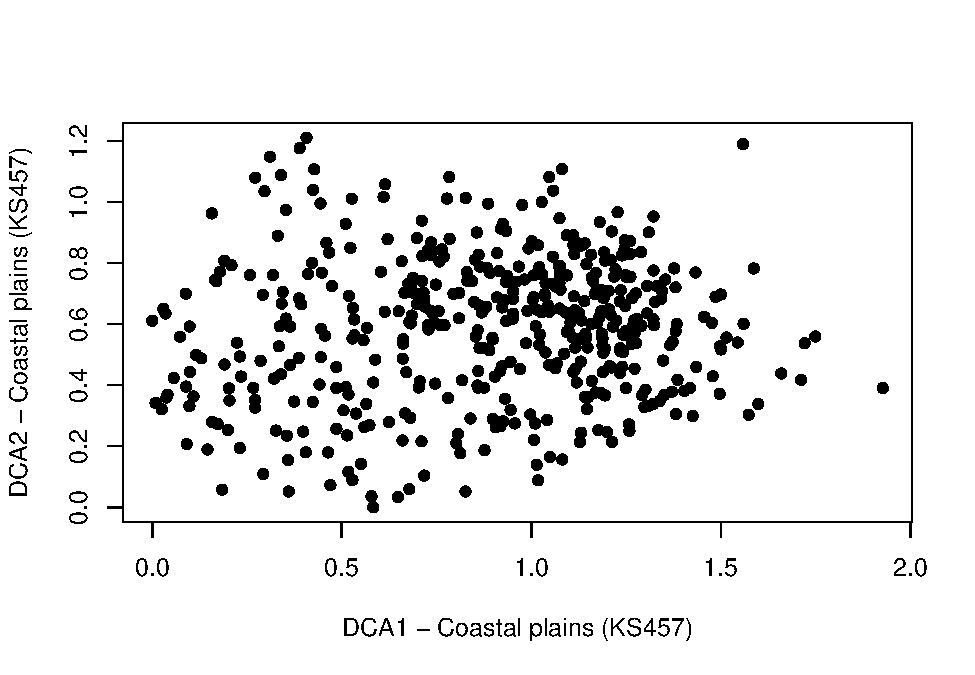
\includegraphics{Landscape_analysis_example_4_files/figure-latex/unnamed-chunk-3-1.pdf}

There were no visible artifacts in the ordination charts. The
correlation analysis, the vector charts and the iso-line charts show a
strong first axis related to land use (infrastructure and agricultural
character) that appears to be conditioned by an underlying
geo-ecological gradient from inner to outer coast. Second axis is
strongly related to relief.

\begin{table}[H]
\centering
\begin{tabular}{l|l|r|r|r|r}
\hline
Variable & Description & GNMDS1 & GNMDS2 & GNMDS3 & GNMDS4\\
\hline
Gab\_nae & No commercial buildings & 0.6345 & -0.1164 & -0.0294 & -0.0092\\
\hline
Gab\_fi & No fisheries-related buildings & 0.3166 & -0.0682 & 0.1576 & -0.0607\\
\hline
Gab\_a & PA built-up & 0.7328 & -0.0514 & -0.0632 & -0.0397\\
\hline
Flat\_a & PA flat terrain & -0.0920 & -0.5626 & 0.2041 & 0.1333\\
\hline
Vmag\_a & PA regulated magazine & 0.0638 & 0.0458 & -0.0305 & 0.0313\\
\hline
Vei\_b\_a & PA road & 0.6270 & -0.0403 & 0.0441 & 0.0764\\
\hline
Ktkmo\_a & PA thick layer of till & 0.2496 & 0.0351 & 0.0825 & 0.2250\\
\hline
Tpi1l\_a & PA depressions & 0.1171 & 0.5584 & -0.0046 & -0.0476\\
\hline
Tpi1h\_a & PA convex terrain & 0.0115 & 0.4749 & -0.2350 & -0.2408\\
\hline
Tpi1\_mp & Terrain form TPI1, numerical, mean & -0.0787 & 0.0753 & -0.1994 & -0.1974\\
\hline
Stroms\_a & PA strong ocean current & 0.0130 & -0.0281 & 0.1729 & 0.1029\\
\hline
Stromn\_a & PA normal ocean current & -0.5201 & -0.1313 & 0.1621 & -0.0064\\
\hline
Stroml\_a & PA weak ocean current & 0.1040 & 0.1434 & -0.2647 & 0.0612\\
\hline
River\_a & PA large river & 0.1955 & -0.1176 & 0.1526 & 0.1342\\
\hline
Sti\_a & PA trail, path & 0.1018 & -0.0506 & -0.0624 & 0.0061\\
\hline
Steep\_a & PA steep terrain/slope & 0.0664 & 0.6571 & -0.0831 & -0.0625\\
\hline
Kskred\_a & PA landslide soil & -0.0134 & 0.2100 & 0.3115 & 0.1613\\
\hline
Setr\_s & No summer mountain pasture & 0.1523 & 0.0005 & 0.0472 & -0.0194\\
\hline
Sefr\_a & PA old buildings & 0.5703 & -0.0920 & -0.0622 & -0.1033\\
\hline
Rug3\_m & Terrain ruggedness VRM3, mean & 0.0404 & 0.6617 & -0.0259 & -0.1666\\
\hline
Rr1\_m & Altitudinal range & 0.0752 & 0.7185 & -0.0293 & 0.0011\\
\hline
Brich\_a & PA lime-rich bedrock & 0.0159 & 0.0992 & -0.1475 & 0.1324\\
\hline
Bpoor\_a & PA lime-poor bedrock geology & 0.0641 & -0.0189 & 0.0535 & -0.2003\\
\hline
Rd\_anl\_a & PA reindeer husbandry facilities & 0.0533 & 0.1007 & 0.0276 & 0.1174\\
\hline
Bplu\_a & PA plutonic rock & 0.0541 & -0.1586 & 0.0252 & -0.3956\\
\hline
Bvul\_a & PA volcanic rock & 0.1879 & -0.0016 & -0.0087 & -0.1046\\
\hline
Bavstn\_a & PA sedimentary rock & 0.1844 & -0.1174 & -0.1346 & 0.1115\\
\hline
Bomd\_a & PA metamorphic rock & -0.0386 & 0.1951 & 0.0493 & 0.1713\\
\hline
Land\_a & PA terrestrial area & 0.6629 & 0.0369 & 0.0937 & -0.1296\\
\hline
Build\_a & PA built-up area & 0.4657 & -0.1377 & -0.0752 & -0.0331\\
\hline
City\_a & PA town/city area & 0.1699 & -0.0631 & -0.1038 & 0.0314\\
\hline
Mire\_a & PA mire & 0.3114 & 0.0618 & 0.3063 & -0.1761\\
\hline
Meant\_a & PA moderate slope & 0.1062 & 0.3618 & -0.2532 & -0.1399\\
\hline
Maro\_s & No marine islands & -0.1609 & -0.1324 & 0.0874 & -0.4627\\
\hline
Kmar\_a & PA marine deposits & 0.3888 & -0.1691 & 0.0652 & 0.3365\\
\hline
Lled\_a & PA power lines & 0.6407 & -0.0074 & 0.0375 & -0.0425\\
\hline
Klac\_a & PA lacustrine deposits & 0.0278 & -0.0492 & 0.0674 & 0.0588\\
\hline
Kelv\_a & PA glaciofluvial deposits & 0.2298 & 0.0004 & 0.0094 & 0.1849\\
\hline
Kbf\_a & PA exposed bedrock & -0.5130 & 0.1119 & -0.1193 & -0.1483\\
\hline
Lake\_a & PA freshwater lake & 0.2853 & 0.0324 & 0.2846 & -0.2841\\
\hline
Innoy\_s & No freshwater lake islands & 0.2519 & 0.0402 & 0.1403 & -0.2380\\
\hline
Er\_m & Hydrographic index, ER, mean & -0.1692 & -0.0660 & -0.1416 & -0.2859\\
\hline
R\_net\_a & PA river & 0.5439 & 0.1233 & 0.1754 & 0.0161\\
\hline
Ekspve\_a & PA exposed coast & -0.4350 & -0.0564 & 0.2315 & 0.1983\\
\hline
Ekspmo\_a & PA sligyhtly exposed coast & -0.3992 & -0.1357 & 0.1847 & -0.0639\\
\hline
Ekspbe\_a & PA slightly protected coast & 0.0284 & 0.0154 & -0.2599 & -0.0083\\
\hline
Inns\_s & No lakes & 0.1119 & -0.0461 & 0.4004 & -0.3517\\
\hline
Cul\_u\_s & No cultural heritage sites outdoors & 0.2744 & -0.1048 & -0.1217 & 0.0378\\
\hline
Cul\_t\_s & No technical heritage sites & 0.2435 & 0.0028 & -0.0328 & 0.0082\\
\hline
Cul\_m\_s & No marine cultural heritage sites & 0.2090 & 0.0296 & -0.1025 & -0.1863\\
\hline
Cul\_k\_s & No church ruins & 0.3534 & -0.1442 & -0.0394 & -0.0059\\
\hline
Cul\_b\_s & No ancient rock art sites & 0.2314 & -0.0738 & -0.0586 & 0.0975\\
\hline
Cul\_a\_s & No archeological heritage sites & 0.5134 & -0.0412 & 0.0209 & 0.0436\\
\hline
Cre\_b\_a & PA steep coast & 0.0351 & 0.5233 & 0.2241 & 0.0719\\
\hline
Cre\_f\_a & PA flat coast & -0.0716 & -0.5412 & 0.1673 & -0.0322\\
\hline
Crug3\_m & Coastal ruggedness, VRM3, mean & -0.0147 & 0.6764 & -0.0566 & -0.0172\\
\hline
Crug9\_m & Coastal ruggedness, coarse scale, VRM9, mean & 0.0205 & 0.7286 & 0.0134 & 0.0165\\
\hline
Cr3\_u\_a & PA rugged coast & 0.0120 & 0.5767 & 0.0929 & -0.0299\\
\hline
Cr3\_r\_a & PA smooth/flat coast & 0.1328 & -0.1676 & 0.1194 & -0.3568\\
\hline
Ccom\_m & Coastal complexity & 0.1233 & 0.0012 & 0.1075 & -0.4223\\
\hline
C\_kk\_a & PA complex coastline & 0.0370 & -0.1276 & 0.1500 & -0.5028\\
\hline
C\_ek\_a & PA simple coastline Gab\_fi & 0.0708 & 0.1907 & -0.0039 & 0.3369\\
\hline
Bohei\_a & PA boreal heaths & 0.2844 & 0.0965 & 0.4234 & -0.0554\\
\hline
Asp\_s\_a & PA south facing terrain & -0.0277 & -0.0953 & -0.0417 & -0.1100\\
\hline
Asp\_n\_a & PA north facing terrain & -0.1435 & 0.0227 & 0.0876 & 0.0632\\
\hline
Abygg\_a & PA large buildings & 0.4676 & -0.1406 & -0.0750 & -0.0371\\
\hline
Araaf\_a & PA open areas & 0.2580 & -0.0311 & 0.3528 & -0.1493\\
\hline
Arbar\_a & PA coniferous forest & 0.5742 & 0.0267 & -0.1798 & -0.1160\\
\hline
Arbla\_a & PA mixed boreal forest & 0.5456 & 0.0191 & -0.2502 & -0.0497\\
\hline
Arfull\_a & PA arable land & 0.5974 & -0.1116 & -0.0122 & 0.1307\\
\hline
Arlov\_a & PA deciduous forest & 0.5743 & 0.0956 & -0.0356 & -0.0475\\
\hline
Arover\_a & PA surface cultivated land & 0.3461 & 0.0327 & 0.2269 & -0.0626\\
\hline
Dismire & Distance to mire, mean & -0.3504 & -0.1510 & -0.2023 & 0.1649\\
\hline
Dislake & Distance to lake, mean & -0.3049 & -0.1074 & -0.2768 & 0.2448\\
\hline
Discoast & Distance to coast, mean & -0.3573 & -0.0455 & 0.2784 & -0.2392\\
\hline
Guro\_t\_a & PA rugged terrain & 0.0282 & 0.5437 & 0.2286 & -0.0350\\
\hline
Tpi6l\_a & PA rugged terrain, TPI6 & 0.1665 & 0.1377 & 0.0645 & 0.1714\\
\hline
Sn\_imp & PA impediment & -0.1980 & 0.1446 & 0.2950 & 0.1299\\
\hline
Sn\_flekk & PA patchy open treeless area & -0.1862 & 0.1571 & 0.4446 & -0.0965\\
\hline
Sn\_lav & PA lichen heath & 0.1057 & -0.0434 & -0.0359 & 0.0867\\
\hline
Sn\_torr & PA dry heath/open areas & -0.0046 & 0.0888 & 0.4795 & -0.2194\\
\hline
Sn\_frisk & PA moist/fresh heath/open areas & 0.0485 & 0.0720 & 0.4784 & -0.0170\\
\hline
Sn\_ureg & PA unregistered heath/open areas & 0.3218 & -0.2076 & -0.0564 & 0.1267\\
\hline
Oyst\_i & Inverse island size & -0.5057 & -0.0913 & -0.1215 & -0.1944\\
\hline
\end{tabular}
\end{table}

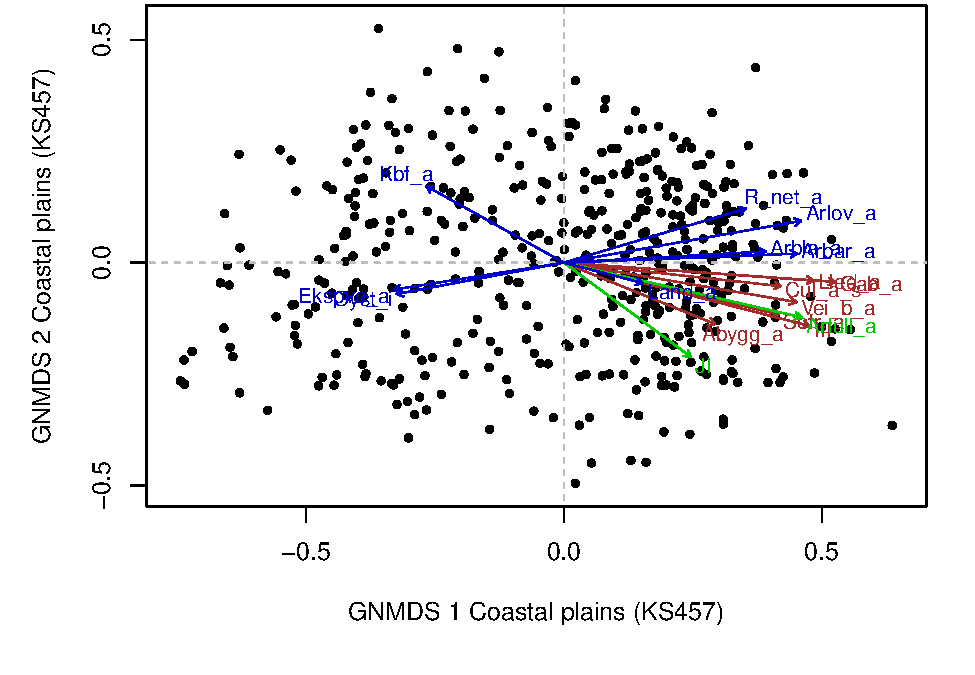
\includegraphics{Landscape_analysis_example_4_files/figure-latex/unnamed-chunk-9-1.pdf}

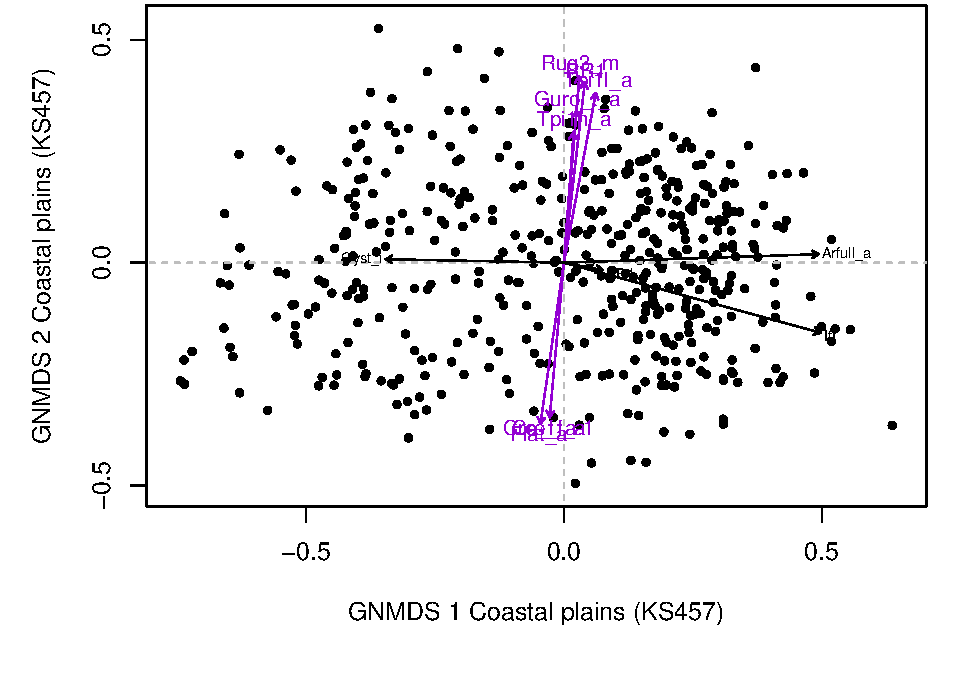
\includegraphics{Landscape_analysis_example_4_files/figure-latex/unnamed-chunk-10-1.pdf}

\hypertarget{complementary-observations-axis-1-and-2}{%
\paragraph{Complementary observations, axis 1 and
2:}\label{complementary-observations-axis-1-and-2}}

\begin{itemize}
\tightlist
\item
  One OU belongs to OI Class 6 (big city). This is Id 2916 Oslo city,
  which occupies the extreme position along GNMDS axis 1.
\item
  Agricultural intensity is associated with positive scores for GNMDS 1,
  and a certain degree of infrastructure (similar to IfI ≈ 4) is a
  prerequisite for amount/degree of agricultural land use intensity. The
  relationship between JI and IfI is slightly unimodal, that is, the
  agricultural land use intensity is strongest when the amount/degree of
  infrastructure is relatively high, but decreases again when the
  amount/degree of infrastructure is very high.
\item
  The proportion of the area with deciduous forest (Arlov\_a) is 0 at
  the outer parts of the archipelago (SN = 5; there are 156 OUs with
  Arlov = 0), but increases inward towards larger islands and on the
  mainland.
\item
  The figure at the bottom left shows a clear (inverse) island size
  gradient, with a considerable variation in landscape characteristics
  related to the archipelago properties, first and foremost when the
  islands are smaller than 100 km2 (Oyst\_i \textgreater{} 0.643). This
  opens the possibility that the complex gradient expressed on axis 1 is
  actually composed of two CLGs.
\item
  Among the 69 OUs in KS lacking infrastructure (IfI = 0), all of the 56
  as a largest island smaller than 1 km. Islands with significant
  infrastructure are generally much larger; one exception is Id 4038
  which has Oyst\_i = 0.8647 and IfI = 9.34. This polygon is located on
  the west and south part of Nøtterøy.
\item
  It is noteworthy that the topographic variables give such a strong
  signal when there is so little topography variation within costal
  plains.
\end{itemize}

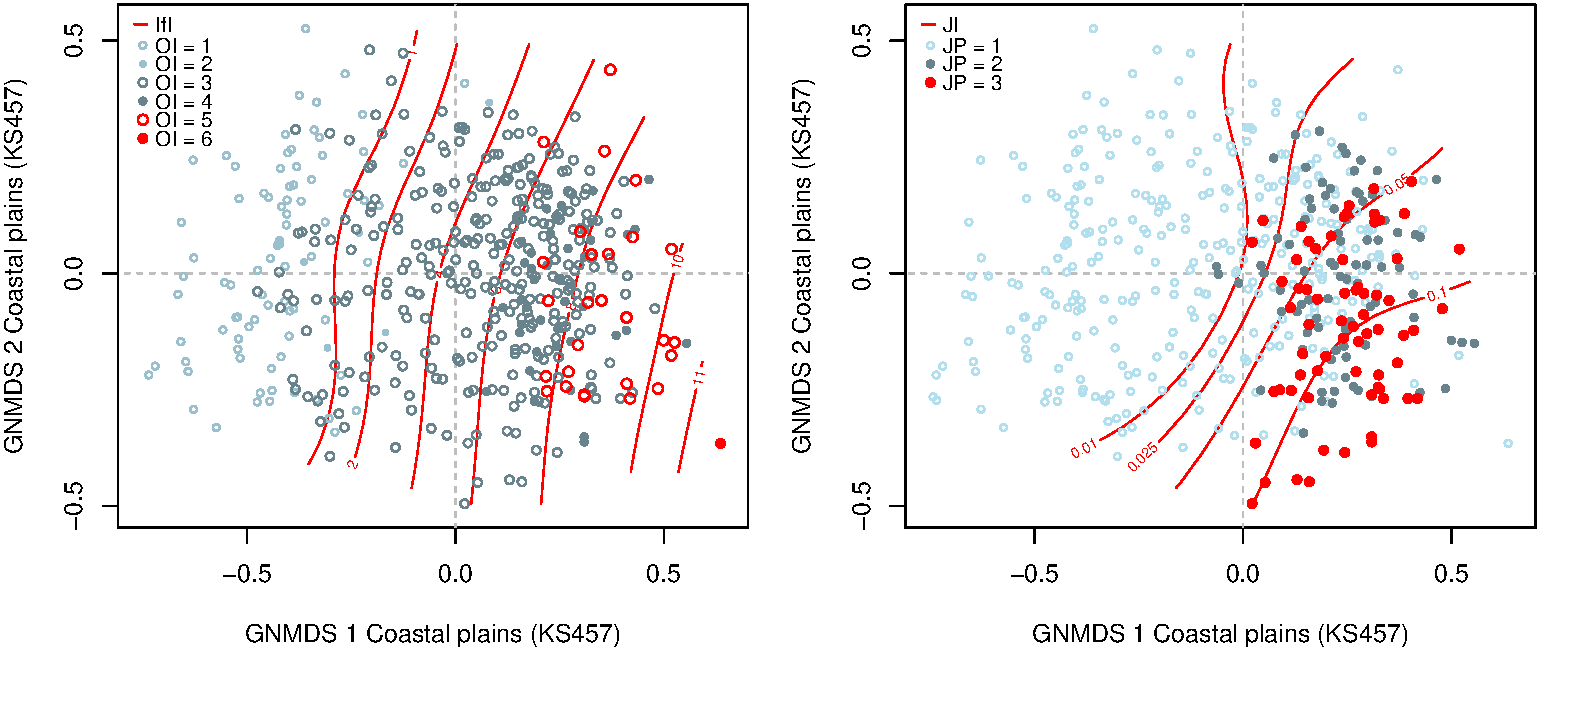
\includegraphics{Landscape_analysis_example_4_files/figure-latex/unnamed-chunk-11-1.pdf}

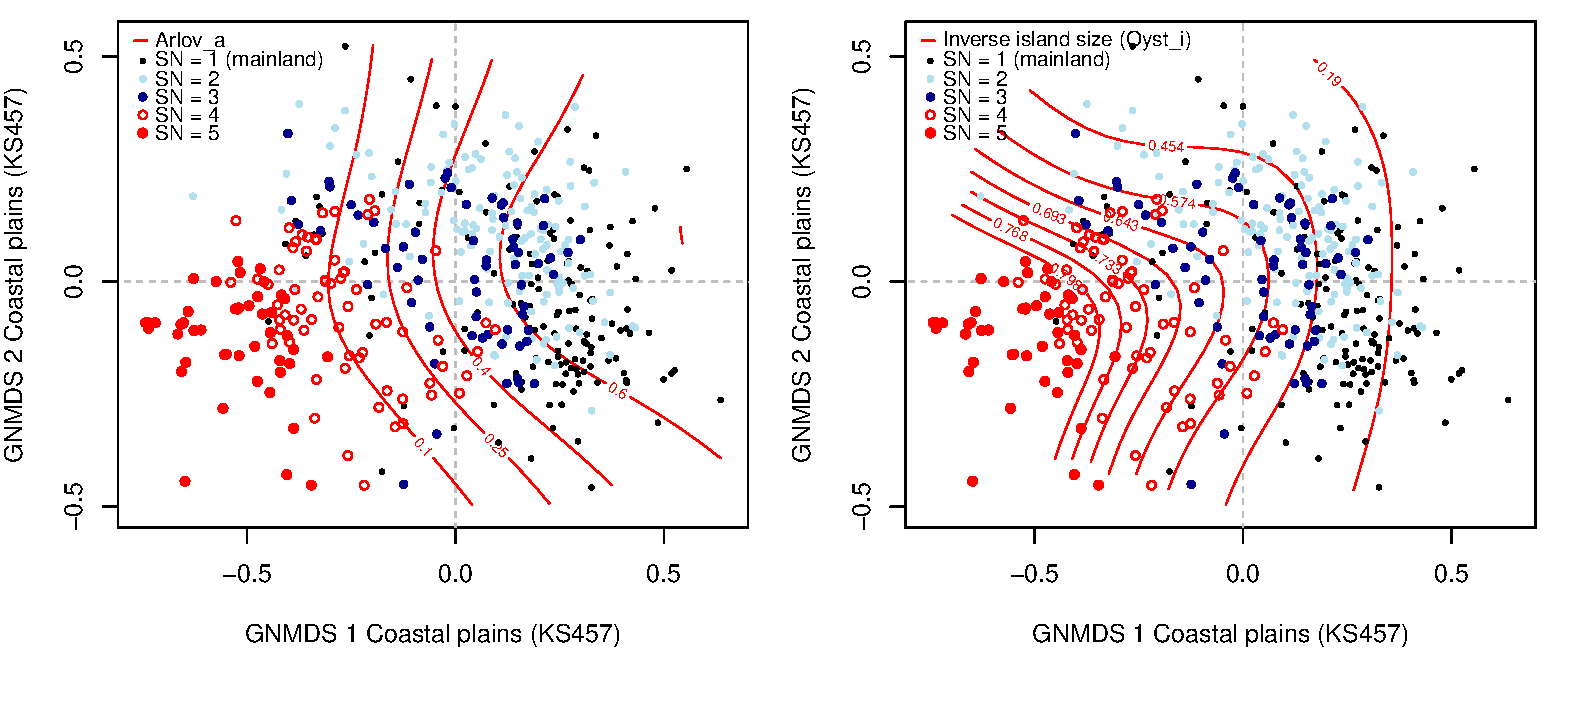
\includegraphics{Landscape_analysis_example_4_files/figure-latex/unnamed-chunk-12-1.pdf}

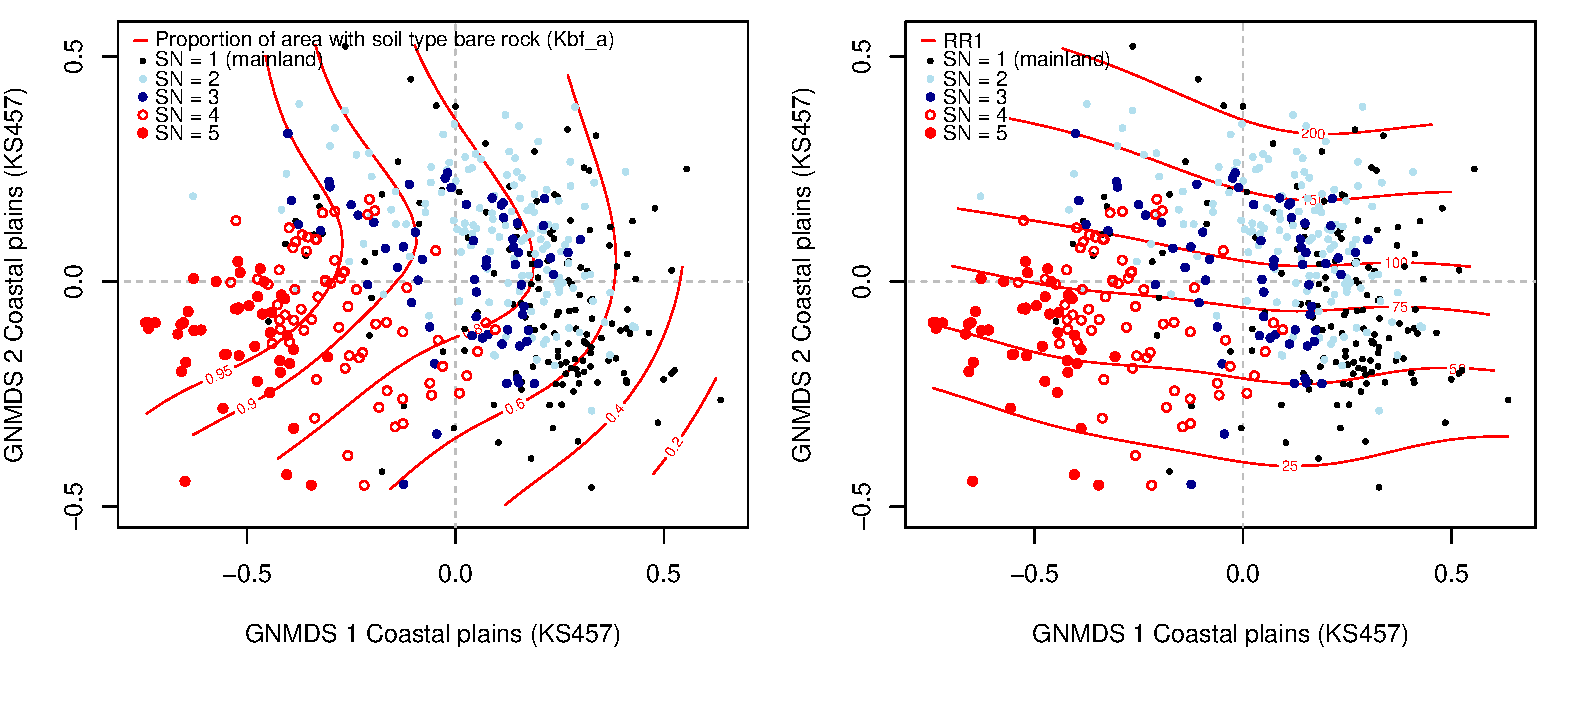
\includegraphics{Landscape_analysis_example_4_files/figure-latex/unnamed-chunk-13-1.pdf}

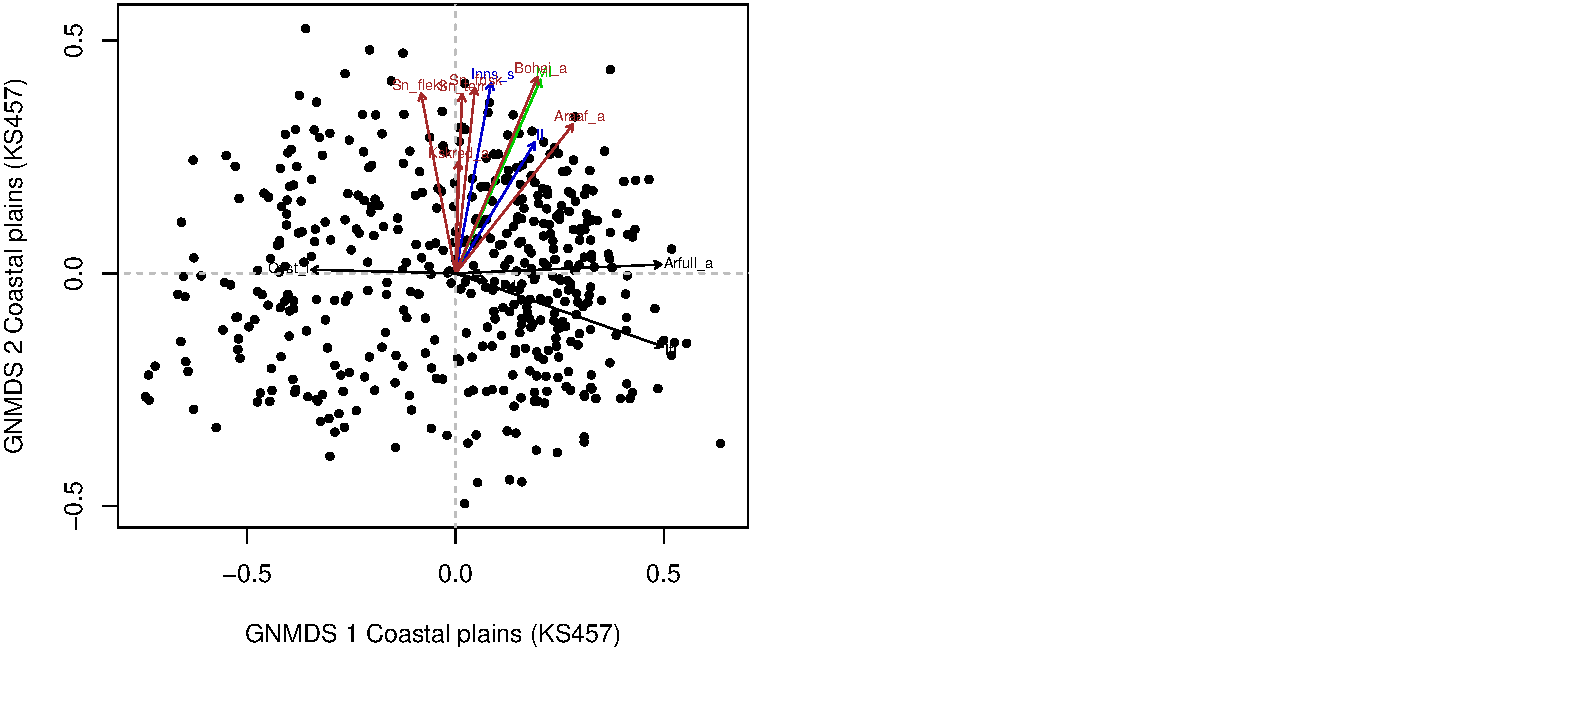
\includegraphics{Landscape_analysis_example_4_files/figure-latex/unnamed-chunk-14-1.pdf}

Investigated whether there could be grounds for dividing KS into two
major types based on dominant soil, parallel to the classification of
inland irregular plains by looking at the variation in occurrence of
selected soil classes JK1 (based on 50\% proportion of area) and JK2
(based of 25\% proportion of area) in the ordination chart. For JK1 the
distribution is: B (\textgreater{} 50\% bare rock): 346; H
(\textgreater{} 50\% marine deposits): 27; 0 (none) 61. For JK2
(\textgreater{} 25\% proportion of area), 83 OUs belong to H. The
distribution of the earth classes in the GNMDS diagram with axis 1 and 2
shows that there is a relationship between earth and axis 1, but that it
is not very strong (there are scattered OUs with bare rock scattered all
the way between OUs with larger or less amount of marine deposits).

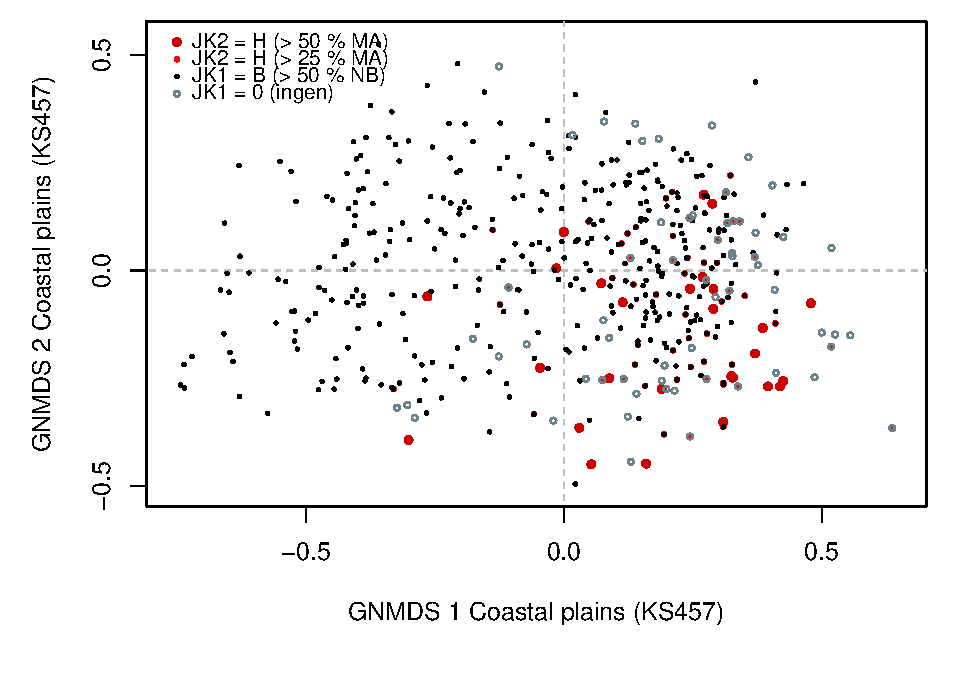
\includegraphics{Landscape_analysis_example_4_files/figure-latex/unnamed-chunk-15-1.pdf}

Conclusion:

There is no basis for dividing coastal plains into two major types on
the basis of dominant soil.

Parallel RDA analyzes with factor variables one and the continuous
analysis variables as alternative ways of representing soil variation
showed that both single analysis variables Kmar\_a and Kbf\_a explained
more variation in the data set KS457 (0.06004 and 0.05969) than factor
variables JK1 and JK2 (0.0387, respectively). Therefore, used the
analysis variables to characterize soil as a CLG candidate. The
ordination analysis and interpretation identified the following hCLG
candidates by the three functional variables categories G, U and A
(thematically slightly marginal variables are highlighted in gray; the
absolute value of the correlation coefficient with the relevant GNMDS
axis in parentheses):

(G1) Relieff (RE; Axis 2): Crug9\_m (0.7286) RR1 (0.7185), Crug3\_m
(0.6764), Rug3\_m (0.6617), Steep\_a (0.6572), Cr3\_u\_a (0.5767),
Flat\_a (0.5626), Tpi1l\_a (0.5585), Guro\_t\_a (0.5437), Cre\_f\_a
(0.5412), Cre\_b\_a (0.5234), Tpi1h\_a (0.4750) (G2) Indre-outer coast
(IYK; Axis 1/2): Land\_a (0.5702), Stromn\_a (0.5203), Oyst\_i (0.5057),
R\_net\_a (0.5440), Ekspve\_a (0.4351) (G3) Vannpreg (VP; Axis 1/3/4:
Inns\_s (0.4005), Dismire (0.3505), MI (0.3310), II (0.3051), Dislake
(0.3049)

\hypertarget{tallfesting-av-klg-kandidatenes-relative-viktighet-ved-variasjonsoppdelingsanalyse}{%
\paragraph{Tallfesting av KLG-kandidatenes relative viktighet ved
variasjonsoppdelingsanalyse}\label{tallfesting-av-klg-kandidatenes-relative-viktighet-ved-variasjonsoppdelingsanalyse}}

\begin{Shaded}
\begin{Highlighting}[]
\CommentTok{#Datasett: av}

\CommentTok{#Bestemmer total variasjon}

\NormalTok{vo0 <-}\StringTok{ }\KeywordTok{rda}\NormalTok{(av}\OperatorTok{~+}\DecValTok{1}\NormalTok{,}\DataTypeTok{scale=}\NormalTok{T)  }\CommentTok{#scale = T gjør at dataene blir sentrert og standardisert ved deling med SD}
\NormalTok{vo0}
\end{Highlighting}
\end{Shaded}

\begin{verbatim}
## Call: rda(formula = av ~ +1, scale = T)
## 
##               Inertia Rank
## Total              84     
## Unconstrained      84   84
## Inertia is correlations 
## 
## Eigenvalues for unconstrained axes:
##    PC1    PC2    PC3    PC4    PC5    PC6    PC7    PC8 
## 13.689  9.256  6.466  5.348  3.291  3.036  2.548  2.308 
## (Showing 8 of 84 unconstrained eigenvalues)
\end{verbatim}

\begin{Shaded}
\begin{Highlighting}[]
\NormalTok{voG1a <-}\StringTok{ }\KeywordTok{rda}\NormalTok{(av}\OperatorTok{~}\NormalTok{RR1,}\DataTypeTok{scale=}\NormalTok{T)}
\NormalTok{voG1a}
\end{Highlighting}
\end{Shaded}

\begin{verbatim}
## Call: rda(formula = av ~ RR1, scale = T)
## 
##                Inertia Proportion Rank
## Total         84.00000    1.00000     
## Constrained    7.36127    0.08763    1
## Unconstrained 76.63873    0.91237   84
## Inertia is correlations 
## 
## Eigenvalues for constrained axes:
##  RDA1 
## 7.361 
## 
## Eigenvalues for unconstrained axes:
##    PC1    PC2    PC3    PC4    PC5    PC6    PC7    PC8 
## 13.526  6.519  5.408  3.466  3.184  2.781  2.380  2.179 
## (Showing 8 of 84 unconstrained eigenvalues)
\end{verbatim}

\begin{Shaded}
\begin{Highlighting}[]
\NormalTok{tvoG1a <-}\StringTok{ }\KeywordTok{permutest}\NormalTok{(voG1a,}\DataTypeTok{permutations=}\DecValTok{9999}\NormalTok{)}
\NormalTok{tvoG1a}
\end{Highlighting}
\end{Shaded}

\begin{verbatim}
## 
## Permutation test for rda under reduced model 
## 
## Permutation: free
## Number of permutations: 9999
##  
## Model: rda(formula = av ~ RR1, scale = T)
## Permutation test for all constrained eigenvalues
##           Df Inertia      F Pr(>F)    
## Model      1   7.361 43.703  1e-04 ***
## Residual 455  76.639                  
## ---
## Signif. codes:  0 '***' 0.001 '**' 0.01 '*' 0.05 '.' 0.1 ' ' 1
\end{verbatim}

\begin{Shaded}
\begin{Highlighting}[]
\NormalTok{voG1b <-}\StringTok{ }\KeywordTok{rda}\NormalTok{(av}\OperatorTok{~}\NormalTok{Crug9_m,}\DataTypeTok{scale=}\NormalTok{T)}
\NormalTok{voG1b}
\end{Highlighting}
\end{Shaded}

\begin{verbatim}
## Call: rda(formula = av ~ Crug9_m, scale = T)
## 
##                Inertia Proportion Rank
## Total         84.00000    1.00000     
## Constrained    7.70551    0.09173    1
## Unconstrained 76.29449    0.90827   83
## Inertia is correlations 
## 
## Eigenvalues for constrained axes:
##  RDA1 
## 7.706 
## 
## Eigenvalues for unconstrained axes:
##    PC1    PC2    PC3    PC4    PC5    PC6    PC7    PC8 
## 13.596  6.538  5.436  3.501  3.058  2.548  2.394  2.142 
## (Showing 8 of 83 unconstrained eigenvalues)
\end{verbatim}

\begin{Shaded}
\begin{Highlighting}[]
\NormalTok{tvoG1b <-}\StringTok{ }\KeywordTok{permutest}\NormalTok{(voG1b,}\DataTypeTok{permutations=}\DecValTok{9999}\NormalTok{)}
\NormalTok{tvoG1b}
\end{Highlighting}
\end{Shaded}

\begin{verbatim}
## 
## Permutation test for rda under reduced model 
## 
## Permutation: free
## Number of permutations: 9999
##  
## Model: rda(formula = av ~ Crug9_m, scale = T)
## Permutation test for all constrained eigenvalues
##           Df Inertia      F Pr(>F)    
## Model      1   7.706 45.954  1e-04 ***
## Residual 455  76.294                  
## ---
## Signif. codes:  0 '***' 0.001 '**' 0.01 '*' 0.05 '.' 0.1 ' ' 1
\end{verbatim}

voG1c \textless{}- rda(av\textasciitilde{}Rug3\_m,scale=T) voG1c tvoG1c
\textless{}- permutest(voG1c,permutations=9999) tvoG1c voG1d
\textless{}- rda(av\textasciitilde{}Cr3\_u\_a,scale=T) voG1d tvoG1d
\textless{}- permutest(voG1d,permutations=9999) tvoG1d voG1e
\textless{}- rda(av\textasciitilde{}Flat\_a,scale=T) voG1e tvoG1e
\textless{}- permutest(voG1e,permutations=9999) tvoG1e voG1f
\textless{}- rda(av\textasciitilde{}Tpi1l\_a,scale=T) voG1f tvoG1f
\textless{}- permutest(voG1f,permutations=9999) tvoG1f voG1g
\textless{}- rda(av\textasciitilde{}Guro\_t\_a,scale=T) voG1g tvoG1g
\textless{}- permutest(voG1g,permutations=9999) tvoG1g voG1h
\textless{}- rda(av\textasciitilde{}Cre\_f\_a,scale=T) voG1h tvoG1h
\textless{}- permutest(voG1h,permutations=9999) tvoG1h voG1i
\textless{}- rda(av\textasciitilde{}Cre\_b\_a,scale=T) voG1i tvoG1i
\textless{}- permutest(voG1i,permutations=9999) tvoG1i voG1j
\textless{}- rda(av\textasciitilde{}Tpi1h\_a,scale=T) voG1j tvoG1j
\textless{}- permutest(voG1j,permutations=9999) tvoG1j voG1k
\textless{}- rda(av\textasciitilde{}Steep\_a,scale=T) voG1k tvoG1k
\textless{}- permutest(voG1k,permutations=9999) tvoG1k voG1l
\textless{}- rda(av\textasciitilde{}Crug3\_m,scale=T) voG1l tvoG1l
\textless{}- permutest(voG1l,permutations=9999) tvoG1l

\begin{Shaded}
\begin{Highlighting}[]
\NormalTok{voG1ca <-}\StringTok{ }\KeywordTok{rda}\NormalTok{(av}\OperatorTok{~}\NormalTok{RR1}\OperatorTok{+}\KeywordTok{Condition}\NormalTok{(Rug3_m),}\DataTypeTok{scale=}\NormalTok{T)}
\NormalTok{voG1ca}
\end{Highlighting}
\end{Shaded}

\begin{verbatim}
## Call: rda(formula = av ~ RR1 + Condition(Rug3_m), scale = T)
## 
##                Inertia Proportion Rank
## Total         84.00000    1.00000     
## Conditional    8.40616    0.10007    1
## Constrained    1.82984    0.02178    1
## Unconstrained 73.76400    0.87814   83
## Inertia is correlations 
## 
## Eigenvalues for constrained axes:
##   RDA1 
## 1.8298 
## 
## Eigenvalues for unconstrained axes:
##    PC1    PC2    PC3    PC4    PC5    PC6    PC7    PC8 
## 13.518  6.346  4.960  3.184  2.908  2.496  2.220  2.085 
## (Showing 8 of 83 unconstrained eigenvalues)
\end{verbatim}

\begin{Shaded}
\begin{Highlighting}[]
\NormalTok{tvoG1ca <-}\StringTok{ }\KeywordTok{permutest}\NormalTok{(voG1ca,}\DataTypeTok{permutations=}\DecValTok{9999}\NormalTok{)}
\NormalTok{tvoG1ca}
\end{Highlighting}
\end{Shaded}

\begin{verbatim}
## 
## Permutation test for rda under reduced model 
## 
## Permutation: free
## Number of permutations: 9999
##  
## Model: rda(formula = av ~ RR1 + Condition(Rug3_m), scale = T)
## Permutation test for all constrained eigenvalues
##           Df Inertia      F Pr(>F)    
## Model      1   1.830 11.262  1e-04 ***
## Residual 454  73.764                  
## ---
## Signif. codes:  0 '***' 0.001 '**' 0.01 '*' 0.05 '.' 0.1 ' ' 1
\end{verbatim}

voG1cb \textless{}-
rda(av\textasciitilde{}Crug9\_m+Condition(Rug3\_m),scale=T) voG1cb
tvoG1cb \textless{}- permutest(voG1cb,permutations=9999) tvoG1cb

\begin{Shaded}
\begin{Highlighting}[]
\NormalTok{voG1cd <-}\StringTok{ }\KeywordTok{rda}\NormalTok{(av}\OperatorTok{~}\NormalTok{Cr3_u_a}\OperatorTok{+}\KeywordTok{Condition}\NormalTok{(Rug3_m),}\DataTypeTok{scale=}\NormalTok{T)}
\NormalTok{voG1cd}
\end{Highlighting}
\end{Shaded}

\begin{verbatim}
## Call: rda(formula = av ~ Cr3_u_a + Condition(Rug3_m), scale = T)
## 
##                Inertia Proportion Rank
## Total         84.00000    1.00000     
## Conditional    8.40616    0.10007    1
## Constrained    1.35837    0.01617    1
## Unconstrained 74.23547    0.88376   82
## Inertia is correlations 
## 
## Eigenvalues for constrained axes:
##   RDA1 
## 1.3584 
## 
## Eigenvalues for unconstrained axes:
##    PC1    PC2    PC3    PC4    PC5    PC6    PC7    PC8 
## 13.519  6.464  4.968  3.494  3.035  2.552  2.218  2.094 
## (Showing 8 of 82 unconstrained eigenvalues)
\end{verbatim}

\begin{Shaded}
\begin{Highlighting}[]
\NormalTok{tvoG1cd <-}\StringTok{ }\KeywordTok{permutest}\NormalTok{(voG1cd,}\DataTypeTok{permutations=}\DecValTok{9999}\NormalTok{)}
\NormalTok{tvoG1cd}
\end{Highlighting}
\end{Shaded}

\begin{verbatim}
## 
## Permutation test for rda under reduced model 
## 
## Permutation: free
## Number of permutations: 9999
##  
## Model: rda(formula = av ~ Cr3_u_a + Condition(Rug3_m), scale = T)
## Permutation test for all constrained eigenvalues
##           Df Inertia      F Pr(>F)    
## Model      1   1.358 8.3073  1e-04 ***
## Residual 454  74.235                  
## ---
## Signif. codes:  0 '***' 0.001 '**' 0.01 '*' 0.05 '.' 0.1 ' ' 1
\end{verbatim}

voG1ce \textless{}-
rda(av\textasciitilde{}Flat\_a+Condition(Rug3\_m),scale=T) voG1ce
tvoG1ce \textless{}- permutest(voG1ce,permutations=9999) tvoG1ce voG1cf
\textless{}- rda(av\textasciitilde{}Tpi1l\_a+Condition(Rug3\_m),scale=T)
voG1cf tvoG1cf \textless{}- permutest(voG1cf,permutations=9999) tvoG1cf
voG1cg \textless{}-
rda(av\textasciitilde{}Guro\_t\_a+Condition(Rug3\_m),scale=T) voG1cg
tvoG1cg \textless{}- permutest(voG1cg,permutations=9999) tvoG1cg voG1ch
\textless{}-
rda(av\textasciitilde{}Cre\_f\_a+Condition(Rug3\_m),scale=T) voG1ch
tvoG1ch \textless{}- permutest(voG1ch,permutations=9999) tvoG1ch voG1ci
\textless{}-
rda(av\textasciitilde{}Cre\_b\_a+Condition(Rug3\_m),scale=T) voG1ci
tvoG1ci \textless{}- permutest(voG1ci,permutations=9999) tvoG1ci voG1cj
\textless{}- rda(av\textasciitilde{}Tpi1h\_a+Condition(Rug3\_m),scale=T)
voG1cj tvoG1cj \textless{}- permutest(voG1cj,permutatioks=9999) tvoG1cj
voG1ck \textless{}-
rda(av\textasciitilde{}Steep\_a+Condition(Rug3\_m),scale=T) voG1ck
tvoG1ck \textless{}- permutest(voG1ck,permutations=9999) tvoG1ck voG1cl
\textless{}- rda(av\textasciitilde{}Crug3\_m+Condition(Rug3\_m),scale=T)
voG1cl tvoG1cl \textless{}- permutest(voG1cl,permutations=9999) tvoG1cl

voG1cja \textless{}-
rda(av\textasciitilde{}RR1+Condition(Rug3\_m+Tpi1h\_a),scale=T) voG1cja
tvoG1cja \textless{}- permutest(voG1cja,permutations=9999) tvoG1cja

voG1cjb \textless{}-
rda(av\textasciitilde{}Crug9\_m+Condition(Rug3\_m+Tpi1h\_a),scale=T)
voG1cjb tvoG1cjb \textless{}- permutest(voG1cjb,permutations=9999)
tvoG1cjb voG1cjd \textless{}-
rda(av\textasciitilde{}Cr3\_u\_a+Condition(Rug3\_m+Tpi1h\_a),scale=T)
voG1cjd tvoG1cjd \textless{}- permutest(voG1cjd,permutations=9999)
tvoG1cjd voG1cje \textless{}-
rda(av\textasciitilde{}Flat\_a+Condition(Rug3\_m+Tpi1h\_a),scale=T)
voG1cje tvoG1cje \textless{}- permutest(voG1cje,permutations=9999)
tvoG1cje voG1cjf \textless{}-
rda(av\textasciitilde{}Tpi1l\_a+Condition(Rug3\_m+Tpi1h\_a),scale=T)
voG1cjf tvoG1cjf \textless{}- permutest(voG1cjf,permutations=9999)
tvoG1cjf voG1cjg \textless{}-
rda(av\textasciitilde{}Guro\_t\_a+Condition(Rug3\_m+Tpi1h\_a),scale=T)
voG1cjg tvoG1cjg \textless{}- permutest(voG1cjg,permutations=9999)
tvoG1cjg voG1cjh \textless{}-
rda(av\textasciitilde{}Cre\_f\_a+Condition(Rug3\_m+Tpi1h\_a),scale=T)
voG1cjh tvoG1cjh \textless{}- permutest(voG1cjh,permutations=9999)
tvoG1cjh voG1cji \textless{}-
rda(av\textasciitilde{}Cre\_b\_a+Condition(Rug3\_m+Tpi1h\_a),scale=T)
voG1cji tvoG1cji \textless{}- permutest(voG1cji,permutations=9999)
tvoG1cji voG1cjl \textless{}-
rda(av\textasciitilde{}Crug3\_m+Condition(Rug3\_m+Tpi1h\_a),scale=T)
voG1cjl tvoG1cjl \textless{}- permutest(voG1cjl,permutations=9999)
tvoG1cjl

voG1cjhf \textless{}-
rda(av\textasciitilde{}Tpi1l\_a+Condition(Rug3\_m+Tpi1h\_a+Cre\_f\_a),scale=T)
voG1cjhf tvoG1cjhf \textless{}- permutest(voG1cjhf,permutations=9999)
tvoG1cjhf voG1cjhk \textless{}-
rda(av\textasciitilde{}Crug3\_m+Condition(Rug3\_m+Tpi1h\_a+Cre\_f\_a),scale=T)
voG1cjhk tvoG1cjhk \textless{}- permutest(voG1cjhk,permutations=99)
tvoG1cjhk

voG2a \textless{}- rda(av\textasciitilde{}Oyst\_i,scale=T) voG2a tvoG2a
\textless{}- permutest(voG2a,permutations=9999) tvoG2a voG2b
\textless{}- rda(av\textasciitilde{}Land\_a,scale=T) voG2b tvoG2b
\textless{}- permutest(voG2b,permutations=9999) tvoG2b voG2c
\textless{}- rda(av\textasciitilde{}R\_net\_a,scale=T) voG2c tvoG2c
\textless{}- permutest(voG2c,permutations=9999) tvoG2c voG2d
\textless{}- rda(av\textasciitilde{}Kbf\_a,scale=T) voG2d tvoG2d
\textless{}- permutest(voG2d,permutations=9999) tvoG2d voG2e
\textless{}- rda(av\textasciitilde{}Ekspve\_a,scale=T) voG2e tvoG2e
\textless{}- permutest(voG2e,permutations=9999) tvoG2e voG2f
\textless{}- rda(av\textasciitilde{}Stromn\_a,scale=T) voG2f tvoG2f
\textless{}- permutest(voG2f,permutations=9999) tvoG2f

voG2ca \textless{}-
rda(av\textasciitilde{}Oyst\_i+Condition(R\_net\_a),scale=T) voG2ca
tvoG2ca \textless{}- permutest(voG2ca,permutations=99) tvoG2ca voG2cb
\textless{}-
rda(av\textasciitilde{}Land\_a+Condition(R\_net\_a),scale=T) voG2cb
tvoG2cb \textless{}- permutest(voG2cb,permutations=99) tvoG2cb voG2cd
\textless{}- rda(av\textasciitilde{}Kbf\_a+Condition(R\_net\_a),scale=T)
voG2cd tvoG2cd \textless{}- permutest(voG2cd,permutations=99) tvoG2cd
voG2ce \textless{}-
rda(av\textasciitilde{}Ekspve\_a+Condition(R\_net\_a),scale=T) voG2ce
tvoG2ce \textless{}- permutest(voG2ce,permutations=99) tvoG2ce voG2cf
\textless{}-
rda(av\textasciitilde{}Stromn\_a+Condition(R\_net\_a),scale=T) voG2cf
tvoG2cf \textless{}- permutest(voG2cf,permutations=99) tvoG2cf

voG2cea \textless{}-
rda(av\textasciitilde{}Oyst\_i+Condition(R\_net\_a+Ekspve\_a),scale=T)
voG2cea tvoG2cea \textless{}- permutest(voG2cea,permutations=99)
tvoG2cea voG2ced \textless{}-
rda(av\textasciitilde{}Kbf\_a+Condition(R\_net\_a+Ekspve\_a),scale=T)
voG2ced tvoG2ced \textless{}- permutest(voG2ced,permutations=99)
tvoG2ced voG2cef \textless{}-
rda(av\textasciitilde{}Stromn\_a+Condition(R\_net\_a+Ekspve\_a),scale=T)
voG2cef tvoG2cef \textless{}- permutest(voG2cef,permutations=99)
tvoG2cef

voG2cead \textless{}-
rda(av\textasciitilde{}Kbf\_a+Condition(R\_net\_a+Ekspve\_a+Oyst\_i),scale=T)
voG2cead tvoG2cead \textless{}- permutest(voG2cead,permutations=99)
tvoG2cead voG2ceaf \textless{}-
rda(av\textasciitilde{}Stromn\_a+Condition(R\_net\_a+Ekspve\_a+Oyst\_i),scale=T)
voG2ceaf tvoG2ceaf \textless{}- permutest(voG2ceaf,permutations=99)
tvoG2ceaf

voG3a \textless{}- rda(av\textasciitilde{}Inns\_s,scale=T) voG3a tvoG3a
\textless{}- permutest(voG3a,permutations=9999) tvoG3a voG3b
\textless{}- rda(av\textasciitilde{}II,scale=T) voG3b tvoG3b
\textless{}- permutest(voG3b,permutations=9999) tvoG3b voG3c
\textless{}- rda(av\textasciitilde{}Dislake,scale=T) voG3c tvoG3c
\textless{}- permutest(voG3c,permutations=9999) tvoG3c voG3d
\textless{}- rda(av\textasciitilde{}MI,scale=T) voG3d tvoG3d
\textless{}- permutest(voG3d,permutations=9999) tvoG3d voG3e
\textless{}- rda(av\textasciitilde{}Dismire,scale=T) voG3e tvoG3e
\textless{}- permutest(voG3e,permutations=9999) tvoG3e

voG3ea \textless{}-
rda(av\textasciitilde{}Inns\_s+Condition(Dismire),scale=T) voG3ea
tvoG3ea \textless{}- permutest(voG3ea,permutations=99) tvoG3ea voG3eb
\textless{}- rda(av\textasciitilde{}II+Condition(Dismire),scale=T)
voG3eb tvoG3eb \textless{}- permutest(voG3eb,permutations=99) tvoG3eb
voG3ec \textless{}-
rda(av\textasciitilde{}Dislake+Condition(Dismire),scale=T) voG3ec
tvoG3ec \textless{}- permutest(voG3ec,permutations=99) tvoG3ec voG3ed
\textless{}- rda(av\textasciitilde{}MI+Condition(Dismire),scale=T)
voG3ed tvoG3ed \textless{}- permutest(voG3ed,permutations=99) tvoG3ed

voG3eac \textless{}-
rda(av\textasciitilde{}Dislake+Condition(Dismire+Inns\_s),scale=T)
voG3eac tvoG3eac \textless{}- permutest(voG3eac,permutations=99)
tvoG3eac

voG4a \textless{}- rda(av\textasciitilde{}C\_kk\_a,scale=T) voG4a tvoG4a
\textless{}- permutest(voG4a,permutations=99) tvoG4a voG4b \textless{}-
rda(av\textasciitilde{}Ccom\_m,scale=T) voG4b tvoG4b \textless{}-
permutest(voG4b,permutations=99) tvoG4b voG4c \textless{}-
rda(av\textasciitilde{}Maro\_s,scale=T) voG4c tvoG4c \textless{}-
permutest(voG4c,permutations=99) tvoG4c voG4d \textless{}-
rda(av\textasciitilde{}Bplu\_a,scale=T) voG4d tvoG4d \textless{}-
permutest(voG4d,permutations=99) tvoG4d voG4e \textless{}-
rda(av\textasciitilde{}Kmar\_a,scale=T) voG4e tvoG4e \textless{}-
permutest(voG4e,permutations=99) tvoG4e

voG4ba \textless{}-
rda(av\textasciitilde{}C\_kk\_a+Condition(Ccom\_m),scale=T) voG4ba
tvoG4ba \textless{}- permutest(voG4ba,permutations=99) tvoG4ba voG4bc
\textless{}- rda(av\textasciitilde{}Maro\_s+Condition(Ccom\_m),scale=T)
voG4bc tvoG4bc \textless{}- permutest(voG4bc,permutations=99) tvoG4bc
voG4bd \textless{}-
rda(av\textasciitilde{}Bplu\_a+Condition(Ccom\_m),scale=T) voG4bd
tvoG4bd \textless{}- permutest(voG4bd,permutations=99) tvoG4bd voG4be
\textless{}- rda(av\textasciitilde{}Kmar\_a+Condition(Ccom\_m),scale=T)
voG4be tvoG4be \textless{}- permutest(voG4be,permutations=99) tvoG4be

voG4bca \textless{}-
rda(av\textasciitilde{}C\_kk\_a+Condition(Ccom\_m+Maro\_s),scale=T)
voG4bca tvoG4bca \textless{}- permutest(voG4bca,permutations=99)
tvoG4bca voG4bcd \textless{}-
rda(av\textasciitilde{}Bplu\_a+Condition(Ccom\_m+Maro\_s),scale=T)
voG4bcd tvoG4bcd \textless{}- permutest(voG4bcd,permutations=99)
tvoG4bcd

voG5 \textless{}- rda(av\textasciitilde{}JK1,scale=T) voG5 tvoG5
\textless{}- permutest(voG5,permutations=99) tvoG5

voG6 \textless{}- rda(av\textasciitilde{}JK2,scale=T) voG6 tvoG6
\textless{}- permutest(voG6,permutations=99) tvoG6

voG7a \textless{}- rda(av\textasciitilde{}Kbf\_a,scale=T) voG7a tvoG7a
\textless{}- permutest(voG7a,permutations=99) tvoG7a voG7b \textless{}-
rda(av\textasciitilde{}Kmar\_a,scale=T) voG7b tvoG7b \textless{}-
permutest(voG7b,permutations=99) tvoG7b voG7ba \textless{}-
rda(av\textasciitilde{}Kbf\_a+Condition(Kmar\_a),scale=T) voG7ba tvoG7ba
\textless{}- permutest(voG7ba,permutations=99) tvoG7ba

voU1a \textless{}- rda(av\textasciitilde{}Arlov\_a,scale=T) voU1a tvoU1a
\textless{}- permutest(voU1a,permutations=99) tvoU1a voU1b \textless{}-
rda(av\textasciitilde{}Arbar\_a,scale=T) voU1b tvoU1b \textless{}-
permutest(voU1b,permutations=99) tvoU1b voU1c \textless{}-
rda(av\textasciitilde{}Arbla\_a,scale=T) voU1c tvoU1c \textless{}-
permutest(voU1c,permutations=99) tvoU1c

voU1ab \textless{}-
rda(av\textasciitilde{}Arbar\_a+Condition(Arlov\_a),scale=T) voU1ab
tvoU1ab \textless{}- permutest(voU1ab,permutations=99) tvoU1ab voU1ac
\textless{}-
rda(av\textasciitilde{}Arbla\_a+Condition(Arlov\_a),scale=T) voU1ac
tvoU1ac \textless{}- permutest(voU1ac,permutations=99) tvoU1ac

voU1acb \textless{}-
rda(av\textasciitilde{}Arbar\_a+Condition(Arlov\_a+Arbla\_a),scale=T)
voU1acb tvoU1acb \textless{}- permutest(voU1acb,permutations=99)
tvoU1acb

voU2a \textless{}- rda(av\textasciitilde{}Sn\_torr,scale=T) voU2a tvoU2a
\textless{}- permutest(voU2a,permutations=99) tvoU2a voU2b \textless{}-
rda(av\textasciitilde{}Sn\_frisk,scale=T) voU2b tvoU2b \textless{}-
permutest(voU2b,permutations=99) tvoU2b voU2c \textless{}-
rda(av\textasciitilde{}Sn\_flekk,scale=T) voU2c tvoU2c \textless{}-
permutest(voU2c,permutations=99) tvoU2c voU2d \textless{}-
rda(av\textasciitilde{}Bohei\_a,scale=T) voU2d tvoU2d \textless{}-
permutest(voU2d,permutations=99) tvoU2d voU2e \textless{}-
rda(av\textasciitilde{}Araaf\_a,scale=T) voU2e tvoU2e \textless{}-
permutest(voU2e,permutations=99) tvoU2e

voU2da \textless{}-
rda(av\textasciitilde{}Sn\_torr+Condition(Bohei\_a),scale=T) voU2da
tvoU2da \textless{}- permutest(voU2da,permutations=99) tvoU2da voU2db
\textless{}-
rda(av\textasciitilde{}Sn\_frisk+Condition(Bohei\_a),scale=T) voU2db
tvoU2db \textless{}- permutest(voU2db,permutations=99) tvoU2db voU2dc
\textless{}-
rda(av\textasciitilde{}Sn\_flekk+Condition(Bohei\_a),scale=T) voU2dc
tvoU2dc \textless{}- permutest(voU2dc,permutations=99) tvoU2dc voU2de
\textless{}-
rda(av\textasciitilde{}Araaf\_a+Condition(Bohei\_a),scale=T) voU2de
tvoU2de \textless{}- permutest(voU2de,permutations=99) tvoU2de

voU2dca \textless{}-
rda(av\textasciitilde{}Sn\_torr+Condition(Bohei\_a+Sn\_flekk),scale=T)
voU2dca tvoU2dca \textless{}- permutest(voU2dca,permutations=99)
tvoU2dca voU2dcb \textless{}-
rda(av\textasciitilde{}Sn\_frisk+Condition(Bohei\_a+Sn\_flekk),scale=T)
voU2dcb tvoU2dcb \textless{}- permutest(voU2dcb,permutations=99)
tvoU2dcb voU2dce \textless{}-
rda(av\textasciitilde{}Araaf\_a+Condition(Bohei\_a+Sn\_flekk),scale=T)
voU2dce tvoU2dce \textless{}- permutest(voU2dce,permutations=99)
tvoU2dce

voA1a \textless{}- rda(av\textasciitilde{}IfI,scale=T) voA1a tvoA1a
\textless{}- permutest(voA1a,permutations=9999) tvoA1a voA1b
\textless{}- rda(av\textasciitilde{}Gab\_a,scale=T) voA1b tvoA1b
\textless{}- permutest(voA1b,permutations=9999) tvoA1b voA1c
\textless{}- rda(av\textasciitilde{}Lled\_a,scale=T) voA1c tvoA1c
\textless{}- permutest(voA1c,permutations=9999) tvoA1c voA1d
\textless{}- rda(av\textasciitilde{}Vei\_b\_a,scale=T) voA1d tvoA1d
\textless{}- permutest(voA1d,permutations=9999) tvoA1d voA1e
\textless{}- rda(av\textasciitilde{}Sefr\_a,scale=T) voA1e tvoA1e
\textless{}- permutest(voA1e,permutations=9999) tvoA1e voA1f
\textless{}- rda(av\textasciitilde{}Cul\_a\_s,scale=T) voA1f tvoA1f
\textless{}- permutest(voA1f,permutations=9999) tvoA1f voA1g
\textless{}- rda(av\textasciitilde{}Abygg\_a,scale=T) voA1g tvoA1g
\textless{}- permutest(voA1g,permutations=9999) tvoA1g voA1h
\textless{}- rda(av\textasciitilde{}Gab\_nae,scale=T) voA1h tvoA1h
\textless{}- permutest(voA1h,permutations=99) tvoA1h

voA1ba \textless{}-
rda(av\textasciitilde{}IfI+Condition(Gab\_a),scale=T) voA1ba tvoA1ba
\textless{}- permutest(voA1ba,permutations=9999) tvoA1ba voA1bc
\textless{}- rda(av\textasciitilde{}Lled\_a+Condition(Gab\_a),scale=T)
voA1bc tvoA1bc \textless{}- permutest(voA1bc,permutations=9999) tvoA1bc
voA1bd \textless{}-
rda(av\textasciitilde{}Vei\_b\_a+Condition(Gab\_a),scale=T) voA1bd
tvoA1bd \textless{}- permutest(voA1bd,permutations=9999) tvoA1bd voA1be
\textless{}- rda(av\textasciitilde{}Sefr\_a+Condition(Gab\_a),scale=T)
voA1be tvoA1be \textless{}- permutest(voA1be,permutations=9999) tvoA1be
voA1bf \textless{}-
rda(av\textasciitilde{}Cul\_a\_s+Condition(Gab\_a),scale=T) voA1bf
tvoA1bf \textless{}- permutest(voA1bf,permutations=9999) tvoA1bf voA1bg
\textless{}- rda(av\textasciitilde{}Abygg\_a+Condition(Gab\_a),scale=T)
voA1bg tvoA1bg \textless{}- permutest(voA1bg,permutations=9999) tvoA1bg
voA1bh \textless{}-
rda(av\textasciitilde{}Gab\_nae+Condition(Gab\_a),scale=T) voA1bh
tvoA1bh \textless{}- permutest(voA1bh,permutations=9999) tvoA1bh

voA1bag \textless{}-
rda(av\textasciitilde{}Abygg\_a+Condition(Gab\_a+IfI),scale=T) voA1bag
tvoA1bag \textless{}- permutest(voA1bag,permutations=9999) tvoA1bag
voA1bah \textless{}-
rda(av\textasciitilde{}Gab\_nae+Condition(Gab\_a+IfI),scale=T) voA1bah
tvoA1bah \textless{}- permutest(voA1bah,permutations=9999) tvoA1bah

voA2a \textless{}- rda(av\textasciitilde{}Arfull\_a,scale=T) voA2a
tvoA2a \textless{}- permutest(voA2a,permutations=99) tvoA2a voA2b
\textless{}- rda(av\textasciitilde{}JI,scale=T) voA2b tvoA2b
\textless{}- permutest(voA2c,permutations=99) tvoA2b voA2c \textless{}-
rda(av\textasciitilde{}Arover\_a,scale=T) voA2c tvoA2c \textless{}-
permutest(voA2c,permutations=99) tvoA2c

voA2ab \textless{}-
rda(av\textasciitilde{}JI+Condition(Arfull\_a),scale=T) voA2ab tvoA2ab
\textless{}- permutest(voA2ab,permutations=99) tvoA2ab voA2ac
\textless{}-
rda(av\textasciitilde{}Arover\_a+Condition(Arfull\_a),scale=T) voA2ac
tvoA2ac \textless{}- permutest(voA2ac,permutations=99) tvoA2ac

voG2G1 \textless{}-
rda(av\textasciitilde{}Rug3\_m+Tpi1h\_a+Condition(R\_net\_a+Ekspve\_a+Oyst\_i),scale=T)
voG2G1 tvoG2G1 \textless{}- permutest(voG2G1,permutations=99) tvoG2G1
voG2G3 \textless{}-
rda(av\textasciitilde{}Dismire+Inns\_s+Dislake+Condition(R\_net\_a+Ekspve\_a+Oyst\_i),scale=T)
voG2G3 tvoG2G3 \textless{}- permutest(voG2G3,permutations=99) tvoG2G3
voG2G4 \textless{}- rda(av\textasciitilde{}Ccom\_m +
Maro\_s+Condition(R\_net\_a+Ekspve\_a+Oyst\_i),scale=T) voG2G4 tvoG2G4
\textless{}- permutest(voG2G4,permutations=99) tvoG2G4 voG2G5
\textless{}-
rda(av\textasciitilde{}Kbf\_a+Kmar\_a+Condition(R\_net\_a+Ekspve\_a+Oyst\_i),scale=T)
voG2G5 tvoG2G5 \textless{}- permutest(voG2G5,permutations=99) tvoG2G5

voG2G1G3 \textless{}- rda(av\textasciitilde{}Dismire+Inns\_s +
Dislake+Condition(R\_net\_a+Ekspve\_a+Oyst\_i+Rug3\_m+Tpi1h\_a),scale=T)
voG2G1G3 tvoG2G1G3 \textless{}- permutest(voG2G1G3,permutations=99)
tvoG2G1G3 voG2G1G4 \textless{}- rda(av\textasciitilde{}Ccom\_m +
Maro\_s+Condition(R\_net\_a+Ekspve\_a+Oyst\_i+Rug3\_m+Tpi1h\_a),scale=T)
voG2G1G4 tvoG2G1G4 \textless{}- permutest(voG2G1G4,permutations=99)
tvoG2G1G4

voG2G1G3G4 \textless{}- rda(av\textasciitilde{}Ccom\_m +
Maro\_s+Condition(R\_net\_a+Ekspve\_a+Oyst\_i+Rug3\_m+Tpi1h\_a+Dismire+Inns\_s
+ Dislake),scale=T) voG2G1G3G4 tvoG2G1G3G4 \textless{}-
permutest(voG2G1G3G4,permutations=99) tvoG2G1G3G4

voGU1 \textless{}-
rda(av\textasciitilde{}Arlov\_a+Arbla\_a+Condition(R\_net\_a+Ekspve\_a+Oyst\_i+Rug3\_m+Tpi1h\_a+Dismire+Inns\_s
+ Dislake),scale=T) voGU1 tvoGU1 \textless{}-
permutest(voGU1,permutations=99) tvoGU1 voGU2 \textless{}-
rda(av\textasciitilde{}Bohei\_a+Sn\_flekk+Condition(R\_net\_a+Ekspve\_a+Oyst\_i+Rug3\_m+Tpi1h\_a+Dismire+Inns\_s
+ Dislake),scale=T) voGU2 tvoGU2 \textless{}-
permutest(voGU2,permutations=99) tvoGU2

voGU1U2 \textless{}-
rda(av\textasciitilde{}Bohei\_a+Sn\_flekk+Condition(Arlov\_a+Arbla\_a+R\_net\_a+Ekspve\_a+Oyst\_i+Rug3\_m+Tpi1h\_a+Dismire+Inns\_s
+ Dislake),scale=T) voGU1U2 tvoGU1U2 \textless{}-
permutest(voGU1U2,permutations=99) tvoGU1U2

\begin{Shaded}
\begin{Highlighting}[]
\NormalTok{voGUA1 <-}\StringTok{ }\KeywordTok{rda}\NormalTok{(av}\OperatorTok{~}\NormalTok{IfI}\OperatorTok{+}\NormalTok{Gab_a}\OperatorTok{+}\KeywordTok{Condition}\NormalTok{(Arlov_a}\OperatorTok{+}\NormalTok{Arbla_a}\OperatorTok{+}\NormalTok{R_net_a}\OperatorTok{+}\NormalTok{Ekspve_a}\OperatorTok{+}\NormalTok{Oyst_i}\OperatorTok{+}\NormalTok{Rug3_m}\OperatorTok{+}\NormalTok{Tpi1h_a}\OperatorTok{+}\NormalTok{Dismire}\OperatorTok{+}\NormalTok{Inns_s }\OperatorTok{+}\StringTok{ }\NormalTok{Dislake),}\DataTypeTok{scale=}\NormalTok{T)}
\NormalTok{voGUA1}
\end{Highlighting}
\end{Shaded}

\begin{verbatim}
## Call: rda(formula = av ~ IfI + Gab_a + Condition(Arlov_a + Arbla_a
## + R_net_a + Ekspve_a + Oyst_i + Rug3_m + Tpi1h_a + Dismire +
## Inns_s + Dislake), scale = T)
## 
##                Inertia Proportion Rank
## Total         84.00000    1.00000     
## Conditional   35.69094    0.42489   10
## Constrained    3.37974    0.04023    2
## Unconstrained 44.92933    0.53487   73
## Inertia is correlations 
## 
## Eigenvalues for constrained axes:
##   RDA1   RDA2 
## 2.7001 0.6797 
## 
## Eigenvalues for unconstrained axes:
##    PC1    PC2    PC3    PC4    PC5    PC6    PC7    PC8 
## 2.9131 2.4753 2.1274 2.0773 1.8286 1.5984 1.5089 1.4163 
## (Showing 8 of 73 unconstrained eigenvalues)
\end{verbatim}

\begin{Shaded}
\begin{Highlighting}[]
\NormalTok{tvoGUA1 <-}\StringTok{ }\KeywordTok{permutest}\NormalTok{(voGUA1,}\DataTypeTok{permutations=}\DecValTok{99}\NormalTok{)}
\NormalTok{tvoGUA1}
\end{Highlighting}
\end{Shaded}

\begin{verbatim}
## 
## Permutation test for rda under reduced model 
## 
## Permutation: free
## Number of permutations: 99
##  
## Model: rda(formula = av ~ IfI + Gab_a + Condition(Arlov_a +
## Arbla_a + R_net_a + Ekspve_a + Oyst_i + Rug3_m + Tpi1h_a + Dismire
## + Inns_s + Dislake), scale = T)
## Permutation test for all constrained eigenvalues
##           Df Inertia    F Pr(>F)   
## Model      2   3.380 16.7   0.01 **
## Residual 444  44.929               
## ---
## Signif. codes:  0 '***' 0.001 '**' 0.01 '*' 0.05 '.' 0.1 ' ' 1
\end{verbatim}

voGUA2 \textless{}-
rda(av\textasciitilde{}Arfull\_a+Arover\_a+Condition(Arlov\_a+Arbla\_a+R\_net\_a+Ekspve\_a+Oyst\_i+Rug3\_m+Tpi1h\_a+Dismire+Inns\_s
+ Dislake),scale=T) voGUA2 tvoGUA2 \textless{}-
permutest(voGUA2,permutations=99) tvoGUA2

\hypertarget{finner-primrnkkelvariabler-for-identifiserte-klg-ved-rda}{%
\paragraph{Finner prim?rn?kkelvariabler for identifiserte KLG ved
RDA}\label{finner-primrnkkelvariabler-for-identifiserte-klg-ved-rda}}

\#Skript for ? finne ortogonale prim?rn?kkelvariabler (rONV'er) i ei
n?kkelvariabelgruppe

\#Om n?dvendig: importerer relevante rPNV'er

\#dta\_pnv \textless{}- read-table(``clipboard'',header=T)
\#attach(dta\_pnv)

\#VE for 1 .akse i RDA'er gir VA(PNV)

\begin{Shaded}
\begin{Highlighting}[]
\NormalTok{RDA_IYK <-}\StringTok{ }\KeywordTok{rda}\NormalTok{(av}\OperatorTok{~}\NormalTok{R_net_a}\OperatorTok{+}\NormalTok{Ekspve_a  }\OperatorTok{+}\StringTok{ }\NormalTok{Oyst_i,}\DataTypeTok{scale=}\NormalTok{T)}
\end{Highlighting}
\end{Shaded}

RDA\_RE \textless{}- rda(av\textasciitilde{}Rug3\_m + Tpi1h\_a,scale=T)
RDA\_VP \textless{}- rda(av\textasciitilde{}Dismire+Inns\_s +
Dislake,scale=T) RDA\_SkP \textless{}- rda(av\textasciitilde{}Arlov\_a +
Arbla\_a,scale=T) RDA\_OI \textless{}-
rda(av\textasciitilde{}IfI+Gab\_a,scale=T)

\#EV for RDA 1 gir VE for PNV

\begin{Shaded}
\begin{Highlighting}[]
\KeywordTok{summary}\NormalTok{(RDA_IYK)}\OperatorTok{$}\NormalTok{cont}
\end{Highlighting}
\end{Shaded}

\begin{verbatim}
## $importance
## Importance of components:
##                         RDA1    RDA2    RDA3    PC1     PC2     PC3
## Eigenvalue            9.7305 2.76446 1.98826 9.2177 6.20919 5.37765
## Proportion Explained  0.1158 0.03291 0.02367 0.1097 0.07392 0.06402
## Cumulative Proportion 0.1158 0.14875 0.17242 0.2822 0.35607 0.42009
##                           PC4     PC5     PC6     PC7     PC8     PC9
## Eigenvalue            3.60081 2.85410 2.67206 2.29847 2.02309 1.81127
## Proportion Explained  0.04287 0.03398 0.03181 0.02736 0.02408 0.02156
## Cumulative Proportion 0.46296 0.49694 0.52875 0.55611 0.58019 0.60176
##                          PC10    PC11   PC12    PC13    PC14   PC15
## Eigenvalue            1.65158 1.47373 1.3609 1.30749 1.17025 1.1507
## Proportion Explained  0.01966 0.01754 0.0162 0.01557 0.01393 0.0137
## Cumulative Proportion 0.62142 0.63896 0.6552 0.67073 0.68466 0.6984
##                          PC16    PC17    PC18    PC19    PC20   PC21
## Eigenvalue            1.09643 1.08596 1.04510 0.96740 0.94303 0.9237
## Proportion Explained  0.01305 0.01293 0.01244 0.01152 0.01123 0.0110
## Cumulative Proportion 0.71141 0.72434 0.73678 0.74830 0.75953 0.7705
##                          PC22     PC23     PC24     PC25     PC26     PC27
## Eigenvalue            0.87212 0.833649 0.799233 0.776699 0.728329 0.716961
## Proportion Explained  0.01038 0.009924 0.009515 0.009246 0.008671 0.008535
## Cumulative Proportion 0.78090 0.790829 0.800344 0.809590 0.818261 0.826796
##                           PC28     PC29    PC30     PC31     PC32     PC33
## Eigenvalue            0.684749 0.658644 0.59054 0.571496 0.546679 0.535149
## Proportion Explained  0.008152 0.007841 0.00703 0.006804 0.006508 0.006371
## Cumulative Proportion 0.834948 0.842789 0.84982 0.856623 0.863131 0.869501
##                           PC34     PC35     PC36     PC37     PC38
## Eigenvalue            0.527408 0.495545 0.475778 0.469020 0.457880
## Proportion Explained  0.006279 0.005899 0.005664 0.005584 0.005451
## Cumulative Proportion 0.875780 0.881679 0.887343 0.892927 0.898378
##                           PC39     PC40     PC41     PC42     PC43
## Eigenvalue            0.441580 0.432879 0.404096 0.394041 0.379898
## Proportion Explained  0.005257 0.005153 0.004811 0.004691 0.004523
## Cumulative Proportion 0.903635 0.908788 0.913599 0.918290 0.922812
##                           PC44     PC45     PC46     PC47     PC48
## Eigenvalue            0.358335 0.338774 0.333128 0.325799 0.311593
## Proportion Explained  0.004266 0.004033 0.003966 0.003879 0.003709
## Cumulative Proportion 0.927078 0.931111 0.935077 0.938956 0.942665
##                           PC49     PC50     PC51     PC52     PC53    PC54
## Eigenvalue            0.286381 0.283246 0.270627 0.260274 0.251770 0.24440
## Proportion Explained  0.003409 0.003372 0.003222 0.003098 0.002997 0.00291
## Cumulative Proportion 0.946074 0.949446 0.952668 0.955767 0.958764 0.96167
##                           PC55     PC56     PC57     PC58     PC59
## Eigenvalue            0.230436 0.221970 0.215351 0.203739 0.194790
## Proportion Explained  0.002743 0.002642 0.002564 0.002425 0.002319
## Cumulative Proportion 0.964417 0.967059 0.969623 0.972048 0.974367
##                           PC60    PC61     PC62     PC63     PC64     PC65
## Eigenvalue            0.181163 0.16634 0.162910 0.155993 0.149609 0.139574
## Proportion Explained  0.002157 0.00198 0.001939 0.001857 0.001781 0.001662
## Cumulative Proportion 0.976524 0.97850 0.980444 0.982301 0.984082 0.985743
##                          PC66     PC67     PC68     PC69     PC70     PC71
## Eigenvalue            0.13268 0.127307 0.124466 0.112150 0.102674 0.092009
## Proportion Explained  0.00158 0.001516 0.001482 0.001335 0.001222 0.001095
## Cumulative Proportion 0.98732 0.988838 0.990320 0.991655 0.992878 0.993973
##                            PC72      PC73      PC74      PC75      PC76
## Eigenvalue            0.0834375 0.0773108 0.0696833 0.0648536 0.0599590
## Proportion Explained  0.0009933 0.0009204 0.0008296 0.0007721 0.0007138
## Cumulative Proportion 0.9949663 0.9958867 0.9967162 0.9974883 0.9982021
##                            PC77      PC78      PC79      PC80      PC81
## Eigenvalue            0.0519664 0.0374154 0.0267063 0.0200610 0.0148743
## Proportion Explained  0.0006186 0.0004454 0.0003179 0.0002388 0.0001771
## Cumulative Proportion 0.9988207 0.9992662 0.9995841 0.9998229 1.0000000
\end{verbatim}

summary(RDA\_RE)\(cont summary(RDA_VP)\)cont
summary(RDA\_SkP)\(cont summary(RDA_OI)\)cont

\begin{Shaded}
\begin{Highlighting}[]
\CommentTok{#Finner oPNV'er}

\NormalTok{oRDA_IYK <-}\StringTok{ }\KeywordTok{rda}\NormalTok{(av}\OperatorTok{~}\NormalTok{R_net_a}\OperatorTok{+}\NormalTok{Ekspve_a  }\OperatorTok{+}\StringTok{ }\NormalTok{Oyst_i,}\DataTypeTok{scale=}\NormalTok{T)}
\NormalTok{oRDA_RE <-}\StringTok{ }\KeywordTok{rda}\NormalTok{(av}\OperatorTok{~}\NormalTok{Rug3_m }\OperatorTok{+}\StringTok{ }\NormalTok{Tpi1h_a}\OperatorTok{+}\KeywordTok{Condition}\NormalTok{(R_net_a}\OperatorTok{+}\NormalTok{Ekspve_a  }\OperatorTok{+}\StringTok{ }\NormalTok{Oyst_i),}\DataTypeTok{scale=}\NormalTok{T)}
\NormalTok{oRDA_VP <-}\StringTok{ }\KeywordTok{rda}\NormalTok{(av}\OperatorTok{~}\NormalTok{Dismire}\OperatorTok{+}\NormalTok{Inns_s }\OperatorTok{+}\StringTok{ }\NormalTok{Dislake}\OperatorTok{+}\KeywordTok{Condition}\NormalTok{(R_net_a}\OperatorTok{+}\NormalTok{Ekspve_a  }\OperatorTok{+}\StringTok{ }\NormalTok{Oyst_i }\OperatorTok{+}\NormalTok{Rug3_m }\OperatorTok{+}\StringTok{ }\NormalTok{Tpi1h_a),}\DataTypeTok{scale=}\NormalTok{T)}
\NormalTok{oRDA_SkP <-}\StringTok{ }\KeywordTok{rda}\NormalTok{(av}\OperatorTok{~}\NormalTok{Arlov_a }\OperatorTok{+}\StringTok{ }\NormalTok{Arbla_a}\OperatorTok{+}\KeywordTok{Condition}\NormalTok{(Dismire}\OperatorTok{+}\NormalTok{Inns_s }\OperatorTok{+}\StringTok{ }\NormalTok{Dislake}\OperatorTok{+}\NormalTok{R_net_a}\OperatorTok{+}\NormalTok{Ekspve_a  }\OperatorTok{+}\StringTok{ }\NormalTok{Oyst_i }\OperatorTok{+}\NormalTok{Rug3_m }\OperatorTok{+}\StringTok{ }\NormalTok{Tpi1h_a),}\DataTypeTok{scale=}\NormalTok{T)}
\NormalTok{oRDA_OI <-}\StringTok{ }\KeywordTok{rda}\NormalTok{(av}\OperatorTok{~}\NormalTok{IfI}\OperatorTok{+}\NormalTok{Gab_a}\OperatorTok{+}\KeywordTok{Condition}\NormalTok{(Arlov_a }\OperatorTok{+}\StringTok{ }\NormalTok{Arbla_a}\OperatorTok{+}\NormalTok{Dismire}\OperatorTok{+}\NormalTok{Inns_s }\OperatorTok{+}\StringTok{ }\NormalTok{Dislake}\OperatorTok{+}\NormalTok{R_net_a}\OperatorTok{+}\NormalTok{Ekspve_a  }\OperatorTok{+}\StringTok{ }\NormalTok{Oyst_i }\OperatorTok{+}\StringTok{ }\NormalTok{Rug3_m }\OperatorTok{+}\StringTok{ }\NormalTok{Tpi1h_a),}\DataTypeTok{scale=}\NormalTok{T)}
\end{Highlighting}
\end{Shaded}

\begin{Shaded}
\begin{Highlighting}[]
\KeywordTok{summary}\NormalTok{(oRDA_IYK)}\OperatorTok{$}\NormalTok{cont  }\CommentTok{#gir egenverdien for RDA-akse 1}
\end{Highlighting}
\end{Shaded}

\begin{verbatim}
## $importance
## Importance of components:
##                         RDA1    RDA2    RDA3    PC1     PC2     PC3
## Eigenvalue            9.7305 2.76446 1.98826 9.2177 6.20919 5.37765
## Proportion Explained  0.1158 0.03291 0.02367 0.1097 0.07392 0.06402
## Cumulative Proportion 0.1158 0.14875 0.17242 0.2822 0.35607 0.42009
##                           PC4     PC5     PC6     PC7     PC8     PC9
## Eigenvalue            3.60081 2.85410 2.67206 2.29847 2.02309 1.81127
## Proportion Explained  0.04287 0.03398 0.03181 0.02736 0.02408 0.02156
## Cumulative Proportion 0.46296 0.49694 0.52875 0.55611 0.58019 0.60176
##                          PC10    PC11   PC12    PC13    PC14   PC15
## Eigenvalue            1.65158 1.47373 1.3609 1.30749 1.17025 1.1507
## Proportion Explained  0.01966 0.01754 0.0162 0.01557 0.01393 0.0137
## Cumulative Proportion 0.62142 0.63896 0.6552 0.67073 0.68466 0.6984
##                          PC16    PC17    PC18    PC19    PC20   PC21
## Eigenvalue            1.09643 1.08596 1.04510 0.96740 0.94303 0.9237
## Proportion Explained  0.01305 0.01293 0.01244 0.01152 0.01123 0.0110
## Cumulative Proportion 0.71141 0.72434 0.73678 0.74830 0.75953 0.7705
##                          PC22     PC23     PC24     PC25     PC26     PC27
## Eigenvalue            0.87212 0.833649 0.799233 0.776699 0.728329 0.716961
## Proportion Explained  0.01038 0.009924 0.009515 0.009246 0.008671 0.008535
## Cumulative Proportion 0.78090 0.790829 0.800344 0.809590 0.818261 0.826796
##                           PC28     PC29    PC30     PC31     PC32     PC33
## Eigenvalue            0.684749 0.658644 0.59054 0.571496 0.546679 0.535149
## Proportion Explained  0.008152 0.007841 0.00703 0.006804 0.006508 0.006371
## Cumulative Proportion 0.834948 0.842789 0.84982 0.856623 0.863131 0.869501
##                           PC34     PC35     PC36     PC37     PC38
## Eigenvalue            0.527408 0.495545 0.475778 0.469020 0.457880
## Proportion Explained  0.006279 0.005899 0.005664 0.005584 0.005451
## Cumulative Proportion 0.875780 0.881679 0.887343 0.892927 0.898378
##                           PC39     PC40     PC41     PC42     PC43
## Eigenvalue            0.441580 0.432879 0.404096 0.394041 0.379898
## Proportion Explained  0.005257 0.005153 0.004811 0.004691 0.004523
## Cumulative Proportion 0.903635 0.908788 0.913599 0.918290 0.922812
##                           PC44     PC45     PC46     PC47     PC48
## Eigenvalue            0.358335 0.338774 0.333128 0.325799 0.311593
## Proportion Explained  0.004266 0.004033 0.003966 0.003879 0.003709
## Cumulative Proportion 0.927078 0.931111 0.935077 0.938956 0.942665
##                           PC49     PC50     PC51     PC52     PC53    PC54
## Eigenvalue            0.286381 0.283246 0.270627 0.260274 0.251770 0.24440
## Proportion Explained  0.003409 0.003372 0.003222 0.003098 0.002997 0.00291
## Cumulative Proportion 0.946074 0.949446 0.952668 0.955767 0.958764 0.96167
##                           PC55     PC56     PC57     PC58     PC59
## Eigenvalue            0.230436 0.221970 0.215351 0.203739 0.194790
## Proportion Explained  0.002743 0.002642 0.002564 0.002425 0.002319
## Cumulative Proportion 0.964417 0.967059 0.969623 0.972048 0.974367
##                           PC60    PC61     PC62     PC63     PC64     PC65
## Eigenvalue            0.181163 0.16634 0.162910 0.155993 0.149609 0.139574
## Proportion Explained  0.002157 0.00198 0.001939 0.001857 0.001781 0.001662
## Cumulative Proportion 0.976524 0.97850 0.980444 0.982301 0.984082 0.985743
##                          PC66     PC67     PC68     PC69     PC70     PC71
## Eigenvalue            0.13268 0.127307 0.124466 0.112150 0.102674 0.092009
## Proportion Explained  0.00158 0.001516 0.001482 0.001335 0.001222 0.001095
## Cumulative Proportion 0.98732 0.988838 0.990320 0.991655 0.992878 0.993973
##                            PC72      PC73      PC74      PC75      PC76
## Eigenvalue            0.0834375 0.0773108 0.0696833 0.0648536 0.0599590
## Proportion Explained  0.0009933 0.0009204 0.0008296 0.0007721 0.0007138
## Cumulative Proportion 0.9949663 0.9958867 0.9967162 0.9974883 0.9982021
##                            PC77      PC78      PC79      PC80      PC81
## Eigenvalue            0.0519664 0.0374154 0.0267063 0.0200610 0.0148743
## Proportion Explained  0.0006186 0.0004454 0.0003179 0.0002388 0.0001771
## Cumulative Proportion 0.9988207 0.9992662 0.9995841 0.9998229 1.0000000
\end{verbatim}

summary(oRDA\_RE)\(cont summary(oRDA_VP)\)cont
summary(oRDA\_SkP)\(cont summary(oRDA_OI)\)cont

\begin{Shaded}
\begin{Highlighting}[]
\CommentTok{#Ekstraksjon av ONV; dette er vektorer}
\NormalTok{ONV_IYK <-}\StringTok{ }\KeywordTok{scores}\NormalTok{(oRDA_IYK, }\DataTypeTok{display=}\StringTok{"lc"}\NormalTok{, }\DataTypeTok{choices=}\DecValTok{1}\NormalTok{, }\DataTypeTok{scaling=}\DecValTok{1}\NormalTok{)}
\NormalTok{ONV_RE <-}\StringTok{ }\OperatorTok{-}\KeywordTok{scores}\NormalTok{(oRDA_RE, }\DataTypeTok{display=}\StringTok{"lc"}\NormalTok{, }\DataTypeTok{choices=}\DecValTok{1}\NormalTok{, }\DataTypeTok{scaling=}\DecValTok{1}\NormalTok{)}
\NormalTok{ONV_VP <-}\StringTok{ }\KeywordTok{scores}\NormalTok{(oRDA_VP, }\DataTypeTok{display=}\StringTok{"lc"}\NormalTok{, }\DataTypeTok{choices=}\DecValTok{1}\NormalTok{, }\DataTypeTok{scaling=}\DecValTok{1}\NormalTok{)}
\NormalTok{ONV_SkP <-}\StringTok{ }\KeywordTok{scores}\NormalTok{(oRDA_SkP, }\DataTypeTok{display=}\StringTok{"lc"}\NormalTok{, }\DataTypeTok{choices=}\DecValTok{1}\NormalTok{, }\DataTypeTok{scaling=}\DecValTok{1}\NormalTok{)}
\NormalTok{ONV_OI <-}\StringTok{ }\OperatorTok{-}\KeywordTok{scores}\NormalTok{(oRDA_OI, }\DataTypeTok{display=}\StringTok{"lc"}\NormalTok{, }\DataTypeTok{choices=}\DecValTok{1}\NormalTok{, }\DataTypeTok{scaling=}\DecValTok{1}\NormalTok{)}
\end{Highlighting}
\end{Shaded}

\begin{Shaded}
\begin{Highlighting}[]
\CommentTok{#Sjekker om rONV'en har samme fortegn som variablen(e) som karakteriserer den, og gj?r om n?dvendig ny ekstraksjon av sk?rer med motsatt fortegn}
\KeywordTok{cor.test}\NormalTok{(ONV_IYK,Lled_a,}\DataTypeTok{method=}\StringTok{"k"}\NormalTok{)}
\end{Highlighting}
\end{Shaded}

\begin{verbatim}
## 
##  Kendall's rank correlation tau
## 
## data:  ONV_IYK and Lled_a
## z = -15.654, p-value < 2.2e-16
## alternative hypothesis: true tau is not equal to 0
## sample estimates:
##        tau 
## -0.5099749
\end{verbatim}

\begin{Shaded}
\begin{Highlighting}[]
\KeywordTok{cor.test}\NormalTok{(ONV_RE,RR1,}\DataTypeTok{method=}\StringTok{"k"}\NormalTok{)}
\end{Highlighting}
\end{Shaded}

\begin{verbatim}
## 
##  Kendall's rank correlation tau
## 
## data:  ONV_RE and RR1
## z = 20.811, p-value < 2.2e-16
## alternative hypothesis: true tau is not equal to 0
## sample estimates:
##       tau 
## 0.6515152
\end{verbatim}

\begin{Shaded}
\begin{Highlighting}[]
\KeywordTok{cor.test}\NormalTok{(ONV_VP,Inns_s,}\DataTypeTok{method=}\StringTok{"k"}\NormalTok{)}
\end{Highlighting}
\end{Shaded}

\begin{verbatim}
## 
##  Kendall's rank correlation tau
## 
## data:  ONV_VP and Inns_s
## z = 21.23, p-value < 2.2e-16
## alternative hypothesis: true tau is not equal to 0
## sample estimates:
##       tau 
## 0.6799876
\end{verbatim}

\begin{Shaded}
\begin{Highlighting}[]
\KeywordTok{cor.test}\NormalTok{(ONV_SkP,Arlov_a,}\DataTypeTok{method=}\StringTok{"k"}\NormalTok{)}
\end{Highlighting}
\end{Shaded}

\begin{verbatim}
## 
##  Kendall's rank correlation tau
## 
## data:  ONV_SkP and Arlov_a
## z = 13.574, p-value < 2.2e-16
## alternative hypothesis: true tau is not equal to 0
## sample estimates:
##       tau 
## 0.4428127
\end{verbatim}

\begin{Shaded}
\begin{Highlighting}[]
\KeywordTok{cor.test}\NormalTok{(ONV_OI,IfIu,}\DataTypeTok{method=}\StringTok{"k"}\NormalTok{)}
\end{Highlighting}
\end{Shaded}

\begin{verbatim}
## 
##  Kendall's rank correlation tau
## 
## data:  ONV_OI and IfIu
## z = 10.443, p-value < 2.2e-16
## alternative hypothesis: true tau is not equal to 0
## sample estimates:
##       tau 
## 0.3302684
\end{verbatim}

\begin{Shaded}
\begin{Highlighting}[]
\CommentTok{#Rangerer ONV'ene}

\NormalTok{rONV_IYK <-}\StringTok{ }\NormalTok{(ONV_IYK}\OperatorTok{-}\KeywordTok{min}\NormalTok{(ONV_IYK))}\OperatorTok{/}\NormalTok{(}\KeywordTok{max}\NormalTok{(ONV_IYK)}\OperatorTok{-}\KeywordTok{min}\NormalTok{(ONV_IYK))}
\NormalTok{rONV_RE <-}\StringTok{ }\NormalTok{(ONV_RE}\OperatorTok{-}\KeywordTok{min}\NormalTok{(ONV_RE))}\OperatorTok{/}\NormalTok{(}\KeywordTok{max}\NormalTok{(ONV_RE)}\OperatorTok{-}\KeywordTok{min}\NormalTok{(ONV_RE))}
\NormalTok{rONV_VP <-}\StringTok{ }\NormalTok{(ONV_VP}\OperatorTok{-}\KeywordTok{min}\NormalTok{(ONV_VP))}\OperatorTok{/}\NormalTok{(}\KeywordTok{max}\NormalTok{(ONV_VP)}\OperatorTok{-}\KeywordTok{min}\NormalTok{(ONV_VP))}
\NormalTok{rONV_SkP <-}\StringTok{ }\NormalTok{(ONV_SkP}\OperatorTok{-}\KeywordTok{min}\NormalTok{(ONV_SkP))}\OperatorTok{/}\NormalTok{(}\KeywordTok{max}\NormalTok{(ONV_SkP)}\OperatorTok{-}\KeywordTok{min}\NormalTok{(ONV_SkP))}
\NormalTok{rONV_OI <-}\StringTok{ }\NormalTok{(ONV_OI}\OperatorTok{-}\KeywordTok{min}\NormalTok{(ONV_OI))}\OperatorTok{/}\NormalTok{(}\KeywordTok{max}\NormalTok{(ONV_OI)}\OperatorTok{-}\KeywordTok{min}\NormalTok{(ONV_OI))}
\end{Highlighting}
\end{Shaded}

\begin{Shaded}
\begin{Highlighting}[]
\KeywordTok{head}\NormalTok{(rONV_IYK)}
\end{Highlighting}
\end{Shaded}

\begin{verbatim}
##           RDA1
## row1 0.3530147
## row2 0.4274111
## row3 0.6119257
## row4 0.4132420
## row5 0.4652590
## row6 0.7193884
\end{verbatim}

\#Eksporterer rONV-sk?rer til Excel

writeClipboard(as.character(rONV\_IYK))
writeClipboard(as.character(rONV\_RE))
writeClipboard(as.character(rONV\_VP))
writeClipboard(as.character(rONV\_SkP))
writeClipboard(as.character(rONV\_OI))

\hypertarget{beregning-av-la-mellom-klg-klasser-ved-bruk-av-pd}{%
\paragraph{Beregning av LA mellom KLG-klasser ved bruk av
PD}\label{beregning-av-la-mellom-klg-klasser-ved-bruk-av-pd}}

\#Importerer om n?dvendig rPNVer fra Excel:

\#rPNV \textless{}- read.table(``clipboard'',header=T) \#attach(rPNV)
\#names(rPNV)

\begin{Shaded}
\begin{Highlighting}[]
\CommentTok{#Analyse av KLG'er representert ved rangerte n?kkelvariabler}

\NormalTok{rPNV <-}\StringTok{ }\NormalTok{rONV_IYK}
\end{Highlighting}
\end{Shaded}

\begin{Shaded}
\begin{Highlighting}[]
\CommentTok{#Inspeksjon av OE'enes frekvensfordeling langs rPNV'en}
\KeywordTok{hist}\NormalTok{(rPNV)}
\end{Highlighting}
\end{Shaded}

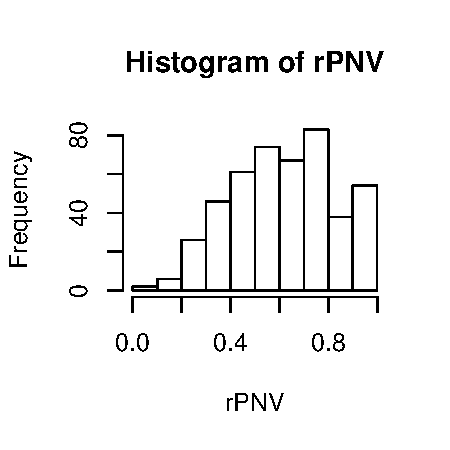
\includegraphics{Landscape_analysis_example_4_files/figure-latex/unnamed-chunk-32-1.pdf}

\#Importerer landskapsegenskapsprofiler fra regneark

\hypertarget{denne-funker-ikke-lep---read.tableclipboardheaderf}{%
\subsubsection{DENNE FUNKER IKKE \#\#\#lep \textless{}-
read.table(``clipboard'',header=F)}\label{denne-funker-ikke-lep---read.tableclipboardheaderf}}

\hypertarget{denne-funker-ikke-attachlep}{%
\subsubsection{DENNE FUNKER IKKE
\#\#\#attach(lep)}\label{denne-funker-ikke-attachlep}}

\hypertarget{denne-funker-ikke-nameslep}{%
\subsubsection{DENNE FUNKER IKKE
\#\#\#names(lep)}\label{denne-funker-ikke-nameslep}}

\hypertarget{denne-funker-ikke-dimlep}{%
\subsubsection{DENNE FUNKER IKKE
\#\#\#dim(lep)}\label{denne-funker-ikke-dimlep}}

\#Beregner artsulikhet (PD)

\hypertarget{denne-funker-ikke-dist---vegdistlepmethodbray}{%
\subsubsection{DENNE FUNKER IKKE \#\#\#dist \textless{}-
vegdist(lep,method=``bray'')}\label{denne-funker-ikke-dist---vegdistlepmethodbray}}

\hypertarget{denne-funker-ikke-dist}{%
\subsubsection{DENNE FUNKER IKKE
\#\#\#dist}\label{denne-funker-ikke-dist}}

\hypertarget{denne-funker-ikke-pd-verdiene-er-s-lave-at-det-ikke-er-noe-behov-for-bruke-geodetisk-avstand}{%
\subsubsection{DENNE FUNKER IKKE \#\#\#\#PD-verdiene er s? lave at det
ikke er noe behov for ? bruke geodetisk
avstand}\label{denne-funker-ikke-pd-verdiene-er-s-lave-at-det-ikke-er-noe-behov-for-bruke-geodetisk-avstand}}

\hypertarget{denne-funker-ikke-eksporterer-til-excel}{%
\subsubsection{DENNE FUNKER IKKE \#\#\#\#Eksporterer til
Excel}\label{denne-funker-ikke-eksporterer-til-excel}}

\hypertarget{denne-funker-ikke-writeclipboardas.characterdist-m-importeres-som-character-jf.-crawley-2007-77}{%
\subsubsection{DENNE FUNKER IKKE
\#\#\#writeClipboard(as.character(dist)) \#M? importeres som `character'
(jf. Crawley 2007:
77)}\label{denne-funker-ikke-writeclipboardas.characterdist-m-importeres-som-character-jf.-crawley-2007-77}}

\hypertarget{denne-funker-ikke-importerer-ia-estimater-fra-nin2lad5oi-pd2}{%
\subsubsection{DENNE FUNKER IKKE \#\#\#\#Importerer IA-estimater fra
NiN2LAD5/OI-PD2}\label{denne-funker-ikke-importerer-ia-estimater-fra-nin2lad5oi-pd2}}

\hypertarget{denne-funker-ikke-iaest.df---read.tableclipboardheadert}{%
\subsubsection{DENNE FUNKER IKKE \#\#\#IAest.df \textless{}-
read.table(``clipboard'',header=T)}\label{denne-funker-ikke-iaest.df---read.tableclipboardheadert}}

\hypertarget{denne-funker-ikke-attachiaest.df}{%
\subsubsection{DENNE FUNKER IKKE
\#\#\#attach(IAest.df)}\label{denne-funker-ikke-attachiaest.df}}

\hypertarget{denne-funker-ikke-namesiaest.df}{%
\subsubsection{DENNE FUNKER IKKE
\#\#\#names(IAest.df)}\label{denne-funker-ikke-namesiaest.df}}

\hypertarget{denne-funker-ikke-histiaest}{%
\subsubsection{DENNE FUNKER IKKE
\#\#\#hist(IAest)}\label{denne-funker-ikke-histiaest}}

\hypertarget{denne-funker-ikke-meaniaest}{%
\subsubsection{DENNE FUNKER IKKE
\#\#\#mean(IAest)}\label{denne-funker-ikke-meaniaest}}

\hypertarget{denne-funker-ikke-sdiaest}{%
\subsubsection{DENNE FUNKER IKKE
\#\#\#sd(IAest)}\label{denne-funker-ikke-sdiaest}}

\hypertarget{finner-primrnkkelvariabler-for-identifiserte-klg-ved-rda-1}{%
\paragraph{Finner prim?rn?kkelvariabler for identifiserte KLG ved
RDA}\label{finner-primrnkkelvariabler-for-identifiserte-klg-ved-rda-1}}

\#Skript for ? finne ortogonale prim?rn?kkelvariabler (rONV'er) i ei
n?kkelvariabelgruppe

\#Om n?dvendig: importerer relevante rPNV'er

\#dta\_pnv \textless{}- read-table(``clipboard'',header=T)
\#attach(dta\_pnv)

\#VE for 1 .akse i RDA'er gir VA(PNV)

\begin{Shaded}
\begin{Highlighting}[]
\KeywordTok{summary}\NormalTok{(oRDA_RE)}\OperatorTok{$}\NormalTok{cont}
\end{Highlighting}
\end{Shaded}

\begin{verbatim}
## $importance
## Importance of components:
##                        RDA1    RDA2     PC1     PC2     PC3     PC4
## Eigenvalue            8.063 2.37481 6.43305 5.39541 3.15314 2.78814
## Proportion Explained  0.116 0.03416 0.09254 0.07761 0.04536 0.04011
## Cumulative Proportion 0.116 0.15015 0.24269 0.32030 0.36566 0.40577
##                           PC5     PC6     PC7    PC8     PC9    PC10
## Eigenvalue            2.34774 2.10420 1.92720 1.6752 1.64141 1.43261
## Proportion Explained  0.03377 0.03027 0.02772 0.0241 0.02361 0.02061
## Cumulative Proportion 0.43954 0.46981 0.49753 0.5216 0.54524 0.56585
##                          PC11    PC12    PC13    PC14    PC15   PC16
## Eigenvalue            1.31029 1.26948 1.22674 1.14618 1.09783 1.0633
## Proportion Explained  0.01885 0.01826 0.01765 0.01649 0.01579 0.0153
## Cumulative Proportion 0.58470 0.60296 0.62060 0.63709 0.65288 0.6682
##                         PC17   PC18    PC19    PC20    PC21   PC22    PC23
## Eigenvalue            1.0357 0.9522 0.94173 0.92072 0.89963 0.8345 0.80145
## Proportion Explained  0.0149 0.0137 0.01355 0.01324 0.01294 0.0120 0.01153
## Cumulative Proportion 0.6831 0.6968 0.71032 0.72357 0.73651 0.7485 0.76004
##                          PC24    PC25    PC26     PC27     PC28     PC29
## Eigenvalue            0.77423 0.73173 0.69305 0.661287 0.653767 0.590749
## Proportion Explained  0.01114 0.01053 0.00997 0.009513 0.009404 0.008498
## Cumulative Proportion 0.77118 0.78171 0.79168 0.801188 0.810593 0.819091
##                           PC30     PC31     PC32     PC33     PC34
## Eigenvalue            0.583993 0.545376 0.531197 0.518277 0.499204
## Proportion Explained  0.008401 0.007845 0.007641 0.007455 0.007181
## Cumulative Proportion 0.827491 0.835337 0.842978 0.850433 0.857614
##                           PC35     PC36     PC37     PC38     PC39
## Eigenvalue            0.492610 0.473827 0.454817 0.438486 0.435580
## Proportion Explained  0.007086 0.006816 0.006543 0.006308 0.006266
## Cumulative Proportion 0.864701 0.871517 0.878059 0.884367 0.890633
##                           PC40     PC41     PC42     PC43     PC44
## Eigenvalue            0.411714 0.381045 0.361901 0.345801 0.341069
## Proportion Explained  0.005923 0.005481 0.005206 0.004974 0.004906
## Cumulative Proportion 0.896555 0.902036 0.907242 0.912217 0.917123
##                           PC45     PC46     PC47     PC48     PC49
## Eigenvalue            0.335224 0.317855 0.312419 0.297112 0.280571
## Proportion Explained  0.004822 0.004572 0.004494 0.004274 0.004036
## Cumulative Proportion 0.921945 0.926518 0.931012 0.935286 0.939322
##                           PC50     PC51     PC52     PC53     PC54
## Eigenvalue            0.274722 0.260070 0.248594 0.230718 0.223554
## Proportion Explained  0.003952 0.003741 0.003576 0.003319 0.003216
## Cumulative Proportion 0.943274 0.947015 0.950591 0.953910 0.957125
##                           PC55     PC56     PC57     PC58     PC59
## Eigenvalue            0.218404 0.213024 0.202581 0.189991 0.178424
## Proportion Explained  0.003142 0.003064 0.002914 0.002733 0.002567
## Cumulative Proportion 0.960267 0.963332 0.966246 0.968979 0.971545
##                           PC60     PC61     PC62     PC63     PC64
## Eigenvalue            0.174154 0.160526 0.154722 0.147461 0.138440
## Proportion Explained  0.002505 0.002309 0.002226 0.002121 0.001991
## Cumulative Proportion 0.974051 0.976360 0.978585 0.980707 0.982698
##                           PC65     PC66     PC67     PC68    PC69     PC70
## Eigenvalue            0.136320 0.126917 0.124902 0.115206 0.11053 0.098668
## Proportion Explained  0.001961 0.001826 0.001797 0.001657 0.00159 0.001419
## Cumulative Proportion 0.984659 0.986485 0.988281 0.989939 0.99153 0.992948
##                           PC71     PC72     PC73      PC74      PC75
## Eigenvalue            0.088719 0.078258 0.069868 0.0656664 0.0594857
## Proportion Explained  0.001276 0.001126 0.001005 0.0009446 0.0008557
## Cumulative Proportion 0.994224 0.995350 0.996355 0.9972997 0.9981554
##                            PC76      PC77      PC78      PC79
## Eigenvalue            0.0466357 0.0421054 0.0226894 0.0168033
## Proportion Explained  0.0006709 0.0006057 0.0003264 0.0002417
## Cumulative Proportion 0.9988262 0.9994319 0.9997583 1.0000000
\end{verbatim}

\begin{Shaded}
\begin{Highlighting}[]
\NormalTok{oRDA_RE <-}\StringTok{ }\KeywordTok{rda}\NormalTok{(av}\OperatorTok{~}\NormalTok{RR1}\OperatorTok{+}\NormalTok{Rug3_m}\OperatorTok{+}\NormalTok{Tpi1h_a,}\DataTypeTok{scale=}\NormalTok{T) }\CommentTok{#er lik PNV, for den f?rst utvalgte gruppa}
\NormalTok{oRDA_SkP <-}\StringTok{ }\KeywordTok{rda}\NormalTok{(av}\OperatorTok{~}\NormalTok{Arbar_a }\OperatorTok{+}\StringTok{ }\NormalTok{Sn_imp}\OperatorTok{+}\KeywordTok{Condition}\NormalTok{(RR1}\OperatorTok{+}\NormalTok{Rug3_m}\OperatorTok{+}\NormalTok{Tpi1h_a),}\DataTypeTok{scale=}\NormalTok{T)}
\NormalTok{oRDA_OI <-}\StringTok{ }\KeywordTok{rda}\NormalTok{(av}\OperatorTok{~}\NormalTok{IfIu}\OperatorTok{+}\NormalTok{Gab_a}\OperatorTok{+}\KeywordTok{Condition}\NormalTok{(Arbar_a }\OperatorTok{+}\StringTok{ }\NormalTok{Sn_imp}\OperatorTok{+}\NormalTok{RR1}\OperatorTok{+}\NormalTok{Rug3_m}\OperatorTok{+}\NormalTok{Tpi1h_a),}\DataTypeTok{scale=}\NormalTok{T)}

\KeywordTok{summary}\NormalTok{(oRDA_RE)}\OperatorTok{$}\NormalTok{cont}
\end{Highlighting}
\end{Shaded}

\begin{verbatim}
## $importance
## Importance of components:
##                         RDA1    RDA2    RDA3     PC1     PC2     PC3
## Eigenvalue            8.7102 3.78332 1.34275 13.5097 6.30468 3.38955
## Proportion Explained  0.1037 0.04504 0.01599  0.1608 0.07506 0.04035
## Cumulative Proportion 0.1037 0.14873 0.16472  0.3255 0.40060 0.44096
##                           PC4     PC5     PC6     PC7     PC8     PC9
## Eigenvalue            2.94935 2.55090 2.38427 2.11766 1.79034 1.68600
## Proportion Explained  0.03511 0.03037 0.02838 0.02521 0.02131 0.02007
## Cumulative Proportion 0.47607 0.50643 0.53482 0.56003 0.58134 0.60141
##                          PC10    PC11    PC12    PC13    PC14    PC15
## Eigenvalue            1.59268 1.46033 1.39092 1.25873 1.17131 1.16590
## Proportion Explained  0.01896 0.01738 0.01656 0.01498 0.01394 0.01388
## Cumulative Proportion 0.62037 0.63776 0.65432 0.66930 0.68325 0.69713
##                          PC16    PC17    PC18    PC19   PC20    PC21
## Eigenvalue            1.14579 1.04939 0.98890 0.96320 0.9238 0.90266
## Proportion Explained  0.01364 0.01249 0.01177 0.01147 0.0110 0.01075
## Cumulative Proportion 0.71077 0.72326 0.73503 0.74650 0.7575 0.76824
##                          PC22     PC23     PC24    PC25     PC26     PC27
## Eigenvalue            0.84973 0.811874 0.792485 0.76103 0.745209 0.710525
## Proportion Explained  0.01012 0.009665 0.009434 0.00906 0.008872 0.008459
## Cumulative Proportion 0.77836 0.788024 0.797458 0.80652 0.815389 0.823848
##                           PC28     PC29     PC30    PC31     PC32     PC33
## Eigenvalue            0.665445 0.629870 0.617724 0.57705 0.561627 0.541607
## Proportion Explained  0.007922 0.007498 0.007354 0.00687 0.006686 0.006448
## Cumulative Proportion 0.831770 0.839268 0.846622 0.85349 0.860178 0.866626
##                          PC34     PC35     PC36     PC37     PC38     PC39
## Eigenvalue            0.52332 0.492371 0.483081 0.475508 0.460711 0.446778
## Proportion Explained  0.00623 0.005862 0.005751 0.005661 0.005485 0.005319
## Cumulative Proportion 0.87286 0.878717 0.884468 0.890129 0.895614 0.900932
##                           PC40     PC41     PC42     PC43    PC44     PC45
## Eigenvalue            0.433323 0.409604 0.382562 0.373022 0.35781 0.354361
## Proportion Explained  0.005159 0.004876 0.004554 0.004441 0.00426 0.004219
## Cumulative Proportion 0.906091 0.910967 0.915522 0.919962 0.92422 0.928441
##                           PC46     PC47     PC48     PC49     PC50
## Eigenvalue            0.331915 0.323960 0.315356 0.294458 0.280459
## Proportion Explained  0.003951 0.003857 0.003754 0.003505 0.003339
## Cumulative Proportion 0.932392 0.936249 0.940003 0.943508 0.946847
##                           PC51     PC52     PC53     PC54     PC55
## Eigenvalue            0.274269 0.260823 0.240439 0.232470 0.226153
## Proportion Explained  0.003265 0.003105 0.002862 0.002768 0.002692
## Cumulative Proportion 0.950112 0.953217 0.956080 0.958847 0.961539
##                           PC56     PC57     PC58     PC59     PC60
## Eigenvalue            0.219930 0.208229 0.197655 0.190421 0.187433
## Proportion Explained  0.002618 0.002479 0.002353 0.002267 0.002231
## Cumulative Proportion 0.964158 0.966636 0.968990 0.971256 0.973488
##                           PC61    PC62     PC63     PC64     PC65     PC66
## Eigenvalue            0.179375 0.16715 0.158444 0.151468 0.147476 0.143002
## Proportion Explained  0.002135 0.00199 0.001886 0.001803 0.001756 0.001702
## Cumulative Proportion 0.975623 0.97761 0.979499 0.981303 0.983058 0.984761
##                           PC67     PC68    PC69     PC70     PC71     PC72
## Eigenvalue            0.135980 0.129659 0.12266 0.117275 0.113045 0.108547
## Proportion Explained  0.001619 0.001544 0.00146 0.001396 0.001346 0.001292
## Cumulative Proportion 0.986379 0.987923 0.98938 0.990779 0.992125 0.993417
##                           PC73     PC74      PC75      PC76      PC77
## Eigenvalue            0.096128 0.086432 0.0780087 0.0684356 0.0653167
## Proportion Explained  0.001144 0.001029 0.0009287 0.0008147 0.0007776
## Cumulative Proportion 0.994562 0.995591 0.9965193 0.9973341 0.9981116
##                            PC78      PC79      PC80      PC81      PC82
## Eigenvalue            0.0548579 0.0422310 0.0281821 0.0201686 0.0131827
## Proportion Explained  0.0006531 0.0005028 0.0003355 0.0002401 0.0001569
## Cumulative Proportion 0.9987647 0.9992675 0.9996030 0.9998431 1.0000000
\end{verbatim}

\begin{Shaded}
\begin{Highlighting}[]
\KeywordTok{summary}\NormalTok{(oRDA_SkP)}\OperatorTok{$}\NormalTok{cont }\CommentTok{#gir aksenes egenverdier}
\end{Highlighting}
\end{Shaded}

\begin{verbatim}
## $importance
## Importance of components:
##                         RDA1    RDA2     PC1     PC2     PC3     PC4
## Eigenvalue            8.9390 1.20325 6.77667 5.47575 3.31767 2.83062
## Proportion Explained  0.1274 0.01715 0.09658 0.07804 0.04728 0.04034
## Cumulative Proportion 0.1274 0.14455 0.24113 0.31918 0.36646 0.40681
##                           PC5     PC6     PC7     PC8    PC9    PC10
## Eigenvalue            2.30444 2.12750 2.03828 1.68625 1.5856 1.46066
## Proportion Explained  0.03284 0.03032 0.02905 0.02403 0.0226 0.02082
## Cumulative Proportion 0.43965 0.46997 0.49902 0.52305 0.5457 0.56647
##                          PC11    PC12    PC13    PC14    PC15    PC16
## Eigenvalue            1.38082 1.34406 1.24494 1.16362 1.09643 1.04900
## Proportion Explained  0.01968 0.01916 0.01774 0.01658 0.01563 0.01495
## Cumulative Proportion 0.58615 0.60531 0.62305 0.63963 0.65526 0.67021
##                          PC17    PC18    PC19    PC20    PC21    PC22
## Eigenvalue            0.98531 0.96367 0.94300 0.88805 0.86713 0.82157
## Proportion Explained  0.01404 0.01373 0.01344 0.01266 0.01236 0.01171
## Cumulative Proportion 0.68426 0.69799 0.71143 0.72409 0.73645 0.74815
##                          PC23    PC24   PC25    PC26     PC27     PC28
## Eigenvalue            0.80593 0.76707 0.7440 0.71347 0.678565 0.651782
## Proportion Explained  0.01149 0.01093 0.0106 0.01017 0.009671 0.009289
## Cumulative Proportion 0.75964 0.77057 0.7812 0.79135 0.801017 0.810306
##                          PC29     PC30     PC31     PC32     PC33     PC34
## Eigenvalue            0.62304 0.582639 0.572250 0.537977 0.521086 0.500052
## Proportion Explained  0.00888 0.008304 0.008156 0.007667 0.007427 0.007127
## Cumulative Proportion 0.81919 0.827490 0.835646 0.843313 0.850740 0.857867
##                           PC35     PC36     PC37     PC38     PC39
## Eigenvalue            0.485194 0.476290 0.464695 0.441028 0.415464
## Proportion Explained  0.006915 0.006788 0.006623 0.006286 0.005921
## Cumulative Proportion 0.864782 0.871570 0.878194 0.884479 0.890401
##                           PC40     PC41     PC42     PC43     PC44
## Eigenvalue            0.395974 0.378398 0.367480 0.358710 0.344298
## Proportion Explained  0.005644 0.005393 0.005237 0.005112 0.004907
## Cumulative Proportion 0.896044 0.901437 0.906675 0.911787 0.916694
##                           PC45     PC46     PC47     PC48     PC49
## Eigenvalue            0.325728 0.321075 0.309777 0.298001 0.279212
## Proportion Explained  0.004642 0.004576 0.004415 0.004247 0.003979
## Cumulative Proportion 0.921337 0.925913 0.930328 0.934575 0.938554
##                           PC50     PC51     PC52     PC53     PC54
## Eigenvalue            0.274084 0.260089 0.240556 0.231931 0.226232
## Proportion Explained  0.003906 0.003707 0.003428 0.003306 0.003224
## Cumulative Proportion 0.942461 0.946168 0.949596 0.952902 0.956126
##                           PC55     PC56   PC57     PC58     PC59     PC60
## Eigenvalue            0.218445 0.210618 0.1964 0.188690 0.186355 0.168145
## Proportion Explained  0.003113 0.003002 0.0028 0.002689 0.002656 0.002396
## Cumulative Proportion 0.959239 0.962241 0.9650 0.967730 0.970386 0.972783
##                           PC61     PC62     PC63     PC64    PC65     PC66
## Eigenvalue            0.167084 0.152082 0.149199 0.145159 0.14172 0.131674
## Proportion Explained  0.002381 0.002168 0.002126 0.002069 0.00202 0.001877
## Cumulative Proportion 0.975164 0.977332 0.979458 0.981527 0.98355 0.985423
##                           PC67     PC68     PC69     PC70     PC71
## Eigenvalue            0.125841 0.117415 0.113357 0.108551 0.096571
## Proportion Explained  0.001794 0.001673 0.001616 0.001547 0.001376
## Cumulative Proportion 0.987217 0.988890 0.990506 0.992053 0.993429
##                           PC72     PC73      PC74      PC75      PC76
## Eigenvalue            0.089639 0.078544 0.0685229 0.0655213 0.0549459
## Proportion Explained  0.001278 0.001119 0.0009766 0.0009338 0.0007831
## Cumulative Proportion 0.994707 0.995826 0.9968030 0.9977368 0.9985199
##                            PC77      PC78      PC79     PC80
## Eigenvalue            0.0422652 0.0282169 0.0201742 0.013190
## Proportion Explained  0.0006024 0.0004022 0.0002875 0.000188
## Cumulative Proportion 0.9991223 0.9995245 0.9998120 1.000000
\end{verbatim}

\begin{Shaded}
\begin{Highlighting}[]
\KeywordTok{summary}\NormalTok{(oRDA_OI)}\OperatorTok{$}\NormalTok{cont}
\end{Highlighting}
\end{Shaded}

\begin{verbatim}
## $importance
## Importance of components:
##                          RDA1    RDA2     PC1     PC2     PC3     PC4
## Eigenvalue            4.31384 1.85098 5.73975 3.48573 2.61238 2.30324
## Proportion Explained  0.07187 0.03084 0.09563 0.05807 0.04352 0.03837
## Cumulative Proportion 0.07187 0.10271 0.19834 0.25641 0.29994 0.33831
##                           PC5    PC6     PC7     PC8     PC9    PC10
## Eigenvalue            2.04870 1.9985 1.77524 1.60334 1.57608 1.45048
## Proportion Explained  0.03413 0.0333 0.02958 0.02671 0.02626 0.02417
## Cumulative Proportion 0.37244 0.4057 0.43532 0.46203 0.48829 0.51245
##                          PC11    PC12    PC13    PC14    PC15    PC16
## Eigenvalue            1.34323 1.25311 1.17877 1.10503 1.02925 0.98964
## Proportion Explained  0.02238 0.02088 0.01964 0.01841 0.01715 0.01649
## Cumulative Proportion 0.53483 0.55571 0.57535 0.59376 0.61091 0.62740
##                         PC17    PC18    PC19    PC20    PC21    PC22
## Eigenvalue            0.9661 0.93971 0.89610 0.85929 0.83914 0.78660
## Proportion Explained  0.0161 0.01566 0.01493 0.01432 0.01398 0.01311
## Cumulative Proportion 0.6435 0.65915 0.67408 0.68839 0.70237 0.71548
##                         PC23    PC24    PC25   PC26    PC27    PC28
## Eigenvalue            0.7621 0.74834 0.70739 0.7023 0.66711 0.61979
## Proportion Explained  0.0127 0.01247 0.01179 0.0117 0.01111 0.01033
## Cumulative Proportion 0.7282 0.74065 0.75243 0.7641 0.77525 0.78557
##                           PC29     PC30     PC31     PC32     PC33
## Eigenvalue            0.586142 0.564683 0.545155 0.537542 0.503326
## Proportion Explained  0.009766 0.009408 0.009083 0.008956 0.008386
## Cumulative Proportion 0.795339 0.804747 0.813829 0.822785 0.831171
##                           PC34     PC35     PC36     PC37     PC38
## Eigenvalue            0.498135 0.479134 0.462126 0.451631 0.416848
## Proportion Explained  0.008299 0.007983 0.007699 0.007524 0.006945
## Cumulative Proportion 0.839470 0.847453 0.855152 0.862677 0.869622
##                           PC39     PC40     PC41     PC42     PC43
## Eigenvalue            0.399445 0.382096 0.376505 0.365382 0.343990
## Proportion Explained  0.006655 0.006366 0.006273 0.006088 0.005731
## Cumulative Proportion 0.876277 0.882643 0.888916 0.895003 0.900734
##                           PC44    PC45     PC46     PC47     PC48     PC49
## Eigenvalue            0.329591 0.32169 0.310089 0.303066 0.285195 0.273762
## Proportion Explained  0.005491 0.00536 0.005166 0.005049 0.004752 0.004561
## Cumulative Proportion 0.906226 0.91159 0.916752 0.921801 0.926552 0.931113
##                           PC50     PC51     PC52     PC53     PC54
## Eigenvalue            0.269112 0.250927 0.235079 0.229638 0.218197
## Proportion Explained  0.004484 0.004181 0.003917 0.003826 0.003635
## Cumulative Proportion 0.935597 0.939778 0.943694 0.947520 0.951156
##                           PC55     PC56     PC57     PC58     PC59
## Eigenvalue            0.211077 0.206916 0.190224 0.185393 0.171731
## Proportion Explained  0.003517 0.003447 0.003169 0.003089 0.002861
## Cumulative Proportion 0.954672 0.958120 0.961289 0.964378 0.967239
##                           PC60     PC61     PC62    PC63    PC64     PC65
## Eigenvalue            0.162924 0.160546 0.152069 0.14706 0.14283 0.135966
## Proportion Explained  0.002714 0.002675 0.002534 0.00245 0.00238 0.002265
## Cumulative Proportion 0.969953 0.972628 0.975162 0.97761 0.97999 0.982257
##                           PC66     PC67     PC68     PC69     PC70
## Eigenvalue            0.125364 0.124610 0.115983 0.112789 0.108457
## Proportion Explained  0.002089 0.002076 0.001932 0.001879 0.001807
## Cumulative Proportion 0.984345 0.986421 0.988354 0.990233 0.992040
##                           PC71     PC72     PC73     PC74      PC75
## Eigenvalue            0.095962 0.087299 0.071016 0.064382 0.0550785
## Proportion Explained  0.001599 0.001454 0.001183 0.001073 0.0009176
## Cumulative Proportion 0.993639 0.995093 0.996276 0.997349 0.9982666
##                            PC76      PC77      PC78      PC79
## Eigenvalue            0.0423860 0.0282867 0.0202033 0.0131623
## Proportion Explained  0.0007062 0.0004713 0.0003366 0.0002193
## Cumulative Proportion 0.9989728 0.9994441 0.9997807 1.0000000
\end{verbatim}

\begin{Shaded}
\begin{Highlighting}[]
\CommentTok{#Ekstraksjon av ONV; dette er vektorer}
\NormalTok{ONV_RE <-}\StringTok{ }\KeywordTok{scores}\NormalTok{(oRDA_RE, }\DataTypeTok{display=}\StringTok{"lc"}\NormalTok{, }\DataTypeTok{choices=}\DecValTok{1}\NormalTok{, }\DataTypeTok{scaling=}\DecValTok{1}\NormalTok{)}
\NormalTok{ONV_SkP <-}\StringTok{ }\OperatorTok{-}\KeywordTok{scores}\NormalTok{(oRDA_SkP, }\DataTypeTok{display=}\StringTok{"lc"}\NormalTok{, }\DataTypeTok{choices=}\DecValTok{1}\NormalTok{, }\DataTypeTok{scaling=}\DecValTok{1}\NormalTok{)}
\NormalTok{ONV_OI <-}\StringTok{ }\OperatorTok{-}\KeywordTok{scores}\NormalTok{(oRDA_OI, }\DataTypeTok{display=}\StringTok{"lc"}\NormalTok{, }\DataTypeTok{choices=}\DecValTok{1}\NormalTok{, }\DataTypeTok{scaling=}\DecValTok{1}\NormalTok{)}
\end{Highlighting}
\end{Shaded}

\begin{Shaded}
\begin{Highlighting}[]
\CommentTok{#Sjekker om rONV'en har samme fortegn som variablen(e) som karakteriserer den, og gjlrb om n?dvendig ny ekstraksjon av sk?rer med motsatt fortegn}
\KeywordTok{cor.test}\NormalTok{(ONV_RE,Rr1_m,}\DataTypeTok{method=}\StringTok{"k"}\NormalTok{)}
\end{Highlighting}
\end{Shaded}

\begin{verbatim}
## 
##  Kendall's rank correlation tau
## 
## data:  ONV_RE and Rr1_m
## z = -24.492, p-value < 2.2e-16
## alternative hypothesis: true tau is not equal to 0
## sample estimates:
##        tau 
## -0.7690107
\end{verbatim}

\begin{Shaded}
\begin{Highlighting}[]
\KeywordTok{cor.test}\NormalTok{(ONV_SkP,Arbar_a,}\DataTypeTok{method=}\StringTok{"k"}\NormalTok{)}
\end{Highlighting}
\end{Shaded}

\begin{verbatim}
## 
##  Kendall's rank correlation tau
## 
## data:  ONV_SkP and Arbar_a
## z = -23.904, p-value < 2.2e-16
## alternative hypothesis: true tau is not equal to 0
## sample estimates:
##        tau 
## -0.7881209
\end{verbatim}

\begin{Shaded}
\begin{Highlighting}[]
\KeywordTok{cor.test}\NormalTok{(ONV_OI,IfIu,}\DataTypeTok{method=}\StringTok{"k"}\NormalTok{)}
\end{Highlighting}
\end{Shaded}

\begin{verbatim}
## 
##  Kendall's rank correlation tau
## 
## data:  ONV_OI and IfIu
## z = 14.704, p-value < 2.2e-16
## alternative hypothesis: true tau is not equal to 0
## sample estimates:
##       tau 
## 0.4650136
\end{verbatim}

\#Eksporterer evt sk?rer langs ONV'ene til Excel
writeClipboard(as.character(ONV\_RE))
writeClipboard(as.character(ONV\_SkP))
writeClipboard(as.character(ONV\_OI))

\begin{Shaded}
\begin{Highlighting}[]
\CommentTok{#Rangerer ONV'ene}

\NormalTok{rONV_RE <-}\StringTok{ }\NormalTok{(ONV_RE}\OperatorTok{-}\KeywordTok{min}\NormalTok{(ONV_RE))}\OperatorTok{/}\NormalTok{(}\KeywordTok{max}\NormalTok{(ONV_RE)}\OperatorTok{-}\KeywordTok{min}\NormalTok{(ONV_RE)) }\CommentTok{#Tar vare p? de korrigerte prim?rn?kkelvariablene}
\NormalTok{rONV_SkP <-}\StringTok{ }\NormalTok{(ONV_SkP}\OperatorTok{-}\KeywordTok{min}\NormalTok{(ONV_SkP))}\OperatorTok{/}\NormalTok{(}\KeywordTok{max}\NormalTok{(ONV_SkP)}\OperatorTok{-}\KeywordTok{min}\NormalTok{(ONV_SkP))}
\NormalTok{rONV_OI <-}\StringTok{ }\NormalTok{(ONV_OI}\OperatorTok{-}\KeywordTok{min}\NormalTok{(ONV_OI))}\OperatorTok{/}\NormalTok{(}\KeywordTok{max}\NormalTok{(ONV_OI)}\OperatorTok{-}\KeywordTok{min}\NormalTok{(ONV_OI))}
\end{Highlighting}
\end{Shaded}

\#Eksporterer rONV-sk?rer til Excel

writeClipboard(as.character(rONV\_RE))
writeClipboard(as.character(rONV\_SkP))
writeClipboard(as.character(rONV\_OI))

\hypertarget{beregning-av-la-mellom-klg-klasser-ved-bruk-av-pd-1}{%
\paragraph{Beregning av LA mellom KLG-klasser ved bruk av
PD}\label{beregning-av-la-mellom-klg-klasser-ved-bruk-av-pd-1}}

\#Importerer om n?dvendig rPNVer fra Excel:

\#rPNV \textless{}- read.table(``clipboard'',header=T) \#attach(rPNV)
\#names(rPNV)

\#Analyse av KLG'er representert ved rangerte n?kkelvariabler

\begin{Shaded}
\begin{Highlighting}[]
\NormalTok{rONV <-}\StringTok{ }\NormalTok{rONV_OI}

\CommentTok{#Inspeksjon av OE'enes frekvensfordeling langs rPNV'en}
\KeywordTok{hist}\NormalTok{(rONV)}
\end{Highlighting}
\end{Shaded}

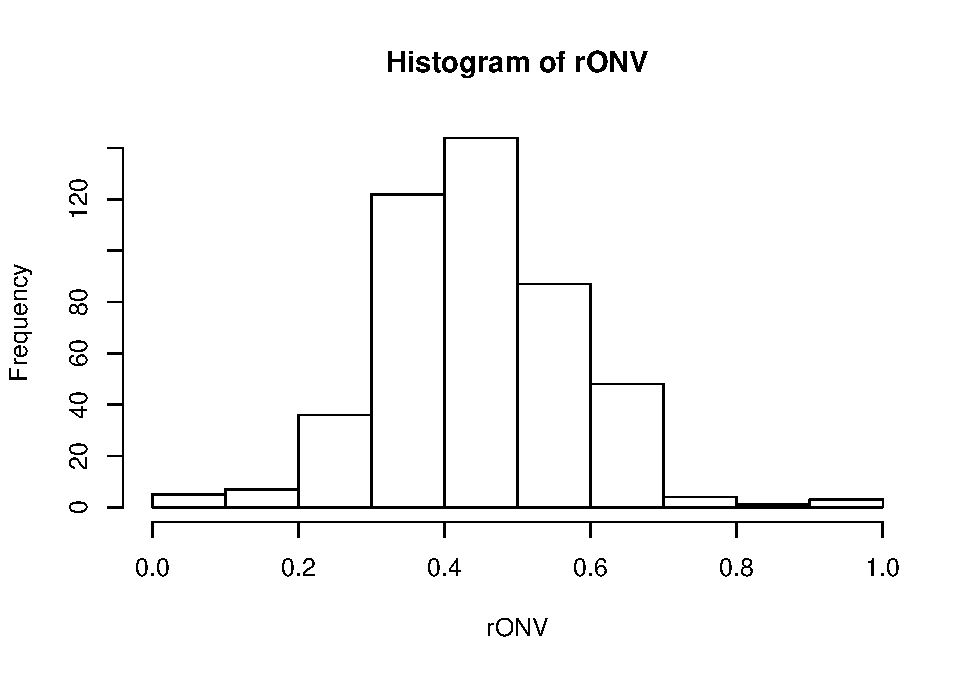
\includegraphics{Landscape_analysis_example_4_files/figure-latex/unnamed-chunk-39-1.pdf}

\#Importerer landskapsegenskapsprofiler fra regneark \#\#\# DENNE FUNKER
IKKE \#\#\# \#\#\# DENNE FUNKER IKKE \#\#\# lep \textless{}-
read.table(``clipboard'',header=F) \#\#\# DENNE FUNKER IKKE \#\#\#lep
\textless{}- as.numeric(lep) \#\#\# DENNE FUNKER IKKE \#\#\#attach(lep)
\#\#\# DENNE FUNKER IKKE \#\#\#names(lep)

\hypertarget{denne-funker-ikke-dimlep-1}{%
\subsubsection{DENNE FUNKER IKKE
\#\#\#dim(lep)}\label{denne-funker-ikke-dimlep-1}}

\hypertarget{denne-funker-ikke-beregner-artsulikhet-pd}{%
\subsubsection{DENNE FUNKER IKKE \#\#\#\#Beregner artsulikhet
(PD)}\label{denne-funker-ikke-beregner-artsulikhet-pd}}

\hypertarget{denne-funker-ikke-dist---vegdistlepmethodbray-1}{%
\subsubsection{DENNE FUNKER IKKE \#\#\#dist \textless{}-
vegdist(lep,method=``bray'')}\label{denne-funker-ikke-dist---vegdistlepmethodbray-1}}

\hypertarget{denne-funker-ikke-dist-1}{%
\subsubsection{DENNE FUNKER IKKE
\#\#\#dist}\label{denne-funker-ikke-dist-1}}

\hypertarget{denne-funker-ikke-pd-verdiene-er-s-lave-at-det-ikke-er-noe-behov-for-bruke-geodetisk-avstand-1}{%
\subsubsection{DENNE FUNKER IKKE \#\#\#\#PD-verdiene er s? lave at det
ikke er noe behov for ? bruke geodetisk
avstand}\label{denne-funker-ikke-pd-verdiene-er-s-lave-at-det-ikke-er-noe-behov-for-bruke-geodetisk-avstand-1}}

\hypertarget{denne-funker-ikke-eksporterer-til-excel-1}{%
\subsubsection{DENNE FUNKER IKKE \#\#\#\#Eksporterer til
Excel}\label{denne-funker-ikke-eksporterer-til-excel-1}}

\hypertarget{denne-funker-ikke-writeclipboardas.characterdist-m-importeres-som-character-jf.-crawley-2007-77-1}{%
\subsubsection{DENNE FUNKER IKKE
\#\#\#writeClipboard(as.character(dist)) \#M? importeres som `character'
(jf. Crawley 2007:
77)}\label{denne-funker-ikke-writeclipboardas.characterdist-m-importeres-som-character-jf.-crawley-2007-77-1}}

\hypertarget{denne-funker-ikke-cor.testifiuronv_ap}{%
\subsubsection{DENNE FUNKER IKKE
\#\#\#cor.test(IfIu,rONV\_AP)}\label{denne-funker-ikke-cor.testifiuronv_ap}}

\hypertarget{denne-funker-ikke-slutt}{%
\subsubsection{DENNE FUNKER IKKE \#\#\#
SLUTT}\label{denne-funker-ikke-slutt}}

\hypertarget{analyser-av-samvariasjon-mellom-reskalerte-ronver-sonv}{%
\paragraph{Analyser av samvariasjon mellom reskalerte rONV'er
(sONV)}\label{analyser-av-samvariasjon-mellom-reskalerte-ronver-sonv}}

\#Fig. 1. 1 IyK mot 2 RE; SN som symboler og isolinjer for Oyst\_i

\begin{Shaded}
\begin{Highlighting}[]
\CommentTok{#sONV'er som skal plottes mot hverandre}
\NormalTok{s1 <-}\StringTok{ }\NormalTok{sONV_IyK}
\NormalTok{s2 <-}\StringTok{ }\NormalTok{sONV_RE}
\end{Highlighting}
\end{Shaded}

\#Finner koordinatene for hj?rner i det `plotteomr?det' med koordinater
(x1, x2, y1, y2) som gir \#like enheter p? begge akser. Vi holder x1, x2
og y1 faste og bestemmer y2 slik at (x2-x1)/(y2-y1) i plt=c(x1,x2,y1,y2)
\#blir lik max(s1)/max(s2) \#Det krever at y2 = {[}(x2-x1)\emph{max(s2)
+ y1}max(s1){]}/max(s1) \#Setter vi x1, x2 og y1 konstante, f?r vi:

\begin{Shaded}
\begin{Highlighting}[]
\NormalTok{y2 <-}\StringTok{ }\NormalTok{(}\FloatTok{0.8}\OperatorTok{*}\KeywordTok{max}\NormalTok{(s2)}\OperatorTok{+}\FloatTok{0.15}\OperatorTok{*}\KeywordTok{max}\NormalTok{(s1))}\OperatorTok{/}\KeywordTok{max}\NormalTok{(s1)}
\NormalTok{y2}
\end{Highlighting}
\end{Shaded}

\begin{verbatim}
## [1] 0.7467213
\end{verbatim}

\begin{Shaded}
\begin{Highlighting}[]
\CommentTok{#Plotter SN-klasser p? figuren, og legger p? isolinjer for Oyst_i}
\KeywordTok{par}\NormalTok{(}\DataTypeTok{plt=}\KeywordTok{c}\NormalTok{(}\FloatTok{0.15}\NormalTok{, }\FloatTok{0.95}\NormalTok{, }\FloatTok{0.15}\NormalTok{, y2))}
\KeywordTok{plot}\NormalTok{(s1,s2,}\DataTypeTok{xlab=}\StringTok{"KLG 1 IYF - Coastal plains (KS457)"}\NormalTok{,}\DataTypeTok{ylab=}\StringTok{"KLG 2 RE - Coastal plains (KS457)"}\NormalTok{,}\DataTypeTok{xlim=}\KeywordTok{c}\NormalTok{(}\OperatorTok{-}\FloatTok{0.01}\NormalTok{,}\KeywordTok{max}\NormalTok{(s1)}\OperatorTok{+}\FloatTok{0.01}\NormalTok{),}\DataTypeTok{ylim=}\KeywordTok{c}\NormalTok{(}\OperatorTok{-}\FloatTok{0.01}\NormalTok{,}\KeywordTok{max}\NormalTok{(s2)}\OperatorTok{+}\FloatTok{0.01}\NormalTok{),}\DataTypeTok{xaxp=}\KeywordTok{c}\NormalTok{(}\DecValTok{0}\NormalTok{,}\FloatTok{0.4}\NormalTok{,}\DecValTok{5}\NormalTok{),}\DataTypeTok{yaxp=}\KeywordTok{c}\NormalTok{(}\DecValTok{0}\NormalTok{,}\FloatTok{0.4}\NormalTok{,}\DecValTok{5}\NormalTok{),}\DataTypeTok{type=}\StringTok{"n"}\NormalTok{) }\CommentTok{#Grunnlag for plotting av symboler etc.}
\KeywordTok{lines}\NormalTok{(}\KeywordTok{c}\NormalTok{(}\DecValTok{0}\NormalTok{,}\KeywordTok{max}\NormalTok{(s1)),}\KeywordTok{c}\NormalTok{(}\KeywordTok{max}\NormalTok{(s2),}\KeywordTok{max}\NormalTok{(s2)),}\DataTypeTok{lty=}\DecValTok{3}\NormalTok{,}\DataTypeTok{col=}\DecValTok{8}\NormalTok{)}
\KeywordTok{lines}\NormalTok{(}\KeywordTok{c}\NormalTok{(}\DecValTok{0}\NormalTok{,}\KeywordTok{max}\NormalTok{(s1)),}\KeywordTok{c}\NormalTok{(}\DecValTok{0}\NormalTok{,}\DecValTok{0}\NormalTok{),}\DataTypeTok{lty=}\DecValTok{3}\NormalTok{,}\DataTypeTok{col=}\DecValTok{8}\NormalTok{)}
\KeywordTok{lines}\NormalTok{(}\KeywordTok{c}\NormalTok{(}\DecValTok{0}\NormalTok{,}\DecValTok{0}\NormalTok{),}\KeywordTok{c}\NormalTok{(}\DecValTok{0}\NormalTok{,}\KeywordTok{max}\NormalTok{(s2)),}\DataTypeTok{lty=}\DecValTok{3}\NormalTok{,}\DataTypeTok{col=}\DecValTok{8}\NormalTok{)}
\KeywordTok{lines}\NormalTok{(}\KeywordTok{c}\NormalTok{(}\KeywordTok{max}\NormalTok{(s1),}\KeywordTok{max}\NormalTok{(s1)),}\KeywordTok{c}\NormalTok{(}\DecValTok{0}\NormalTok{,}\KeywordTok{max}\NormalTok{(s2)),}\DataTypeTok{lty=}\DecValTok{3}\NormalTok{,}\DataTypeTok{col=}\DecValTok{8}\NormalTok{)}

\KeywordTok{lines}\NormalTok{(}\KeywordTok{c}\NormalTok{(}\DecValTok{0}\NormalTok{,}\KeywordTok{max}\NormalTok{(s1)),}\KeywordTok{c}\NormalTok{(}\KeywordTok{max}\NormalTok{(s2)}\OperatorTok{/}\DecValTok{3}\NormalTok{,}\KeywordTok{max}\NormalTok{(s2)}\OperatorTok{/}\DecValTok{3}\NormalTok{),}\DataTypeTok{lty=}\DecValTok{2}\NormalTok{,}\DataTypeTok{col=}\DecValTok{8}\NormalTok{)}
\KeywordTok{lines}\NormalTok{(}\KeywordTok{c}\NormalTok{(}\DecValTok{0}\NormalTok{,}\KeywordTok{max}\NormalTok{(s1)),}\KeywordTok{c}\NormalTok{(}\DecValTok{2}\OperatorTok{*}\KeywordTok{max}\NormalTok{(s2)}\OperatorTok{/}\DecValTok{3}\NormalTok{,}\DecValTok{2}\OperatorTok{*}\KeywordTok{max}\NormalTok{(s2)}\OperatorTok{/}\DecValTok{3}\NormalTok{),}\DataTypeTok{lty=}\DecValTok{3}\NormalTok{,}\DataTypeTok{col=}\DecValTok{8}\NormalTok{)}
\KeywordTok{lines}\NormalTok{(}\KeywordTok{c}\NormalTok{(}\FloatTok{0.2}\OperatorTok{*}\KeywordTok{max}\NormalTok{(s1),}\FloatTok{0.2}\OperatorTok{*}\KeywordTok{max}\NormalTok{(s1)),}\KeywordTok{c}\NormalTok{(}\DecValTok{0}\NormalTok{,}\KeywordTok{max}\NormalTok{(s2)}\OperatorTok{-}\FloatTok{0.025}\NormalTok{),}\DataTypeTok{lty=}\DecValTok{2}\NormalTok{,}\DataTypeTok{col=}\DecValTok{8}\NormalTok{)}
\KeywordTok{lines}\NormalTok{(}\KeywordTok{c}\NormalTok{(}\FloatTok{0.4}\OperatorTok{*}\KeywordTok{max}\NormalTok{(s1),}\FloatTok{0.4}\OperatorTok{*}\KeywordTok{max}\NormalTok{(s1)),}\KeywordTok{c}\NormalTok{(}\DecValTok{0}\NormalTok{,}\KeywordTok{max}\NormalTok{(s2)),}\DataTypeTok{lty=}\DecValTok{2}\NormalTok{,}\DataTypeTok{col=}\DecValTok{8}\NormalTok{)}
\KeywordTok{lines}\NormalTok{(}\KeywordTok{c}\NormalTok{(}\FloatTok{0.6}\OperatorTok{*}\KeywordTok{max}\NormalTok{(s1),}\FloatTok{0.6}\OperatorTok{*}\KeywordTok{max}\NormalTok{(s1)),}\KeywordTok{c}\NormalTok{(}\DecValTok{0}\NormalTok{,}\KeywordTok{max}\NormalTok{(s2)),}\DataTypeTok{lty=}\DecValTok{2}\NormalTok{,}\DataTypeTok{col=}\DecValTok{8}\NormalTok{)}
\KeywordTok{lines}\NormalTok{(}\KeywordTok{c}\NormalTok{(}\FloatTok{0.8}\OperatorTok{*}\KeywordTok{max}\NormalTok{(s1),}\FloatTok{0.8}\OperatorTok{*}\KeywordTok{max}\NormalTok{(s1)),}\KeywordTok{c}\NormalTok{(}\DecValTok{0}\NormalTok{,}\KeywordTok{max}\NormalTok{(s2)),}\DataTypeTok{lty=}\DecValTok{2}\NormalTok{,}\DataTypeTok{col=}\DecValTok{8}\NormalTok{)}

\KeywordTok{lines}\NormalTok{(}\KeywordTok{c}\NormalTok{(}\DecValTok{0}\NormalTok{,}\FloatTok{0.142}\NormalTok{),}\KeywordTok{c}\NormalTok{(}\KeywordTok{max}\NormalTok{(s2),}\KeywordTok{max}\NormalTok{(s2)),}\DataTypeTok{col=}\DecValTok{8}\NormalTok{)}
\KeywordTok{lines}\NormalTok{(}\KeywordTok{c}\NormalTok{(}\DecValTok{0}\NormalTok{,}\FloatTok{0.142}\NormalTok{),}\KeywordTok{c}\NormalTok{(}\KeywordTok{max}\NormalTok{(s2)}\OperatorTok{-}\FloatTok{0.025}\NormalTok{,}\KeywordTok{max}\NormalTok{(s2)}\OperatorTok{-}\FloatTok{0.025}\NormalTok{),}\DataTypeTok{col=}\DecValTok{8}\NormalTok{)}
\KeywordTok{lines}\NormalTok{(}\KeywordTok{c}\NormalTok{(}\FloatTok{0.142}\NormalTok{,}\FloatTok{0.142}\NormalTok{),}\KeywordTok{c}\NormalTok{(}\KeywordTok{max}\NormalTok{(s2)}\OperatorTok{-}\FloatTok{0.025}\NormalTok{,}\KeywordTok{max}\NormalTok{(s2)),}\DataTypeTok{col=}\DecValTok{8}\NormalTok{)}
\KeywordTok{lines}\NormalTok{(}\KeywordTok{c}\NormalTok{(}\DecValTok{0}\NormalTok{,}\DecValTok{0}\NormalTok{),}\KeywordTok{c}\NormalTok{(}\KeywordTok{max}\NormalTok{(s2)}\OperatorTok{-}\FloatTok{0.025}\NormalTok{,}\KeywordTok{max}\NormalTok{(s2)),}\DataTypeTok{col=}\DecValTok{8}\NormalTok{)}
\KeywordTok{points}\NormalTok{(}\FloatTok{0.01}\NormalTok{,}\KeywordTok{max}\NormalTok{(s2)}\OperatorTok{-}\FloatTok{0.012}\NormalTok{,}\DataTypeTok{pch=}\DecValTok{16}\NormalTok{,}\DataTypeTok{cex=}\FloatTok{0.5}\NormalTok{,}\DataTypeTok{col=}\StringTok{"black"}\NormalTok{)}
\KeywordTok{points}\NormalTok{(}\FloatTok{0.02}\NormalTok{,}\KeywordTok{max}\NormalTok{(s2)}\OperatorTok{-}\FloatTok{0.012}\NormalTok{,}\DataTypeTok{pch=}\DecValTok{16}\NormalTok{,}\DataTypeTok{cex=}\FloatTok{0.6}\NormalTok{,}\DataTypeTok{col=}\StringTok{"lightblue2"}\NormalTok{)}
\KeywordTok{points}\NormalTok{(}\FloatTok{0.03}\NormalTok{,}\KeywordTok{max}\NormalTok{(s2)}\OperatorTok{-}\FloatTok{0.012}\NormalTok{,}\DataTypeTok{pch=}\DecValTok{16}\NormalTok{,}\DataTypeTok{cex=}\FloatTok{0.75}\NormalTok{,}\DataTypeTok{col=}\StringTok{"darkblue"}\NormalTok{)}
\KeywordTok{points}\NormalTok{(}\FloatTok{0.04}\NormalTok{,}\KeywordTok{max}\NormalTok{(s2)}\OperatorTok{-}\FloatTok{0.012}\NormalTok{,}\DataTypeTok{pch=}\DecValTok{1}\NormalTok{,}\DataTypeTok{cex=}\FloatTok{0.75}\NormalTok{,}\DataTypeTok{col=}\StringTok{"red"}\NormalTok{)}
\KeywordTok{points}\NormalTok{(}\FloatTok{0.05}\NormalTok{,}\KeywordTok{max}\NormalTok{(s2)}\OperatorTok{-}\FloatTok{0.012}\NormalTok{,}\DataTypeTok{pch=}\DecValTok{16}\NormalTok{,}\DataTypeTok{cex=}\FloatTok{0.9}\NormalTok{,}\DataTypeTok{col=}\StringTok{"red"}\NormalTok{)}

\KeywordTok{text}\NormalTok{(}\FloatTok{0.06}\NormalTok{,}\KeywordTok{max}\NormalTok{(s2)}\OperatorTok{-}\FloatTok{0.012}\NormalTok{,}\StringTok{"SN & Oyst_i"}\NormalTok{,}\DataTypeTok{adj=}\DecValTok{0}\NormalTok{,}\DataTypeTok{cex=}\FloatTok{0.8}\NormalTok{)}
\KeywordTok{points}\NormalTok{(s1[SN}\OperatorTok{==}\DecValTok{1}\NormalTok{],s2[SN}\OperatorTok{==}\DecValTok{1}\NormalTok{],}\DataTypeTok{pch=}\DecValTok{16}\NormalTok{,}\DataTypeTok{cex=}\FloatTok{0.5}\NormalTok{,}\DataTypeTok{col=}\DecValTok{1}\NormalTok{)}
\KeywordTok{points}\NormalTok{(s1[SN}\OperatorTok{==}\DecValTok{2}\NormalTok{],s2[SN}\OperatorTok{==}\DecValTok{2}\NormalTok{],}\DataTypeTok{pch=}\DecValTok{16}\NormalTok{,}\DataTypeTok{cex=}\FloatTok{0.6}\NormalTok{,}\DataTypeTok{col=}\StringTok{"lightblue2"}\NormalTok{)}
\KeywordTok{points}\NormalTok{(s1[SN}\OperatorTok{==}\DecValTok{3}\NormalTok{],s2[SN}\OperatorTok{==}\DecValTok{3}\NormalTok{],}\DataTypeTok{pch=}\DecValTok{16}\NormalTok{,}\DataTypeTok{cex=}\FloatTok{0.75}\NormalTok{,}\DataTypeTok{col=}\StringTok{"darkblue"}\NormalTok{)}
\KeywordTok{points}\NormalTok{(s1[SN}\OperatorTok{==}\DecValTok{4}\NormalTok{],s2[SN}\OperatorTok{==}\DecValTok{4}\NormalTok{],}\DataTypeTok{pch=}\DecValTok{1}\NormalTok{,}\DataTypeTok{cex=}\FloatTok{0.75}\NormalTok{,}\DataTypeTok{col=}\StringTok{"red"}\NormalTok{)}
\KeywordTok{points}\NormalTok{(s1[SN}\OperatorTok{==}\DecValTok{5}\NormalTok{],s2[SN}\OperatorTok{==}\DecValTok{5}\NormalTok{],}\DataTypeTok{pch=}\DecValTok{16}\NormalTok{,}\DataTypeTok{cex=}\FloatTok{0.9}\NormalTok{,}\DataTypeTok{col=}\StringTok{"red"}\NormalTok{)}

\NormalTok{os <-}\StringTok{ }\KeywordTok{ordisurf}\NormalTok{(snv[,}\KeywordTok{c}\NormalTok{(}\DecValTok{1}\NormalTok{,}\DecValTok{2}\NormalTok{)],Oyst_i,}\DataTypeTok{display=}\StringTok{"sites"}\NormalTok{,}\DataTypeTok{levels=}\KeywordTok{c}\NormalTok{(}\FloatTok{0.19}\NormalTok{,}\FloatTok{0.454}\NormalTok{,}\FloatTok{0.574}\NormalTok{,}\FloatTok{0.643}\NormalTok{,}\FloatTok{0.693}\NormalTok{,}\FloatTok{0.733}\NormalTok{,}\FloatTok{0.768}\NormalTok{,}\FloatTok{0.798}\NormalTok{), }\DataTypeTok{col=}\StringTok{"red"}\NormalTok{,}\DataTypeTok{add=}\NormalTok{T) }\CommentTok{#inkluderer plotting p? eksisterende ordinasjonsdiagram}
\end{Highlighting}
\end{Shaded}

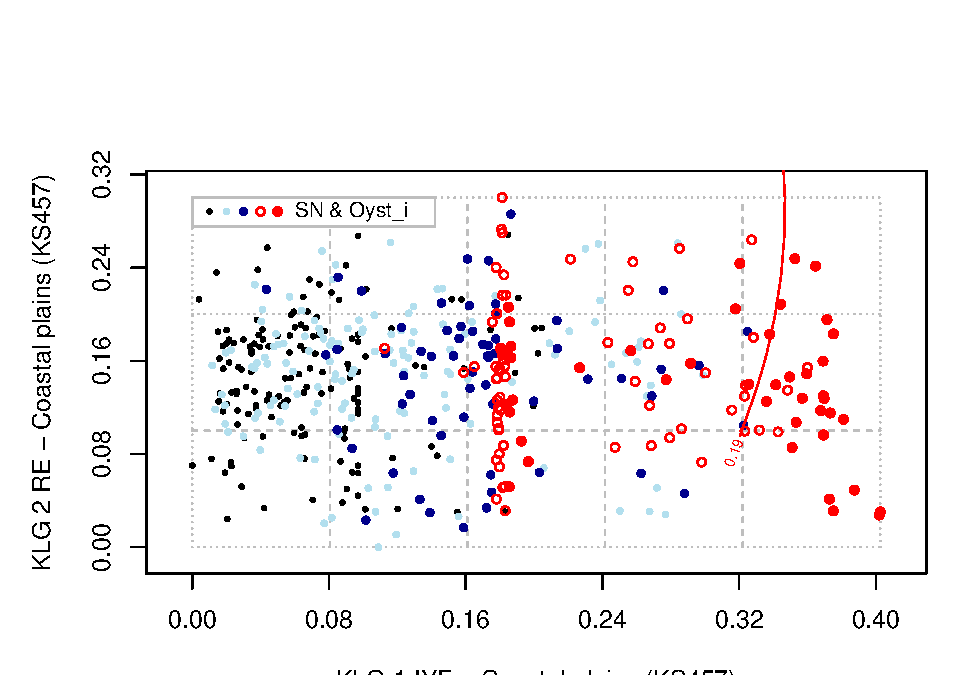
\includegraphics{Landscape_analysis_example_4_files/figure-latex/unnamed-chunk-42-1.pdf}

\begin{Shaded}
\begin{Highlighting}[]
  \CommentTok{#Plotter OI-klasser p? figuren, og legger p? isolinjer for IfIu}
  \KeywordTok{par}\NormalTok{(}\DataTypeTok{plt=}\KeywordTok{c}\NormalTok{(}\FloatTok{0.15}\NormalTok{, }\FloatTok{0.95}\NormalTok{, }\FloatTok{0.15}\NormalTok{, y2))}
\KeywordTok{plot}\NormalTok{(s1,s2,}\DataTypeTok{xlab=}\StringTok{"KLG 1 IYF - Coastal plains (KS457)"}\NormalTok{,}\DataTypeTok{ylab=}\StringTok{"KLG 2 RE - Coastal plains (KS457)"}\NormalTok{,}\DataTypeTok{xlim=}\KeywordTok{c}\NormalTok{(}\OperatorTok{-}\FloatTok{0.01}\NormalTok{,}\KeywordTok{max}\NormalTok{(s1)}\OperatorTok{+}\FloatTok{0.01}\NormalTok{),}\DataTypeTok{ylim=}\KeywordTok{c}\NormalTok{(}\OperatorTok{-}\FloatTok{0.01}\NormalTok{,}\KeywordTok{max}\NormalTok{(s2)}\OperatorTok{+}\FloatTok{0.01}\NormalTok{),}\DataTypeTok{xaxp=}\KeywordTok{c}\NormalTok{(}\DecValTok{0}\NormalTok{,}\FloatTok{0.4}\NormalTok{,}\DecValTok{5}\NormalTok{),}\DataTypeTok{yaxp=}\KeywordTok{c}\NormalTok{(}\DecValTok{0}\NormalTok{,}\FloatTok{0.4}\NormalTok{,}\DecValTok{5}\NormalTok{),}\DataTypeTok{type=}\StringTok{"n"}\NormalTok{) }\CommentTok{#Grunnlag for plotting av symboler etc.}
\KeywordTok{lines}\NormalTok{(}\KeywordTok{c}\NormalTok{(}\DecValTok{0}\NormalTok{,}\KeywordTok{max}\NormalTok{(s1)),}\KeywordTok{c}\NormalTok{(}\KeywordTok{max}\NormalTok{(s2),}\KeywordTok{max}\NormalTok{(s2)),}\DataTypeTok{lty=}\DecValTok{3}\NormalTok{,}\DataTypeTok{col=}\DecValTok{8}\NormalTok{)}
\KeywordTok{lines}\NormalTok{(}\KeywordTok{c}\NormalTok{(}\DecValTok{0}\NormalTok{,}\KeywordTok{max}\NormalTok{(s1)),}\KeywordTok{c}\NormalTok{(}\DecValTok{0}\NormalTok{,}\DecValTok{0}\NormalTok{),}\DataTypeTok{lty=}\DecValTok{3}\NormalTok{,}\DataTypeTok{col=}\DecValTok{8}\NormalTok{)}
\KeywordTok{lines}\NormalTok{(}\KeywordTok{c}\NormalTok{(}\DecValTok{0}\NormalTok{,}\DecValTok{0}\NormalTok{),}\KeywordTok{c}\NormalTok{(}\DecValTok{0}\NormalTok{,}\KeywordTok{max}\NormalTok{(s2)),}\DataTypeTok{lty=}\DecValTok{3}\NormalTok{,}\DataTypeTok{col=}\DecValTok{8}\NormalTok{)}
\KeywordTok{lines}\NormalTok{(}\KeywordTok{c}\NormalTok{(}\KeywordTok{max}\NormalTok{(s1),}\KeywordTok{max}\NormalTok{(s1)),}\KeywordTok{c}\NormalTok{(}\DecValTok{0}\NormalTok{,}\KeywordTok{max}\NormalTok{(s2)),}\DataTypeTok{lty=}\DecValTok{3}\NormalTok{,}\DataTypeTok{col=}\DecValTok{8}\NormalTok{)}

\KeywordTok{lines}\NormalTok{(}\KeywordTok{c}\NormalTok{(}\DecValTok{0}\NormalTok{,}\KeywordTok{max}\NormalTok{(s1)),}\KeywordTok{c}\NormalTok{(}\KeywordTok{max}\NormalTok{(s2)}\OperatorTok{/}\DecValTok{3}\NormalTok{,}\KeywordTok{max}\NormalTok{(s2)}\OperatorTok{/}\DecValTok{3}\NormalTok{),}\DataTypeTok{lty=}\DecValTok{2}\NormalTok{,}\DataTypeTok{col=}\DecValTok{8}\NormalTok{)}
\KeywordTok{lines}\NormalTok{(}\KeywordTok{c}\NormalTok{(}\DecValTok{0}\NormalTok{,}\KeywordTok{max}\NormalTok{(s1)),}\KeywordTok{c}\NormalTok{(}\DecValTok{2}\OperatorTok{*}\KeywordTok{max}\NormalTok{(s2)}\OperatorTok{/}\DecValTok{3}\NormalTok{,}\DecValTok{2}\OperatorTok{*}\KeywordTok{max}\NormalTok{(s2)}\OperatorTok{/}\DecValTok{3}\NormalTok{),}\DataTypeTok{lty=}\DecValTok{3}\NormalTok{,}\DataTypeTok{col=}\DecValTok{8}\NormalTok{)}
\KeywordTok{lines}\NormalTok{(}\KeywordTok{c}\NormalTok{(}\FloatTok{0.2}\OperatorTok{*}\KeywordTok{max}\NormalTok{(s1),}\FloatTok{0.2}\OperatorTok{*}\KeywordTok{max}\NormalTok{(s1)),}\KeywordTok{c}\NormalTok{(}\DecValTok{0}\NormalTok{,}\KeywordTok{max}\NormalTok{(s2)}\OperatorTok{-}\FloatTok{0.025}\NormalTok{),}\DataTypeTok{lty=}\DecValTok{2}\NormalTok{,}\DataTypeTok{col=}\DecValTok{8}\NormalTok{)}
\KeywordTok{lines}\NormalTok{(}\KeywordTok{c}\NormalTok{(}\FloatTok{0.4}\OperatorTok{*}\KeywordTok{max}\NormalTok{(s1),}\FloatTok{0.4}\OperatorTok{*}\KeywordTok{max}\NormalTok{(s1)),}\KeywordTok{c}\NormalTok{(}\DecValTok{0}\NormalTok{,}\KeywordTok{max}\NormalTok{(s2)),}\DataTypeTok{lty=}\DecValTok{2}\NormalTok{,}\DataTypeTok{col=}\DecValTok{8}\NormalTok{)}
\KeywordTok{lines}\NormalTok{(}\KeywordTok{c}\NormalTok{(}\FloatTok{0.6}\OperatorTok{*}\KeywordTok{max}\NormalTok{(s1),}\FloatTok{0.6}\OperatorTok{*}\KeywordTok{max}\NormalTok{(s1)),}\KeywordTok{c}\NormalTok{(}\DecValTok{0}\NormalTok{,}\KeywordTok{max}\NormalTok{(s2)),}\DataTypeTok{lty=}\DecValTok{2}\NormalTok{,}\DataTypeTok{col=}\DecValTok{8}\NormalTok{)}
\KeywordTok{lines}\NormalTok{(}\KeywordTok{c}\NormalTok{(}\FloatTok{0.8}\OperatorTok{*}\KeywordTok{max}\NormalTok{(s1),}\FloatTok{0.8}\OperatorTok{*}\KeywordTok{max}\NormalTok{(s1)),}\KeywordTok{c}\NormalTok{(}\DecValTok{0}\NormalTok{,}\KeywordTok{max}\NormalTok{(s2)),}\DataTypeTok{lty=}\DecValTok{2}\NormalTok{,}\DataTypeTok{col=}\DecValTok{8}\NormalTok{)}

\KeywordTok{lines}\NormalTok{(}\KeywordTok{c}\NormalTok{(}\DecValTok{0}\NormalTok{,}\FloatTok{0.142}\NormalTok{),}\KeywordTok{c}\NormalTok{(}\KeywordTok{max}\NormalTok{(s2),}\KeywordTok{max}\NormalTok{(s2)),}\DataTypeTok{col=}\DecValTok{8}\NormalTok{)}
\KeywordTok{lines}\NormalTok{(}\KeywordTok{c}\NormalTok{(}\DecValTok{0}\NormalTok{,}\FloatTok{0.142}\NormalTok{),}\KeywordTok{c}\NormalTok{(}\KeywordTok{max}\NormalTok{(s2)}\OperatorTok{-}\FloatTok{0.025}\NormalTok{,}\KeywordTok{max}\NormalTok{(s2)}\OperatorTok{-}\FloatTok{0.025}\NormalTok{),}\DataTypeTok{col=}\DecValTok{8}\NormalTok{)}
\KeywordTok{lines}\NormalTok{(}\KeywordTok{c}\NormalTok{(}\FloatTok{0.142}\NormalTok{,}\FloatTok{0.142}\NormalTok{),}\KeywordTok{c}\NormalTok{(}\KeywordTok{max}\NormalTok{(s2)}\OperatorTok{-}\FloatTok{0.025}\NormalTok{,}\KeywordTok{max}\NormalTok{(s2)),}\DataTypeTok{col=}\DecValTok{8}\NormalTok{)}
\KeywordTok{lines}\NormalTok{(}\KeywordTok{c}\NormalTok{(}\DecValTok{0}\NormalTok{,}\DecValTok{0}\NormalTok{),}\KeywordTok{c}\NormalTok{(}\KeywordTok{max}\NormalTok{(s2)}\OperatorTok{-}\FloatTok{0.025}\NormalTok{,}\KeywordTok{max}\NormalTok{(s2)),}\DataTypeTok{col=}\DecValTok{8}\NormalTok{)}
\KeywordTok{points}\NormalTok{(}\FloatTok{0.01}\NormalTok{,}\KeywordTok{max}\NormalTok{(s2)}\OperatorTok{-}\FloatTok{0.012}\NormalTok{,}\DataTypeTok{pch=}\DecValTok{1}\NormalTok{,}\DataTypeTok{cex=}\FloatTok{0.6}\NormalTok{,}\DataTypeTok{col=}\StringTok{"lightblue3"}\NormalTok{)}
\KeywordTok{points}\NormalTok{(}\FloatTok{0.02}\NormalTok{,}\KeywordTok{max}\NormalTok{(s2)}\OperatorTok{-}\FloatTok{0.012}\NormalTok{,}\DataTypeTok{pch=}\DecValTok{16}\NormalTok{,}\DataTypeTok{cex=}\FloatTok{0.6}\NormalTok{,}\DataTypeTok{col=}\StringTok{"lightblue3"}\NormalTok{)}
\KeywordTok{points}\NormalTok{(}\FloatTok{0.03}\NormalTok{,}\KeywordTok{max}\NormalTok{(s2)}\OperatorTok{-}\FloatTok{0.012}\NormalTok{,}\DataTypeTok{pch=}\DecValTok{1}\NormalTok{,}\DataTypeTok{cex=}\FloatTok{0.75}\NormalTok{,}\DataTypeTok{col=}\StringTok{"lightblue4"}\NormalTok{)}
\KeywordTok{points}\NormalTok{(}\FloatTok{0.04}\NormalTok{,}\KeywordTok{max}\NormalTok{(s2)}\OperatorTok{-}\FloatTok{0.012}\NormalTok{,}\DataTypeTok{pch=}\DecValTok{16}\NormalTok{,}\DataTypeTok{cex=}\FloatTok{0.75}\NormalTok{,}\DataTypeTok{col=}\StringTok{"lightblue4"}\NormalTok{)}
\KeywordTok{points}\NormalTok{(}\FloatTok{0.05}\NormalTok{,}\KeywordTok{max}\NormalTok{(s2)}\OperatorTok{-}\FloatTok{0.012}\NormalTok{,}\DataTypeTok{pch=}\DecValTok{1}\NormalTok{,}\DataTypeTok{cex=}\FloatTok{0.9}\NormalTok{,}\DataTypeTok{col=}\StringTok{"red"}\NormalTok{)}
\KeywordTok{points}\NormalTok{(}\FloatTok{0.06}\NormalTok{,}\KeywordTok{max}\NormalTok{(s2)}\OperatorTok{-}\FloatTok{0.012}\NormalTok{,}\DataTypeTok{pch=}\DecValTok{16}\NormalTok{,}\DataTypeTok{cex=}\FloatTok{0.9}\NormalTok{,}\DataTypeTok{col=}\StringTok{"red"}\NormalTok{)}

\KeywordTok{text}\NormalTok{(}\FloatTok{0.07}\NormalTok{,}\KeywordTok{max}\NormalTok{(s2)}\OperatorTok{-}\FloatTok{0.012}\NormalTok{,}\StringTok{"OI & IfIu"}\NormalTok{,}\DataTypeTok{adj=}\DecValTok{0}\NormalTok{,}\DataTypeTok{cex=}\FloatTok{0.8}\NormalTok{)}
\KeywordTok{points}\NormalTok{(s1[OI}\OperatorTok{==}\DecValTok{1}\NormalTok{],s2[OI}\OperatorTok{==}\DecValTok{1}\NormalTok{],}\DataTypeTok{pch=}\DecValTok{1}\NormalTok{,}\DataTypeTok{cex=}\FloatTok{0.6}\NormalTok{,}\DataTypeTok{col=}\StringTok{"lightblue3"}\NormalTok{)}
\KeywordTok{points}\NormalTok{(s1[OI}\OperatorTok{==}\DecValTok{2}\NormalTok{],s2[OI}\OperatorTok{==}\DecValTok{2}\NormalTok{],}\DataTypeTok{pch=}\DecValTok{16}\NormalTok{,}\DataTypeTok{cex=}\FloatTok{0.6}\NormalTok{,}\DataTypeTok{col=}\StringTok{"lightblue3"}\NormalTok{)}
\KeywordTok{points}\NormalTok{(s1[OI}\OperatorTok{==}\DecValTok{3}\NormalTok{],s2[OI}\OperatorTok{==}\DecValTok{3}\NormalTok{],}\DataTypeTok{pch=}\DecValTok{1}\NormalTok{,}\DataTypeTok{cex=}\FloatTok{0.75}\NormalTok{,}\DataTypeTok{col=}\StringTok{"lightblue4"}\NormalTok{)}
\KeywordTok{points}\NormalTok{(s1[OI}\OperatorTok{==}\DecValTok{4}\NormalTok{],s2[OI}\OperatorTok{==}\DecValTok{4}\NormalTok{],}\DataTypeTok{pch=}\DecValTok{16}\NormalTok{,}\DataTypeTok{cex=}\FloatTok{0.75}\NormalTok{,}\DataTypeTok{col=}\StringTok{"lightblue4"}\NormalTok{)}
\KeywordTok{points}\NormalTok{(s1[OI}\OperatorTok{==}\DecValTok{5}\NormalTok{],s2[OI}\OperatorTok{==}\DecValTok{5}\NormalTok{],}\DataTypeTok{pch=}\DecValTok{1}\NormalTok{,}\DataTypeTok{cex=}\FloatTok{0.9}\NormalTok{,}\DataTypeTok{col=}\StringTok{"red"}\NormalTok{)}
\KeywordTok{points}\NormalTok{(s1[OI}\OperatorTok{==}\DecValTok{6}\NormalTok{],s2[OI}\OperatorTok{==}\DecValTok{6}\NormalTok{],}\DataTypeTok{pch=}\DecValTok{16}\NormalTok{,}\DataTypeTok{cex=}\FloatTok{0.9}\NormalTok{,}\DataTypeTok{col=}\StringTok{"red"}\NormalTok{)}

\NormalTok{os <-}\StringTok{ }\KeywordTok{ordisurf}\NormalTok{(snv[,}\KeywordTok{c}\NormalTok{(}\DecValTok{1}\NormalTok{,}\DecValTok{2}\NormalTok{)],IfIu,}\DataTypeTok{display=}\StringTok{"sites"}\NormalTok{,}\DataTypeTok{levels=}\KeywordTok{c}\NormalTok{(}\DecValTok{1}\NormalTok{,}\DecValTok{2}\NormalTok{,}\DecValTok{4}\NormalTok{,}\DecValTok{6}\NormalTok{,}\DecValTok{8}\NormalTok{,}\DecValTok{10}\NormalTok{,}\DecValTok{11}\NormalTok{), }\DataTypeTok{col=}\StringTok{"red"}\NormalTok{,}\DataTypeTok{add=}\NormalTok{T) }\CommentTok{#inkluderer plotting p? eksisterende ordinasjonsdiagram}
\end{Highlighting}
\end{Shaded}

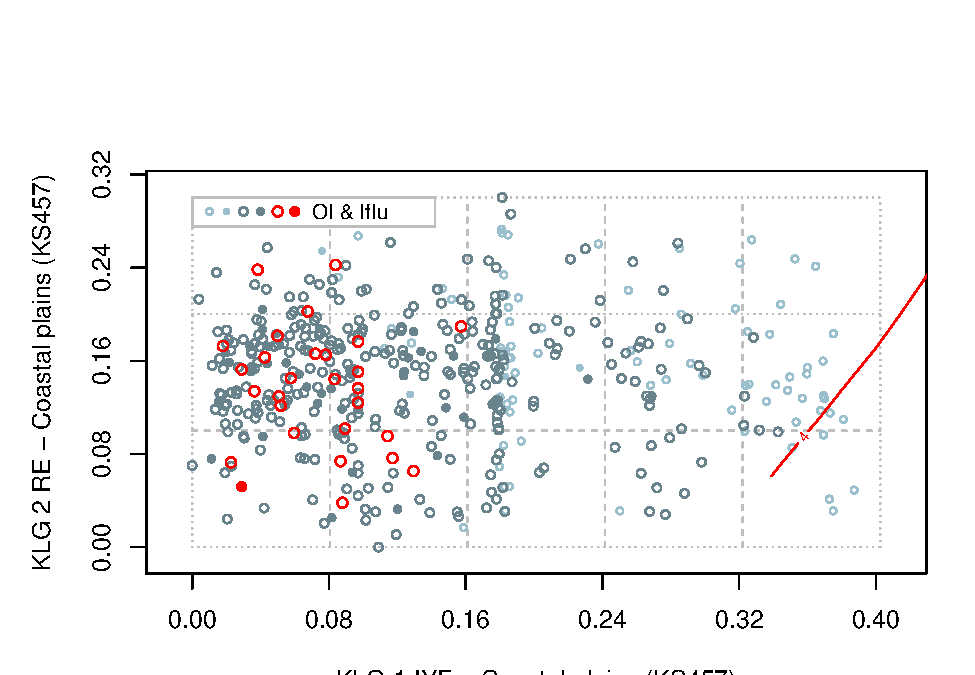
\includegraphics{Landscape_analysis_example_4_files/figure-latex/unnamed-chunk-43-1.pdf}

\begin{Shaded}
\begin{Highlighting}[]
\CommentTok{#Plotter JP-klasser p? figuren, og legger p? isolinjer for Ar_full}
  \KeywordTok{par}\NormalTok{(}\DataTypeTok{plt=}\KeywordTok{c}\NormalTok{(}\FloatTok{0.15}\NormalTok{, }\FloatTok{0.95}\NormalTok{, }\FloatTok{0.15}\NormalTok{, y2))}
\KeywordTok{plot}\NormalTok{(s1,s2,}\DataTypeTok{xlab=}\StringTok{"KLG 1 IYF - Coastal plains (KS457)"}\NormalTok{,}\DataTypeTok{ylab=}\StringTok{"KLG 2 RE - Coastal plains (KS457)"}\NormalTok{,}\DataTypeTok{xlim=}\KeywordTok{c}\NormalTok{(}\OperatorTok{-}\FloatTok{0.01}\NormalTok{,}\KeywordTok{max}\NormalTok{(s1)}\OperatorTok{+}\FloatTok{0.01}\NormalTok{),}\DataTypeTok{ylim=}\KeywordTok{c}\NormalTok{(}\OperatorTok{-}\FloatTok{0.01}\NormalTok{,}\KeywordTok{max}\NormalTok{(s2)}\OperatorTok{+}\FloatTok{0.01}\NormalTok{),}\DataTypeTok{xaxp=}\KeywordTok{c}\NormalTok{(}\DecValTok{0}\NormalTok{,}\FloatTok{0.4}\NormalTok{,}\DecValTok{5}\NormalTok{),}\DataTypeTok{yaxp=}\KeywordTok{c}\NormalTok{(}\DecValTok{0}\NormalTok{,}\FloatTok{0.4}\NormalTok{,}\DecValTok{5}\NormalTok{),}\DataTypeTok{type=}\StringTok{"n"}\NormalTok{) }\CommentTok{#Grunnlag for plotting av symboler etc.}
\KeywordTok{lines}\NormalTok{(}\KeywordTok{c}\NormalTok{(}\DecValTok{0}\NormalTok{,}\KeywordTok{max}\NormalTok{(s1)),}\KeywordTok{c}\NormalTok{(}\KeywordTok{max}\NormalTok{(s2),}\KeywordTok{max}\NormalTok{(s2)),}\DataTypeTok{lty=}\DecValTok{3}\NormalTok{,}\DataTypeTok{col=}\DecValTok{8}\NormalTok{)}
\KeywordTok{lines}\NormalTok{(}\KeywordTok{c}\NormalTok{(}\DecValTok{0}\NormalTok{,}\KeywordTok{max}\NormalTok{(s1)),}\KeywordTok{c}\NormalTok{(}\DecValTok{0}\NormalTok{,}\DecValTok{0}\NormalTok{),}\DataTypeTok{lty=}\DecValTok{3}\NormalTok{,}\DataTypeTok{col=}\DecValTok{8}\NormalTok{)}
\KeywordTok{lines}\NormalTok{(}\KeywordTok{c}\NormalTok{(}\DecValTok{0}\NormalTok{,}\DecValTok{0}\NormalTok{),}\KeywordTok{c}\NormalTok{(}\DecValTok{0}\NormalTok{,}\KeywordTok{max}\NormalTok{(s2)),}\DataTypeTok{lty=}\DecValTok{3}\NormalTok{,}\DataTypeTok{col=}\DecValTok{8}\NormalTok{)}
\KeywordTok{lines}\NormalTok{(}\KeywordTok{c}\NormalTok{(}\KeywordTok{max}\NormalTok{(s1),}\KeywordTok{max}\NormalTok{(s1)),}\KeywordTok{c}\NormalTok{(}\DecValTok{0}\NormalTok{,}\KeywordTok{max}\NormalTok{(s2)),}\DataTypeTok{lty=}\DecValTok{3}\NormalTok{,}\DataTypeTok{col=}\DecValTok{8}\NormalTok{)}

\KeywordTok{lines}\NormalTok{(}\KeywordTok{c}\NormalTok{(}\DecValTok{0}\NormalTok{,}\KeywordTok{max}\NormalTok{(s1)),}\KeywordTok{c}\NormalTok{(}\KeywordTok{max}\NormalTok{(s2)}\OperatorTok{/}\DecValTok{3}\NormalTok{,}\KeywordTok{max}\NormalTok{(s2)}\OperatorTok{/}\DecValTok{3}\NormalTok{),}\DataTypeTok{lty=}\DecValTok{2}\NormalTok{,}\DataTypeTok{col=}\DecValTok{8}\NormalTok{)}
\KeywordTok{lines}\NormalTok{(}\KeywordTok{c}\NormalTok{(}\DecValTok{0}\NormalTok{,}\KeywordTok{max}\NormalTok{(s1)),}\KeywordTok{c}\NormalTok{(}\DecValTok{2}\OperatorTok{*}\KeywordTok{max}\NormalTok{(s2)}\OperatorTok{/}\DecValTok{3}\NormalTok{,}\DecValTok{2}\OperatorTok{*}\KeywordTok{max}\NormalTok{(s2)}\OperatorTok{/}\DecValTok{3}\NormalTok{),}\DataTypeTok{lty=}\DecValTok{3}\NormalTok{,}\DataTypeTok{col=}\DecValTok{8}\NormalTok{)}
\KeywordTok{lines}\NormalTok{(}\KeywordTok{c}\NormalTok{(}\FloatTok{0.2}\OperatorTok{*}\KeywordTok{max}\NormalTok{(s1),}\FloatTok{0.2}\OperatorTok{*}\KeywordTok{max}\NormalTok{(s1)),}\KeywordTok{c}\NormalTok{(}\DecValTok{0}\NormalTok{,}\KeywordTok{max}\NormalTok{(s2)}\OperatorTok{-}\FloatTok{0.025}\NormalTok{),}\DataTypeTok{lty=}\DecValTok{2}\NormalTok{,}\DataTypeTok{col=}\DecValTok{8}\NormalTok{)}
\KeywordTok{lines}\NormalTok{(}\KeywordTok{c}\NormalTok{(}\FloatTok{0.4}\OperatorTok{*}\KeywordTok{max}\NormalTok{(s1),}\FloatTok{0.4}\OperatorTok{*}\KeywordTok{max}\NormalTok{(s1)),}\KeywordTok{c}\NormalTok{(}\DecValTok{0}\NormalTok{,}\KeywordTok{max}\NormalTok{(s2)),}\DataTypeTok{lty=}\DecValTok{2}\NormalTok{,}\DataTypeTok{col=}\DecValTok{8}\NormalTok{)}
\KeywordTok{lines}\NormalTok{(}\KeywordTok{c}\NormalTok{(}\FloatTok{0.6}\OperatorTok{*}\KeywordTok{max}\NormalTok{(s1),}\FloatTok{0.6}\OperatorTok{*}\KeywordTok{max}\NormalTok{(s1)),}\KeywordTok{c}\NormalTok{(}\DecValTok{0}\NormalTok{,}\KeywordTok{max}\NormalTok{(s2)),}\DataTypeTok{lty=}\DecValTok{2}\NormalTok{,}\DataTypeTok{col=}\DecValTok{8}\NormalTok{)}
\KeywordTok{lines}\NormalTok{(}\KeywordTok{c}\NormalTok{(}\FloatTok{0.8}\OperatorTok{*}\KeywordTok{max}\NormalTok{(s1),}\FloatTok{0.8}\OperatorTok{*}\KeywordTok{max}\NormalTok{(s1)),}\KeywordTok{c}\NormalTok{(}\DecValTok{0}\NormalTok{,}\KeywordTok{max}\NormalTok{(s2)),}\DataTypeTok{lty=}\DecValTok{2}\NormalTok{,}\DataTypeTok{col=}\DecValTok{8}\NormalTok{)}

\KeywordTok{lines}\NormalTok{(}\KeywordTok{c}\NormalTok{(}\DecValTok{0}\NormalTok{,}\FloatTok{0.142}\NormalTok{),}\KeywordTok{c}\NormalTok{(}\KeywordTok{max}\NormalTok{(s2),}\KeywordTok{max}\NormalTok{(s2)),}\DataTypeTok{col=}\DecValTok{8}\NormalTok{)}
\KeywordTok{lines}\NormalTok{(}\KeywordTok{c}\NormalTok{(}\DecValTok{0}\NormalTok{,}\FloatTok{0.142}\NormalTok{),}\KeywordTok{c}\NormalTok{(}\KeywordTok{max}\NormalTok{(s2)}\OperatorTok{-}\FloatTok{0.025}\NormalTok{,}\KeywordTok{max}\NormalTok{(s2)}\OperatorTok{-}\FloatTok{0.025}\NormalTok{),}\DataTypeTok{col=}\DecValTok{8}\NormalTok{)}
\KeywordTok{lines}\NormalTok{(}\KeywordTok{c}\NormalTok{(}\FloatTok{0.142}\NormalTok{,}\FloatTok{0.142}\NormalTok{),}\KeywordTok{c}\NormalTok{(}\KeywordTok{max}\NormalTok{(s2)}\OperatorTok{-}\FloatTok{0.025}\NormalTok{,}\KeywordTok{max}\NormalTok{(s2)),}\DataTypeTok{col=}\DecValTok{8}\NormalTok{)}
\KeywordTok{lines}\NormalTok{(}\KeywordTok{c}\NormalTok{(}\DecValTok{0}\NormalTok{,}\DecValTok{0}\NormalTok{),}\KeywordTok{c}\NormalTok{(}\KeywordTok{max}\NormalTok{(s2)}\OperatorTok{-}\FloatTok{0.025}\NormalTok{,}\KeywordTok{max}\NormalTok{(s2)),}\DataTypeTok{col=}\DecValTok{8}\NormalTok{)}
\KeywordTok{points}\NormalTok{(}\FloatTok{0.01}\NormalTok{,}\KeywordTok{max}\NormalTok{(s2)}\OperatorTok{-}\FloatTok{0.012}\NormalTok{,}\DataTypeTok{pch=}\DecValTok{1}\NormalTok{,}\DataTypeTok{cex=}\FloatTok{0.6}\NormalTok{,}\DataTypeTok{col=}\StringTok{"lightblue2"}\NormalTok{)}
\KeywordTok{points}\NormalTok{(}\FloatTok{0.02}\NormalTok{,}\KeywordTok{max}\NormalTok{(s2)}\OperatorTok{-}\FloatTok{0.012}\NormalTok{,}\DataTypeTok{pch=}\DecValTok{16}\NormalTok{,}\DataTypeTok{cex=}\FloatTok{0.75}\NormalTok{,}\DataTypeTok{col=}\StringTok{"lightblue4"}\NormalTok{)}
\KeywordTok{points}\NormalTok{(}\FloatTok{0.03}\NormalTok{,}\KeywordTok{max}\NormalTok{(s2)}\OperatorTok{-}\FloatTok{0.012}\NormalTok{,}\DataTypeTok{pch=}\DecValTok{16}\NormalTok{,}\DataTypeTok{cex=}\FloatTok{0.9}\NormalTok{,}\DataTypeTok{col=}\StringTok{"red"}\NormalTok{)}

\KeywordTok{text}\NormalTok{(}\FloatTok{0.04}\NormalTok{,}\KeywordTok{max}\NormalTok{(s2)}\OperatorTok{-}\FloatTok{0.012}\NormalTok{,}\StringTok{"JI & Arfull_a"}\NormalTok{,}\DataTypeTok{adj=}\DecValTok{0}\NormalTok{,}\DataTypeTok{cex=}\FloatTok{0.8}\NormalTok{)}

\KeywordTok{points}\NormalTok{(s1[JP}\OperatorTok{==}\DecValTok{1}\NormalTok{],s2[JP}\OperatorTok{==}\DecValTok{1}\NormalTok{],}\DataTypeTok{pch=}\DecValTok{1}\NormalTok{,}\DataTypeTok{cex=}\FloatTok{0.6}\NormalTok{,}\DataTypeTok{col=}\StringTok{"lightblue2"}\NormalTok{)}
\KeywordTok{points}\NormalTok{(s1[JP}\OperatorTok{==}\DecValTok{2}\NormalTok{],s2[JP}\OperatorTok{==}\DecValTok{2}\NormalTok{],}\DataTypeTok{pch=}\DecValTok{16}\NormalTok{,}\DataTypeTok{cex=}\FloatTok{0.75}\NormalTok{,}\DataTypeTok{col=}\StringTok{"lightblue4"}\NormalTok{)}
\KeywordTok{points}\NormalTok{(s1[JP}\OperatorTok{==}\DecValTok{3}\NormalTok{],s2[JP}\OperatorTok{==}\DecValTok{3}\NormalTok{],}\DataTypeTok{pch=}\DecValTok{16}\NormalTok{,}\DataTypeTok{cex=}\FloatTok{0.9}\NormalTok{,}\DataTypeTok{col=}\StringTok{"red"}\NormalTok{)}

\NormalTok{os <-}\StringTok{ }\KeywordTok{ordisurf}\NormalTok{(snv[,}\KeywordTok{c}\NormalTok{(}\DecValTok{1}\NormalTok{,}\DecValTok{2}\NormalTok{)],Arfull_a,}\DataTypeTok{display=}\StringTok{"sites"}\NormalTok{,}\DataTypeTok{levels=}\KeywordTok{c}\NormalTok{(}\FloatTok{0.1}\NormalTok{,}\FloatTok{0.4}\NormalTok{,}\FloatTok{0.6}\NormalTok{), }\DataTypeTok{col=}\StringTok{"red"}\NormalTok{,}\DataTypeTok{add=}\NormalTok{T) }\CommentTok{#inkluderer plotting p? eksisterende ordinasjonsdiagram}
\end{Highlighting}
\end{Shaded}

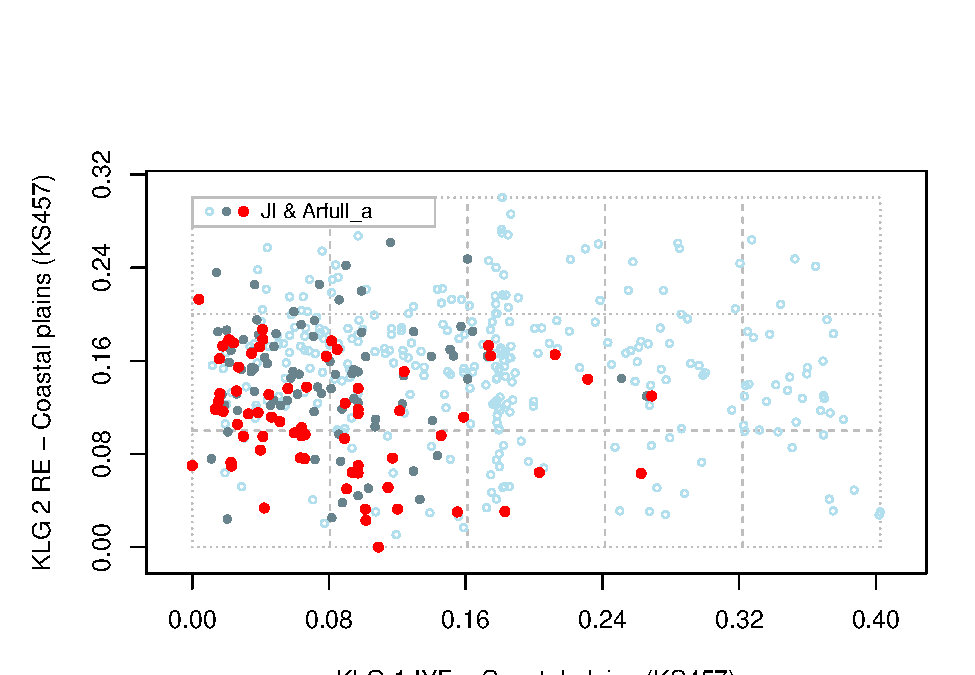
\includegraphics{Landscape_analysis_example_4_files/figure-latex/unnamed-chunk-44-1.pdf}

\begin{Shaded}
\begin{Highlighting}[]
\CommentTok{#Plotter MI-klasser p? figuren, og legger p? isolinjer for Mire_a}
  \KeywordTok{par}\NormalTok{(}\DataTypeTok{plt=}\KeywordTok{c}\NormalTok{(}\FloatTok{0.15}\NormalTok{, }\FloatTok{0.95}\NormalTok{, }\FloatTok{0.15}\NormalTok{, y2))}
\KeywordTok{plot}\NormalTok{(s1,s2,}\DataTypeTok{xlab=}\StringTok{"KLG 1 IYF - Coastal plains (KS457)"}\NormalTok{,}\DataTypeTok{ylab=}\StringTok{"KLG 2 RE - Coastal plains (KS457)"}\NormalTok{,}\DataTypeTok{xlim=}\KeywordTok{c}\NormalTok{(}\OperatorTok{-}\FloatTok{0.01}\NormalTok{,}\KeywordTok{max}\NormalTok{(s1)}\OperatorTok{+}\FloatTok{0.01}\NormalTok{),}\DataTypeTok{ylim=}\KeywordTok{c}\NormalTok{(}\OperatorTok{-}\FloatTok{0.01}\NormalTok{,}\KeywordTok{max}\NormalTok{(s2)}\OperatorTok{+}\FloatTok{0.01}\NormalTok{),}\DataTypeTok{xaxp=}\KeywordTok{c}\NormalTok{(}\DecValTok{0}\NormalTok{,}\FloatTok{0.4}\NormalTok{,}\DecValTok{5}\NormalTok{),}\DataTypeTok{yaxp=}\KeywordTok{c}\NormalTok{(}\DecValTok{0}\NormalTok{,}\FloatTok{0.4}\NormalTok{,}\DecValTok{5}\NormalTok{),}\DataTypeTok{type=}\StringTok{"n"}\NormalTok{) }\CommentTok{#Grunnlag for plotting av symboler etc.}
\KeywordTok{lines}\NormalTok{(}\KeywordTok{c}\NormalTok{(}\DecValTok{0}\NormalTok{,}\KeywordTok{max}\NormalTok{(s1)),}\KeywordTok{c}\NormalTok{(}\KeywordTok{max}\NormalTok{(s2),}\KeywordTok{max}\NormalTok{(s2)),}\DataTypeTok{lty=}\DecValTok{3}\NormalTok{,}\DataTypeTok{col=}\DecValTok{8}\NormalTok{)}
\KeywordTok{lines}\NormalTok{(}\KeywordTok{c}\NormalTok{(}\DecValTok{0}\NormalTok{,}\KeywordTok{max}\NormalTok{(s1)),}\KeywordTok{c}\NormalTok{(}\DecValTok{0}\NormalTok{,}\DecValTok{0}\NormalTok{),}\DataTypeTok{lty=}\DecValTok{3}\NormalTok{,}\DataTypeTok{col=}\DecValTok{8}\NormalTok{)}
\KeywordTok{lines}\NormalTok{(}\KeywordTok{c}\NormalTok{(}\DecValTok{0}\NormalTok{,}\DecValTok{0}\NormalTok{),}\KeywordTok{c}\NormalTok{(}\DecValTok{0}\NormalTok{,}\KeywordTok{max}\NormalTok{(s2)),}\DataTypeTok{lty=}\DecValTok{3}\NormalTok{,}\DataTypeTok{col=}\DecValTok{8}\NormalTok{)}
\KeywordTok{lines}\NormalTok{(}\KeywordTok{c}\NormalTok{(}\KeywordTok{max}\NormalTok{(s1),}\KeywordTok{max}\NormalTok{(s1)),}\KeywordTok{c}\NormalTok{(}\DecValTok{0}\NormalTok{,}\KeywordTok{max}\NormalTok{(s2)),}\DataTypeTok{lty=}\DecValTok{3}\NormalTok{,}\DataTypeTok{col=}\DecValTok{8}\NormalTok{)}

\KeywordTok{lines}\NormalTok{(}\KeywordTok{c}\NormalTok{(}\DecValTok{0}\NormalTok{,}\KeywordTok{max}\NormalTok{(s1)),}\KeywordTok{c}\NormalTok{(}\KeywordTok{max}\NormalTok{(s2)}\OperatorTok{/}\DecValTok{3}\NormalTok{,}\KeywordTok{max}\NormalTok{(s2)}\OperatorTok{/}\DecValTok{3}\NormalTok{),}\DataTypeTok{lty=}\DecValTok{2}\NormalTok{,}\DataTypeTok{col=}\DecValTok{8}\NormalTok{)}
\KeywordTok{lines}\NormalTok{(}\KeywordTok{c}\NormalTok{(}\DecValTok{0}\NormalTok{,}\KeywordTok{max}\NormalTok{(s1)),}\KeywordTok{c}\NormalTok{(}\DecValTok{2}\OperatorTok{*}\KeywordTok{max}\NormalTok{(s2)}\OperatorTok{/}\DecValTok{3}\NormalTok{,}\DecValTok{2}\OperatorTok{*}\KeywordTok{max}\NormalTok{(s2)}\OperatorTok{/}\DecValTok{3}\NormalTok{),}\DataTypeTok{lty=}\DecValTok{3}\NormalTok{,}\DataTypeTok{col=}\DecValTok{8}\NormalTok{)}
\KeywordTok{lines}\NormalTok{(}\KeywordTok{c}\NormalTok{(}\FloatTok{0.2}\OperatorTok{*}\KeywordTok{max}\NormalTok{(s1),}\FloatTok{0.2}\OperatorTok{*}\KeywordTok{max}\NormalTok{(s1)),}\KeywordTok{c}\NormalTok{(}\DecValTok{0}\NormalTok{,}\KeywordTok{max}\NormalTok{(s2)}\OperatorTok{-}\FloatTok{0.025}\NormalTok{),}\DataTypeTok{lty=}\DecValTok{2}\NormalTok{,}\DataTypeTok{col=}\DecValTok{8}\NormalTok{)}
\KeywordTok{lines}\NormalTok{(}\KeywordTok{c}\NormalTok{(}\FloatTok{0.4}\OperatorTok{*}\KeywordTok{max}\NormalTok{(s1),}\FloatTok{0.4}\OperatorTok{*}\KeywordTok{max}\NormalTok{(s1)),}\KeywordTok{c}\NormalTok{(}\DecValTok{0}\NormalTok{,}\KeywordTok{max}\NormalTok{(s2)),}\DataTypeTok{lty=}\DecValTok{2}\NormalTok{,}\DataTypeTok{col=}\DecValTok{8}\NormalTok{)}
\KeywordTok{lines}\NormalTok{(}\KeywordTok{c}\NormalTok{(}\FloatTok{0.6}\OperatorTok{*}\KeywordTok{max}\NormalTok{(s1),}\FloatTok{0.6}\OperatorTok{*}\KeywordTok{max}\NormalTok{(s1)),}\KeywordTok{c}\NormalTok{(}\DecValTok{0}\NormalTok{,}\KeywordTok{max}\NormalTok{(s2)),}\DataTypeTok{lty=}\DecValTok{2}\NormalTok{,}\DataTypeTok{col=}\DecValTok{8}\NormalTok{)}
\KeywordTok{lines}\NormalTok{(}\KeywordTok{c}\NormalTok{(}\FloatTok{0.8}\OperatorTok{*}\KeywordTok{max}\NormalTok{(s1),}\FloatTok{0.8}\OperatorTok{*}\KeywordTok{max}\NormalTok{(s1)),}\KeywordTok{c}\NormalTok{(}\DecValTok{0}\NormalTok{,}\KeywordTok{max}\NormalTok{(s2)),}\DataTypeTok{lty=}\DecValTok{2}\NormalTok{,}\DataTypeTok{col=}\DecValTok{8}\NormalTok{)}

\KeywordTok{lines}\NormalTok{(}\KeywordTok{c}\NormalTok{(}\DecValTok{0}\NormalTok{,}\FloatTok{0.142}\NormalTok{),}\KeywordTok{c}\NormalTok{(}\KeywordTok{max}\NormalTok{(s2),}\KeywordTok{max}\NormalTok{(s2)),}\DataTypeTok{col=}\DecValTok{8}\NormalTok{)}
\KeywordTok{lines}\NormalTok{(}\KeywordTok{c}\NormalTok{(}\DecValTok{0}\NormalTok{,}\FloatTok{0.142}\NormalTok{),}\KeywordTok{c}\NormalTok{(}\KeywordTok{max}\NormalTok{(s2)}\OperatorTok{-}\FloatTok{0.025}\NormalTok{,}\KeywordTok{max}\NormalTok{(s2)}\OperatorTok{-}\FloatTok{0.025}\NormalTok{),}\DataTypeTok{col=}\DecValTok{8}\NormalTok{)}
\KeywordTok{lines}\NormalTok{(}\KeywordTok{c}\NormalTok{(}\FloatTok{0.142}\NormalTok{,}\FloatTok{0.142}\NormalTok{),}\KeywordTok{c}\NormalTok{(}\KeywordTok{max}\NormalTok{(s2)}\OperatorTok{-}\FloatTok{0.025}\NormalTok{,}\KeywordTok{max}\NormalTok{(s2)),}\DataTypeTok{col=}\DecValTok{8}\NormalTok{)}
\KeywordTok{lines}\NormalTok{(}\KeywordTok{c}\NormalTok{(}\DecValTok{0}\NormalTok{,}\DecValTok{0}\NormalTok{),}\KeywordTok{c}\NormalTok{(}\KeywordTok{max}\NormalTok{(s2)}\OperatorTok{-}\FloatTok{0.025}\NormalTok{,}\KeywordTok{max}\NormalTok{(s2)),}\DataTypeTok{col=}\DecValTok{8}\NormalTok{)}
\KeywordTok{points}\NormalTok{(}\FloatTok{0.01}\NormalTok{,}\KeywordTok{max}\NormalTok{(s2)}\OperatorTok{-}\FloatTok{0.012}\NormalTok{,}\DataTypeTok{pch=}\DecValTok{1}\NormalTok{,}\DataTypeTok{cex=}\FloatTok{0.6}\NormalTok{,}\DataTypeTok{col=}\StringTok{"lightblue4"}\NormalTok{)}
\KeywordTok{points}\NormalTok{(}\FloatTok{0.02}\NormalTok{,}\KeywordTok{max}\NormalTok{(s2)}\OperatorTok{-}\FloatTok{0.012}\NormalTok{,}\DataTypeTok{pch=}\DecValTok{16}\NormalTok{,}\DataTypeTok{cex=}\FloatTok{0.6}\NormalTok{,}\DataTypeTok{col=}\StringTok{"red"}\NormalTok{)}

\KeywordTok{text}\NormalTok{(}\FloatTok{0.03}\NormalTok{,}\KeywordTok{max}\NormalTok{(s2)}\OperatorTok{-}\FloatTok{0.012}\NormalTok{,}\StringTok{"MP & Mire_a"}\NormalTok{,}\DataTypeTok{adj=}\DecValTok{0}\NormalTok{,}\DataTypeTok{cex=}\FloatTok{0.8}\NormalTok{)}

\KeywordTok{points}\NormalTok{(s1[MP}\OperatorTok{==}\DecValTok{1}\NormalTok{],s2[MP}\OperatorTok{==}\DecValTok{1}\NormalTok{],}\DataTypeTok{pch=}\DecValTok{16}\NormalTok{,}\DataTypeTok{cex=}\FloatTok{0.6}\NormalTok{,}\DataTypeTok{col=}\StringTok{"lightblue4"}\NormalTok{)}
\KeywordTok{points}\NormalTok{(s1[MP}\OperatorTok{==}\DecValTok{2}\NormalTok{],s2[MP}\OperatorTok{==}\DecValTok{2}\NormalTok{],}\DataTypeTok{pch=}\DecValTok{16}\NormalTok{,}\DataTypeTok{cex=}\FloatTok{0.6}\NormalTok{,}\DataTypeTok{col=}\StringTok{"red"}\NormalTok{)}

\NormalTok{os <-}\StringTok{ }\KeywordTok{ordisurf}\NormalTok{(snv[,}\KeywordTok{c}\NormalTok{(}\DecValTok{1}\NormalTok{,}\DecValTok{2}\NormalTok{)],Mire_a,}\DataTypeTok{display=}\StringTok{"sites"}\NormalTok{,}\DataTypeTok{levels=}\KeywordTok{c}\NormalTok{(}\FloatTok{0.05}\NormalTok{,}\FloatTok{0.1}\NormalTok{,}\FloatTok{0.2}\NormalTok{,}\FloatTok{0.4}\NormalTok{,}\FloatTok{0.6}\NormalTok{,}\FloatTok{0.8}\NormalTok{), }\DataTypeTok{col=}\StringTok{"red"}\NormalTok{,}\DataTypeTok{add=}\NormalTok{T) }\CommentTok{#inkluderer plotting p? eksisterende ordinasjonsdiagram}
\end{Highlighting}
\end{Shaded}

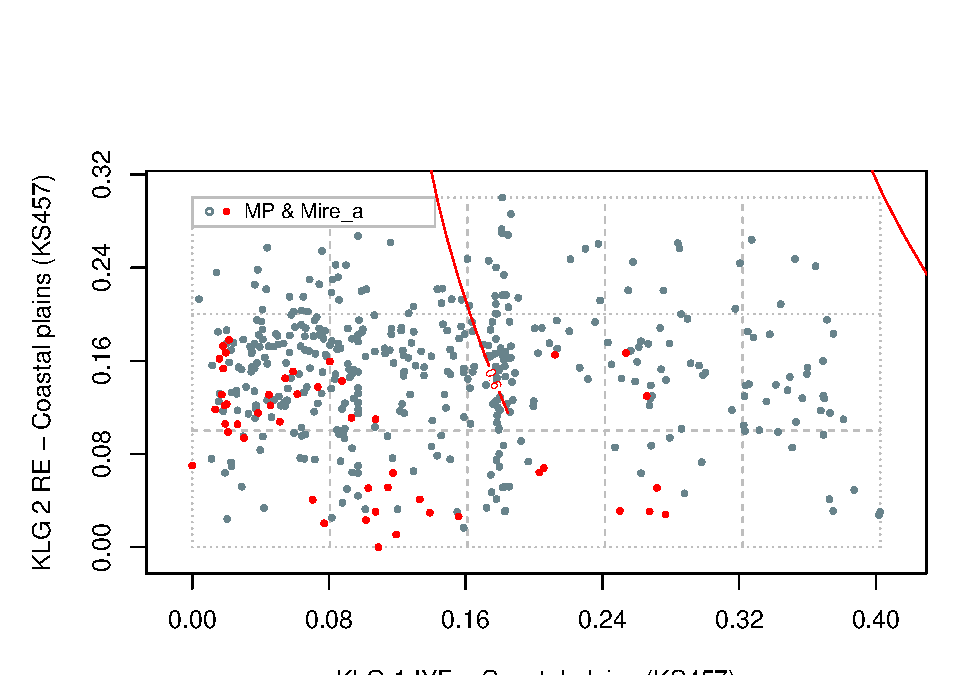
\includegraphics{Landscape_analysis_example_4_files/figure-latex/unnamed-chunk-45-1.pdf}

\begin{Shaded}
\begin{Highlighting}[]
\CommentTok{#Plotter RE-klasser p? figuren, og legger p? isolinjer for RR1}
\KeywordTok{par}\NormalTok{(}\DataTypeTok{plt=}\KeywordTok{c}\NormalTok{(}\FloatTok{0.15}\NormalTok{, }\FloatTok{0.95}\NormalTok{, }\FloatTok{0.15}\NormalTok{, y2))}
\KeywordTok{plot}\NormalTok{(s1,s2,}\DataTypeTok{xlab=}\StringTok{"KLG 1 IYF - Coastal plains (KS457)"}\NormalTok{,}\DataTypeTok{ylab=}\StringTok{"KLG 2 RE - Coastal plains (KS457)"}\NormalTok{,}\DataTypeTok{xlim=}\KeywordTok{c}\NormalTok{(}\OperatorTok{-}\FloatTok{0.01}\NormalTok{,}\KeywordTok{max}\NormalTok{(s1)}\OperatorTok{+}\FloatTok{0.01}\NormalTok{),}\DataTypeTok{ylim=}\KeywordTok{c}\NormalTok{(}\OperatorTok{-}\FloatTok{0.01}\NormalTok{,}\KeywordTok{max}\NormalTok{(s2)}\OperatorTok{+}\FloatTok{0.01}\NormalTok{),}\DataTypeTok{xaxp=}\KeywordTok{c}\NormalTok{(}\DecValTok{0}\NormalTok{,}\FloatTok{0.4}\NormalTok{,}\DecValTok{5}\NormalTok{),}\DataTypeTok{yaxp=}\KeywordTok{c}\NormalTok{(}\DecValTok{0}\NormalTok{,}\FloatTok{0.4}\NormalTok{,}\DecValTok{5}\NormalTok{),}\DataTypeTok{type=}\StringTok{"n"}\NormalTok{) }\CommentTok{#Grunnlag for plotting av symboler etc.}
\KeywordTok{lines}\NormalTok{(}\KeywordTok{c}\NormalTok{(}\DecValTok{0}\NormalTok{,}\KeywordTok{max}\NormalTok{(s1)),}\KeywordTok{c}\NormalTok{(}\KeywordTok{max}\NormalTok{(s2),}\KeywordTok{max}\NormalTok{(s2)),}\DataTypeTok{lty=}\DecValTok{3}\NormalTok{,}\DataTypeTok{col=}\DecValTok{8}\NormalTok{)}
\KeywordTok{lines}\NormalTok{(}\KeywordTok{c}\NormalTok{(}\DecValTok{0}\NormalTok{,}\KeywordTok{max}\NormalTok{(s1)),}\KeywordTok{c}\NormalTok{(}\DecValTok{0}\NormalTok{,}\DecValTok{0}\NormalTok{),}\DataTypeTok{lty=}\DecValTok{3}\NormalTok{,}\DataTypeTok{col=}\DecValTok{8}\NormalTok{)}
\KeywordTok{lines}\NormalTok{(}\KeywordTok{c}\NormalTok{(}\DecValTok{0}\NormalTok{,}\DecValTok{0}\NormalTok{),}\KeywordTok{c}\NormalTok{(}\DecValTok{0}\NormalTok{,}\KeywordTok{max}\NormalTok{(s2)),}\DataTypeTok{lty=}\DecValTok{3}\NormalTok{,}\DataTypeTok{col=}\DecValTok{8}\NormalTok{)}
\KeywordTok{lines}\NormalTok{(}\KeywordTok{c}\NormalTok{(}\KeywordTok{max}\NormalTok{(s1),}\KeywordTok{max}\NormalTok{(s1)),}\KeywordTok{c}\NormalTok{(}\DecValTok{0}\NormalTok{,}\KeywordTok{max}\NormalTok{(s2)),}\DataTypeTok{lty=}\DecValTok{3}\NormalTok{,}\DataTypeTok{col=}\DecValTok{8}\NormalTok{)}

\KeywordTok{lines}\NormalTok{(}\KeywordTok{c}\NormalTok{(}\DecValTok{0}\NormalTok{,}\KeywordTok{max}\NormalTok{(s1)),}\KeywordTok{c}\NormalTok{(}\KeywordTok{max}\NormalTok{(s2)}\OperatorTok{/}\DecValTok{3}\NormalTok{,}\KeywordTok{max}\NormalTok{(s2)}\OperatorTok{/}\DecValTok{3}\NormalTok{),}\DataTypeTok{lty=}\DecValTok{2}\NormalTok{,}\DataTypeTok{col=}\DecValTok{8}\NormalTok{)}
\KeywordTok{lines}\NormalTok{(}\KeywordTok{c}\NormalTok{(}\DecValTok{0}\NormalTok{,}\KeywordTok{max}\NormalTok{(s1)),}\KeywordTok{c}\NormalTok{(}\DecValTok{2}\OperatorTok{*}\KeywordTok{max}\NormalTok{(s2)}\OperatorTok{/}\DecValTok{3}\NormalTok{,}\DecValTok{2}\OperatorTok{*}\KeywordTok{max}\NormalTok{(s2)}\OperatorTok{/}\DecValTok{3}\NormalTok{),}\DataTypeTok{lty=}\DecValTok{3}\NormalTok{,}\DataTypeTok{col=}\DecValTok{8}\NormalTok{)}
\KeywordTok{lines}\NormalTok{(}\KeywordTok{c}\NormalTok{(}\FloatTok{0.2}\OperatorTok{*}\KeywordTok{max}\NormalTok{(s1),}\FloatTok{0.2}\OperatorTok{*}\KeywordTok{max}\NormalTok{(s1)),}\KeywordTok{c}\NormalTok{(}\DecValTok{0}\NormalTok{,}\KeywordTok{max}\NormalTok{(s2)}\OperatorTok{-}\FloatTok{0.025}\NormalTok{),}\DataTypeTok{lty=}\DecValTok{2}\NormalTok{,}\DataTypeTok{col=}\DecValTok{8}\NormalTok{)}
\KeywordTok{lines}\NormalTok{(}\KeywordTok{c}\NormalTok{(}\FloatTok{0.4}\OperatorTok{*}\KeywordTok{max}\NormalTok{(s1),}\FloatTok{0.4}\OperatorTok{*}\KeywordTok{max}\NormalTok{(s1)),}\KeywordTok{c}\NormalTok{(}\DecValTok{0}\NormalTok{,}\KeywordTok{max}\NormalTok{(s2)),}\DataTypeTok{lty=}\DecValTok{2}\NormalTok{,}\DataTypeTok{col=}\DecValTok{8}\NormalTok{)}
\KeywordTok{lines}\NormalTok{(}\KeywordTok{c}\NormalTok{(}\FloatTok{0.6}\OperatorTok{*}\KeywordTok{max}\NormalTok{(s1),}\FloatTok{0.6}\OperatorTok{*}\KeywordTok{max}\NormalTok{(s1)),}\KeywordTok{c}\NormalTok{(}\DecValTok{0}\NormalTok{,}\KeywordTok{max}\NormalTok{(s2)),}\DataTypeTok{lty=}\DecValTok{2}\NormalTok{,}\DataTypeTok{col=}\DecValTok{8}\NormalTok{)}
\KeywordTok{lines}\NormalTok{(}\KeywordTok{c}\NormalTok{(}\FloatTok{0.8}\OperatorTok{*}\KeywordTok{max}\NormalTok{(s1),}\FloatTok{0.8}\OperatorTok{*}\KeywordTok{max}\NormalTok{(s1)),}\KeywordTok{c}\NormalTok{(}\DecValTok{0}\NormalTok{,}\KeywordTok{max}\NormalTok{(s2)),}\DataTypeTok{lty=}\DecValTok{2}\NormalTok{,}\DataTypeTok{col=}\DecValTok{8}\NormalTok{)}

\KeywordTok{lines}\NormalTok{(}\KeywordTok{c}\NormalTok{(}\DecValTok{0}\NormalTok{,}\FloatTok{0.142}\NormalTok{),}\KeywordTok{c}\NormalTok{(}\KeywordTok{max}\NormalTok{(s2),}\KeywordTok{max}\NormalTok{(s2)),}\DataTypeTok{col=}\DecValTok{8}\NormalTok{)}
\KeywordTok{lines}\NormalTok{(}\KeywordTok{c}\NormalTok{(}\DecValTok{0}\NormalTok{,}\FloatTok{0.142}\NormalTok{),}\KeywordTok{c}\NormalTok{(}\KeywordTok{max}\NormalTok{(s2)}\OperatorTok{-}\FloatTok{0.025}\NormalTok{,}\KeywordTok{max}\NormalTok{(s2)}\OperatorTok{-}\FloatTok{0.025}\NormalTok{),}\DataTypeTok{col=}\DecValTok{8}\NormalTok{)}
\KeywordTok{lines}\NormalTok{(}\KeywordTok{c}\NormalTok{(}\FloatTok{0.142}\NormalTok{,}\FloatTok{0.142}\NormalTok{),}\KeywordTok{c}\NormalTok{(}\KeywordTok{max}\NormalTok{(s2)}\OperatorTok{-}\FloatTok{0.025}\NormalTok{,}\KeywordTok{max}\NormalTok{(s2)),}\DataTypeTok{col=}\DecValTok{8}\NormalTok{)}
\KeywordTok{lines}\NormalTok{(}\KeywordTok{c}\NormalTok{(}\DecValTok{0}\NormalTok{,}\DecValTok{0}\NormalTok{),}\KeywordTok{c}\NormalTok{(}\KeywordTok{max}\NormalTok{(s2)}\OperatorTok{-}\FloatTok{0.025}\NormalTok{,}\KeywordTok{max}\NormalTok{(s2)),}\DataTypeTok{col=}\DecValTok{8}\NormalTok{)}
\KeywordTok{points}\NormalTok{(}\FloatTok{0.01}\NormalTok{,}\KeywordTok{max}\NormalTok{(s2)}\OperatorTok{-}\FloatTok{0.012}\NormalTok{,}\DataTypeTok{pch=}\DecValTok{1}\NormalTok{,}\DataTypeTok{cex=}\FloatTok{0.6}\NormalTok{,}\DataTypeTok{col=}\StringTok{"lightblue4"}\NormalTok{)}
\KeywordTok{points}\NormalTok{(}\FloatTok{0.02}\NormalTok{,}\KeywordTok{max}\NormalTok{(s2)}\OperatorTok{-}\FloatTok{0.012}\NormalTok{,}\DataTypeTok{pch=}\DecValTok{16}\NormalTok{,}\DataTypeTok{cex=}\FloatTok{0.6}\NormalTok{,}\DataTypeTok{col=}\StringTok{"red"}\NormalTok{)}

\KeywordTok{points}\NormalTok{(}\FloatTok{0.01}\NormalTok{,}\KeywordTok{max}\NormalTok{(s2)}\OperatorTok{-}\FloatTok{0.012}\NormalTok{,}\DataTypeTok{pch=}\DecValTok{16}\NormalTok{,}\DataTypeTok{cex=}\FloatTok{0.5}\NormalTok{,}\DataTypeTok{col=}\StringTok{"black"}\NormalTok{)}
\KeywordTok{points}\NormalTok{(}\FloatTok{0.02}\NormalTok{,}\KeywordTok{max}\NormalTok{(s2)}\OperatorTok{-}\FloatTok{0.012}\NormalTok{,}\DataTypeTok{pch=}\DecValTok{16}\NormalTok{,}\DataTypeTok{cex=}\FloatTok{0.6}\NormalTok{,}\DataTypeTok{col=}\StringTok{"lightblue2"}\NormalTok{)}
\KeywordTok{points}\NormalTok{(}\FloatTok{0.03}\NormalTok{,}\KeywordTok{max}\NormalTok{(s2)}\OperatorTok{-}\FloatTok{0.012}\NormalTok{,}\DataTypeTok{pch=}\DecValTok{16}\NormalTok{,}\DataTypeTok{cex=}\FloatTok{0.75}\NormalTok{,}\DataTypeTok{col=}\StringTok{"darkblue"}\NormalTok{)}
\KeywordTok{points}\NormalTok{(}\FloatTok{0.04}\NormalTok{,}\KeywordTok{max}\NormalTok{(s2)}\OperatorTok{-}\FloatTok{0.012}\NormalTok{,}\DataTypeTok{pch=}\DecValTok{1}\NormalTok{,}\DataTypeTok{cex=}\FloatTok{0.75}\NormalTok{,}\DataTypeTok{col=}\StringTok{"red"}\NormalTok{)}
\KeywordTok{points}\NormalTok{(}\FloatTok{0.05}\NormalTok{,}\KeywordTok{max}\NormalTok{(s2)}\OperatorTok{-}\FloatTok{0.012}\NormalTok{,}\DataTypeTok{pch=}\DecValTok{16}\NormalTok{,}\DataTypeTok{cex=}\FloatTok{0.9}\NormalTok{,}\DataTypeTok{col=}\StringTok{"red"}\NormalTok{)}

\KeywordTok{text}\NormalTok{(}\FloatTok{0.06}\NormalTok{,}\KeywordTok{max}\NormalTok{(s2)}\OperatorTok{-}\FloatTok{0.012}\NormalTok{,}\StringTok{"SN & RR1"}\NormalTok{,}\DataTypeTok{adj=}\DecValTok{0}\NormalTok{,}\DataTypeTok{cex=}\FloatTok{0.8}\NormalTok{)}
\KeywordTok{points}\NormalTok{(s1[SN}\OperatorTok{==}\DecValTok{1}\NormalTok{],s2[SN}\OperatorTok{==}\DecValTok{1}\NormalTok{],}\DataTypeTok{pch=}\DecValTok{16}\NormalTok{,}\DataTypeTok{cex=}\FloatTok{0.5}\NormalTok{,}\DataTypeTok{col=}\DecValTok{1}\NormalTok{)}
\KeywordTok{points}\NormalTok{(s1[SN}\OperatorTok{==}\DecValTok{2}\NormalTok{],s2[SN}\OperatorTok{==}\DecValTok{2}\NormalTok{],}\DataTypeTok{pch=}\DecValTok{16}\NormalTok{,}\DataTypeTok{cex=}\FloatTok{0.6}\NormalTok{,}\DataTypeTok{col=}\StringTok{"lightblue2"}\NormalTok{)}
\KeywordTok{points}\NormalTok{(s1[SN}\OperatorTok{==}\DecValTok{3}\NormalTok{],s2[SN}\OperatorTok{==}\DecValTok{3}\NormalTok{],}\DataTypeTok{pch=}\DecValTok{16}\NormalTok{,}\DataTypeTok{cex=}\FloatTok{0.75}\NormalTok{,}\DataTypeTok{col=}\StringTok{"darkblue"}\NormalTok{)}
\KeywordTok{points}\NormalTok{(s1[SN}\OperatorTok{==}\DecValTok{4}\NormalTok{],s2[SN}\OperatorTok{==}\DecValTok{4}\NormalTok{],}\DataTypeTok{pch=}\DecValTok{1}\NormalTok{,}\DataTypeTok{cex=}\FloatTok{0.75}\NormalTok{,}\DataTypeTok{col=}\StringTok{"red"}\NormalTok{)}
\KeywordTok{points}\NormalTok{(s1[SN}\OperatorTok{==}\DecValTok{5}\NormalTok{],s2[SN}\OperatorTok{==}\DecValTok{5}\NormalTok{],}\DataTypeTok{pch=}\DecValTok{16}\NormalTok{,}\DataTypeTok{cex=}\FloatTok{0.9}\NormalTok{,}\DataTypeTok{col=}\StringTok{"red"}\NormalTok{)}

\NormalTok{os <-}\StringTok{ }\KeywordTok{ordisurf}\NormalTok{(snv[,}\KeywordTok{c}\NormalTok{(}\DecValTok{1}\NormalTok{,}\DecValTok{2}\NormalTok{)],RR1,}\DataTypeTok{display=}\StringTok{"sites"}\NormalTok{,}\DataTypeTok{levels=}\KeywordTok{c}\NormalTok{(}\DecValTok{25}\NormalTok{,}\DecValTok{50}\NormalTok{,}\DecValTok{75}\NormalTok{,}\DecValTok{100}\NormalTok{,}\DecValTok{150}\NormalTok{,}\DecValTok{200}\NormalTok{), }\DataTypeTok{col=}\StringTok{"red"}\NormalTok{,}\DataTypeTok{add=}\NormalTok{T) }\CommentTok{#inkluderer plotting p? eksisterende ordinasjonsdiagram}
\end{Highlighting}
\end{Shaded}

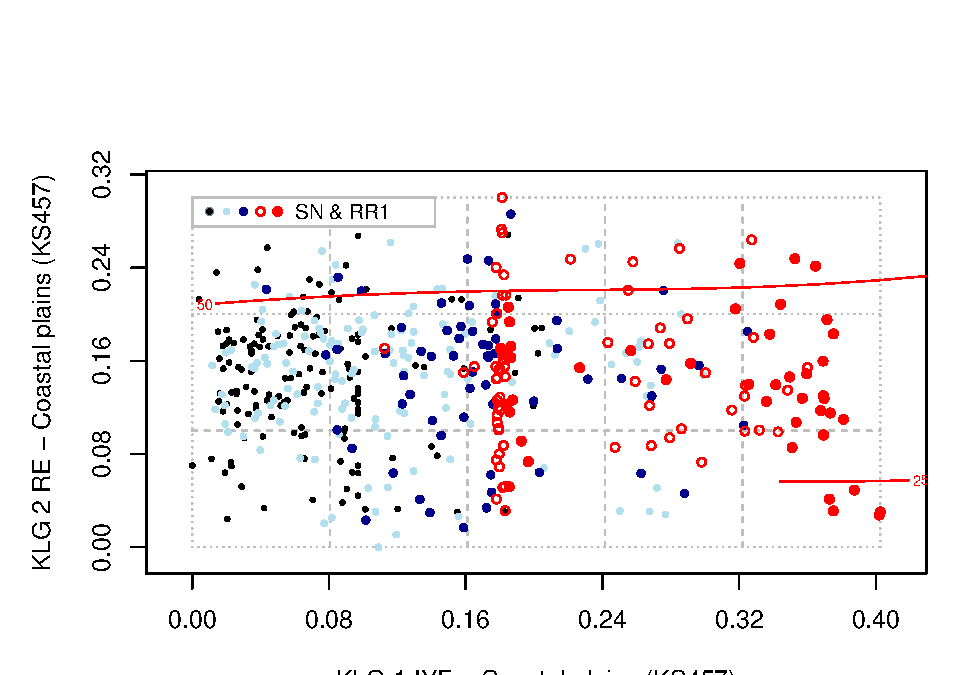
\includegraphics{Landscape_analysis_example_4_files/figure-latex/unnamed-chunk-46-1.pdf}

\begin{Shaded}
\begin{Highlighting}[]
\CommentTok{###}
\end{Highlighting}
\end{Shaded}

\begin{Shaded}
\begin{Highlighting}[]
\CommentTok{#Plotter RE-klasser p? figuren, og legger p? isolinjer for Rug3_m}
\KeywordTok{par}\NormalTok{(}\DataTypeTok{plt=}\KeywordTok{c}\NormalTok{(}\FloatTok{0.15}\NormalTok{, }\FloatTok{0.95}\NormalTok{, }\FloatTok{0.15}\NormalTok{, y2))}
\KeywordTok{plot}\NormalTok{(s1,s2,}\DataTypeTok{xlab=}\StringTok{"KLG 1 IYF - Coastal plains (KS457)"}\NormalTok{,}\DataTypeTok{ylab=}\StringTok{"KLG 2 RE - Coastal plains (KS457)"}\NormalTok{,}\DataTypeTok{xlim=}\KeywordTok{c}\NormalTok{(}\OperatorTok{-}\FloatTok{0.01}\NormalTok{,}\KeywordTok{max}\NormalTok{(s1)}\OperatorTok{+}\FloatTok{0.01}\NormalTok{),}\DataTypeTok{ylim=}\KeywordTok{c}\NormalTok{(}\OperatorTok{-}\FloatTok{0.01}\NormalTok{,}\KeywordTok{max}\NormalTok{(s2)}\OperatorTok{+}\FloatTok{0.01}\NormalTok{),}\DataTypeTok{xaxp=}\KeywordTok{c}\NormalTok{(}\DecValTok{0}\NormalTok{,}\FloatTok{0.4}\NormalTok{,}\DecValTok{5}\NormalTok{),}\DataTypeTok{yaxp=}\KeywordTok{c}\NormalTok{(}\DecValTok{0}\NormalTok{,}\FloatTok{0.4}\NormalTok{,}\DecValTok{5}\NormalTok{),}\DataTypeTok{type=}\StringTok{"n"}\NormalTok{) }\CommentTok{#Grunnlag for plotting av symboler etc.}
\KeywordTok{lines}\NormalTok{(}\KeywordTok{c}\NormalTok{(}\DecValTok{0}\NormalTok{,}\KeywordTok{max}\NormalTok{(s1)),}\KeywordTok{c}\NormalTok{(}\KeywordTok{max}\NormalTok{(s2),}\KeywordTok{max}\NormalTok{(s2)),}\DataTypeTok{lty=}\DecValTok{3}\NormalTok{,}\DataTypeTok{col=}\DecValTok{8}\NormalTok{)}
\KeywordTok{lines}\NormalTok{(}\KeywordTok{c}\NormalTok{(}\DecValTok{0}\NormalTok{,}\KeywordTok{max}\NormalTok{(s1)),}\KeywordTok{c}\NormalTok{(}\DecValTok{0}\NormalTok{,}\DecValTok{0}\NormalTok{),}\DataTypeTok{lty=}\DecValTok{3}\NormalTok{,}\DataTypeTok{col=}\DecValTok{8}\NormalTok{)}
\KeywordTok{lines}\NormalTok{(}\KeywordTok{c}\NormalTok{(}\DecValTok{0}\NormalTok{,}\DecValTok{0}\NormalTok{),}\KeywordTok{c}\NormalTok{(}\DecValTok{0}\NormalTok{,}\KeywordTok{max}\NormalTok{(s2)),}\DataTypeTok{lty=}\DecValTok{3}\NormalTok{,}\DataTypeTok{col=}\DecValTok{8}\NormalTok{)}
\KeywordTok{lines}\NormalTok{(}\KeywordTok{c}\NormalTok{(}\KeywordTok{max}\NormalTok{(s1),}\KeywordTok{max}\NormalTok{(s1)),}\KeywordTok{c}\NormalTok{(}\DecValTok{0}\NormalTok{,}\KeywordTok{max}\NormalTok{(s2)),}\DataTypeTok{lty=}\DecValTok{3}\NormalTok{,}\DataTypeTok{col=}\DecValTok{8}\NormalTok{)}

\KeywordTok{lines}\NormalTok{(}\KeywordTok{c}\NormalTok{(}\DecValTok{0}\NormalTok{,}\KeywordTok{max}\NormalTok{(s1)),}\KeywordTok{c}\NormalTok{(}\KeywordTok{max}\NormalTok{(s2)}\OperatorTok{/}\DecValTok{3}\NormalTok{,}\KeywordTok{max}\NormalTok{(s2)}\OperatorTok{/}\DecValTok{3}\NormalTok{),}\DataTypeTok{lty=}\DecValTok{2}\NormalTok{,}\DataTypeTok{col=}\DecValTok{8}\NormalTok{)}
\KeywordTok{lines}\NormalTok{(}\KeywordTok{c}\NormalTok{(}\DecValTok{0}\NormalTok{,}\KeywordTok{max}\NormalTok{(s1)),}\KeywordTok{c}\NormalTok{(}\DecValTok{2}\OperatorTok{*}\KeywordTok{max}\NormalTok{(s2)}\OperatorTok{/}\DecValTok{3}\NormalTok{,}\DecValTok{2}\OperatorTok{*}\KeywordTok{max}\NormalTok{(s2)}\OperatorTok{/}\DecValTok{3}\NormalTok{),}\DataTypeTok{lty=}\DecValTok{3}\NormalTok{,}\DataTypeTok{col=}\DecValTok{8}\NormalTok{)}
\KeywordTok{lines}\NormalTok{(}\KeywordTok{c}\NormalTok{(}\FloatTok{0.2}\OperatorTok{*}\KeywordTok{max}\NormalTok{(s1),}\FloatTok{0.2}\OperatorTok{*}\KeywordTok{max}\NormalTok{(s1)),}\KeywordTok{c}\NormalTok{(}\DecValTok{0}\NormalTok{,}\KeywordTok{max}\NormalTok{(s2)}\OperatorTok{-}\FloatTok{0.025}\NormalTok{),}\DataTypeTok{lty=}\DecValTok{2}\NormalTok{,}\DataTypeTok{col=}\DecValTok{8}\NormalTok{)}
\KeywordTok{lines}\NormalTok{(}\KeywordTok{c}\NormalTok{(}\FloatTok{0.4}\OperatorTok{*}\KeywordTok{max}\NormalTok{(s1),}\FloatTok{0.4}\OperatorTok{*}\KeywordTok{max}\NormalTok{(s1)),}\KeywordTok{c}\NormalTok{(}\DecValTok{0}\NormalTok{,}\KeywordTok{max}\NormalTok{(s2)),}\DataTypeTok{lty=}\DecValTok{2}\NormalTok{,}\DataTypeTok{col=}\DecValTok{8}\NormalTok{)}
\KeywordTok{lines}\NormalTok{(}\KeywordTok{c}\NormalTok{(}\FloatTok{0.6}\OperatorTok{*}\KeywordTok{max}\NormalTok{(s1),}\FloatTok{0.6}\OperatorTok{*}\KeywordTok{max}\NormalTok{(s1)),}\KeywordTok{c}\NormalTok{(}\DecValTok{0}\NormalTok{,}\KeywordTok{max}\NormalTok{(s2)),}\DataTypeTok{lty=}\DecValTok{2}\NormalTok{,}\DataTypeTok{col=}\DecValTok{8}\NormalTok{)}
\KeywordTok{lines}\NormalTok{(}\KeywordTok{c}\NormalTok{(}\FloatTok{0.8}\OperatorTok{*}\KeywordTok{max}\NormalTok{(s1),}\FloatTok{0.8}\OperatorTok{*}\KeywordTok{max}\NormalTok{(s1)),}\KeywordTok{c}\NormalTok{(}\DecValTok{0}\NormalTok{,}\KeywordTok{max}\NormalTok{(s2)),}\DataTypeTok{lty=}\DecValTok{2}\NormalTok{,}\DataTypeTok{col=}\DecValTok{8}\NormalTok{)}

\KeywordTok{lines}\NormalTok{(}\KeywordTok{c}\NormalTok{(}\DecValTok{0}\NormalTok{,}\FloatTok{0.142}\NormalTok{),}\KeywordTok{c}\NormalTok{(}\KeywordTok{max}\NormalTok{(s2),}\KeywordTok{max}\NormalTok{(s2)),}\DataTypeTok{col=}\DecValTok{8}\NormalTok{)}
\KeywordTok{lines}\NormalTok{(}\KeywordTok{c}\NormalTok{(}\DecValTok{0}\NormalTok{,}\FloatTok{0.142}\NormalTok{),}\KeywordTok{c}\NormalTok{(}\KeywordTok{max}\NormalTok{(s2)}\OperatorTok{-}\FloatTok{0.025}\NormalTok{,}\KeywordTok{max}\NormalTok{(s2)}\OperatorTok{-}\FloatTok{0.025}\NormalTok{),}\DataTypeTok{col=}\DecValTok{8}\NormalTok{)}
\KeywordTok{lines}\NormalTok{(}\KeywordTok{c}\NormalTok{(}\FloatTok{0.142}\NormalTok{,}\FloatTok{0.142}\NormalTok{),}\KeywordTok{c}\NormalTok{(}\KeywordTok{max}\NormalTok{(s2)}\OperatorTok{-}\FloatTok{0.025}\NormalTok{,}\KeywordTok{max}\NormalTok{(s2)),}\DataTypeTok{col=}\DecValTok{8}\NormalTok{)}
\KeywordTok{lines}\NormalTok{(}\KeywordTok{c}\NormalTok{(}\DecValTok{0}\NormalTok{,}\DecValTok{0}\NormalTok{),}\KeywordTok{c}\NormalTok{(}\KeywordTok{max}\NormalTok{(s2)}\OperatorTok{-}\FloatTok{0.025}\NormalTok{,}\KeywordTok{max}\NormalTok{(s2)),}\DataTypeTok{col=}\DecValTok{8}\NormalTok{)}
\KeywordTok{points}\NormalTok{(}\FloatTok{0.01}\NormalTok{,}\KeywordTok{max}\NormalTok{(s2)}\OperatorTok{-}\FloatTok{0.012}\NormalTok{,}\DataTypeTok{pch=}\DecValTok{1}\NormalTok{,}\DataTypeTok{cex=}\FloatTok{0.6}\NormalTok{,}\DataTypeTok{col=}\StringTok{"lightblue4"}\NormalTok{)}
\KeywordTok{points}\NormalTok{(}\FloatTok{0.02}\NormalTok{,}\KeywordTok{max}\NormalTok{(s2)}\OperatorTok{-}\FloatTok{0.012}\NormalTok{,}\DataTypeTok{pch=}\DecValTok{16}\NormalTok{,}\DataTypeTok{cex=}\FloatTok{0.6}\NormalTok{,}\DataTypeTok{col=}\StringTok{"red"}\NormalTok{)}

\KeywordTok{points}\NormalTok{(}\FloatTok{0.01}\NormalTok{,}\KeywordTok{max}\NormalTok{(s2)}\OperatorTok{-}\FloatTok{0.012}\NormalTok{,}\DataTypeTok{pch=}\DecValTok{16}\NormalTok{,}\DataTypeTok{cex=}\FloatTok{0.5}\NormalTok{,}\DataTypeTok{col=}\StringTok{"black"}\NormalTok{)}
\KeywordTok{points}\NormalTok{(}\FloatTok{0.02}\NormalTok{,}\KeywordTok{max}\NormalTok{(s2)}\OperatorTok{-}\FloatTok{0.012}\NormalTok{,}\DataTypeTok{pch=}\DecValTok{16}\NormalTok{,}\DataTypeTok{cex=}\FloatTok{0.6}\NormalTok{,}\DataTypeTok{col=}\StringTok{"lightblue2"}\NormalTok{)}
\KeywordTok{points}\NormalTok{(}\FloatTok{0.03}\NormalTok{,}\KeywordTok{max}\NormalTok{(s2)}\OperatorTok{-}\FloatTok{0.012}\NormalTok{,}\DataTypeTok{pch=}\DecValTok{16}\NormalTok{,}\DataTypeTok{cex=}\FloatTok{0.75}\NormalTok{,}\DataTypeTok{col=}\StringTok{"darkblue"}\NormalTok{)}
\KeywordTok{points}\NormalTok{(}\FloatTok{0.04}\NormalTok{,}\KeywordTok{max}\NormalTok{(s2)}\OperatorTok{-}\FloatTok{0.012}\NormalTok{,}\DataTypeTok{pch=}\DecValTok{1}\NormalTok{,}\DataTypeTok{cex=}\FloatTok{0.75}\NormalTok{,}\DataTypeTok{col=}\StringTok{"red"}\NormalTok{)}
\KeywordTok{points}\NormalTok{(}\FloatTok{0.05}\NormalTok{,}\KeywordTok{max}\NormalTok{(s2)}\OperatorTok{-}\FloatTok{0.012}\NormalTok{,}\DataTypeTok{pch=}\DecValTok{16}\NormalTok{,}\DataTypeTok{cex=}\FloatTok{0.9}\NormalTok{,}\DataTypeTok{col=}\StringTok{"red"}\NormalTok{)}

\KeywordTok{text}\NormalTok{(}\FloatTok{0.06}\NormalTok{,}\KeywordTok{max}\NormalTok{(s2)}\OperatorTok{-}\FloatTok{0.012}\NormalTok{,}\StringTok{"SN & Rug3_m"}\NormalTok{,}\DataTypeTok{adj=}\DecValTok{0}\NormalTok{,}\DataTypeTok{cex=}\FloatTok{0.8}\NormalTok{)}
\KeywordTok{points}\NormalTok{(s1[SN}\OperatorTok{==}\DecValTok{1}\NormalTok{],s2[SN}\OperatorTok{==}\DecValTok{1}\NormalTok{],}\DataTypeTok{pch=}\DecValTok{16}\NormalTok{,}\DataTypeTok{cex=}\FloatTok{0.5}\NormalTok{,}\DataTypeTok{col=}\DecValTok{1}\NormalTok{)}
\KeywordTok{points}\NormalTok{(s1[SN}\OperatorTok{==}\DecValTok{2}\NormalTok{],s2[SN}\OperatorTok{==}\DecValTok{2}\NormalTok{],}\DataTypeTok{pch=}\DecValTok{16}\NormalTok{,}\DataTypeTok{cex=}\FloatTok{0.6}\NormalTok{,}\DataTypeTok{col=}\StringTok{"lightblue2"}\NormalTok{)}
\KeywordTok{points}\NormalTok{(s1[SN}\OperatorTok{==}\DecValTok{3}\NormalTok{],s2[SN}\OperatorTok{==}\DecValTok{3}\NormalTok{],}\DataTypeTok{pch=}\DecValTok{16}\NormalTok{,}\DataTypeTok{cex=}\FloatTok{0.75}\NormalTok{,}\DataTypeTok{col=}\StringTok{"darkblue"}\NormalTok{)}
\KeywordTok{points}\NormalTok{(s1[SN}\OperatorTok{==}\DecValTok{4}\NormalTok{],s2[SN}\OperatorTok{==}\DecValTok{4}\NormalTok{],}\DataTypeTok{pch=}\DecValTok{1}\NormalTok{,}\DataTypeTok{cex=}\FloatTok{0.75}\NormalTok{,}\DataTypeTok{col=}\StringTok{"red"}\NormalTok{)}
\KeywordTok{points}\NormalTok{(s1[SN}\OperatorTok{==}\DecValTok{5}\NormalTok{],s2[SN}\OperatorTok{==}\DecValTok{5}\NormalTok{],}\DataTypeTok{pch=}\DecValTok{16}\NormalTok{,}\DataTypeTok{cex=}\FloatTok{0.9}\NormalTok{,}\DataTypeTok{col=}\StringTok{"red"}\NormalTok{)}

\NormalTok{os <-}\StringTok{ }\KeywordTok{ordisurf}\NormalTok{(snv[,}\KeywordTok{c}\NormalTok{(}\DecValTok{1}\NormalTok{,}\DecValTok{2}\NormalTok{)],Rug3_m,}\DataTypeTok{display=}\StringTok{"sites"}\NormalTok{,}\DataTypeTok{levels=}\KeywordTok{c}\NormalTok{(}\FloatTok{0.1}\NormalTok{,}\FloatTok{0.2}\NormalTok{,}\FloatTok{0.4}\NormalTok{,}\FloatTok{0.6}\NormalTok{,}\FloatTok{0.8}\NormalTok{,}\FloatTok{0.9}\NormalTok{), }\DataTypeTok{col=}\StringTok{"red"}\NormalTok{,}\DataTypeTok{add=}\NormalTok{T) }\CommentTok{#inkluderer plotting p? eksisterende ordinasjonsdiagram}
\end{Highlighting}
\end{Shaded}

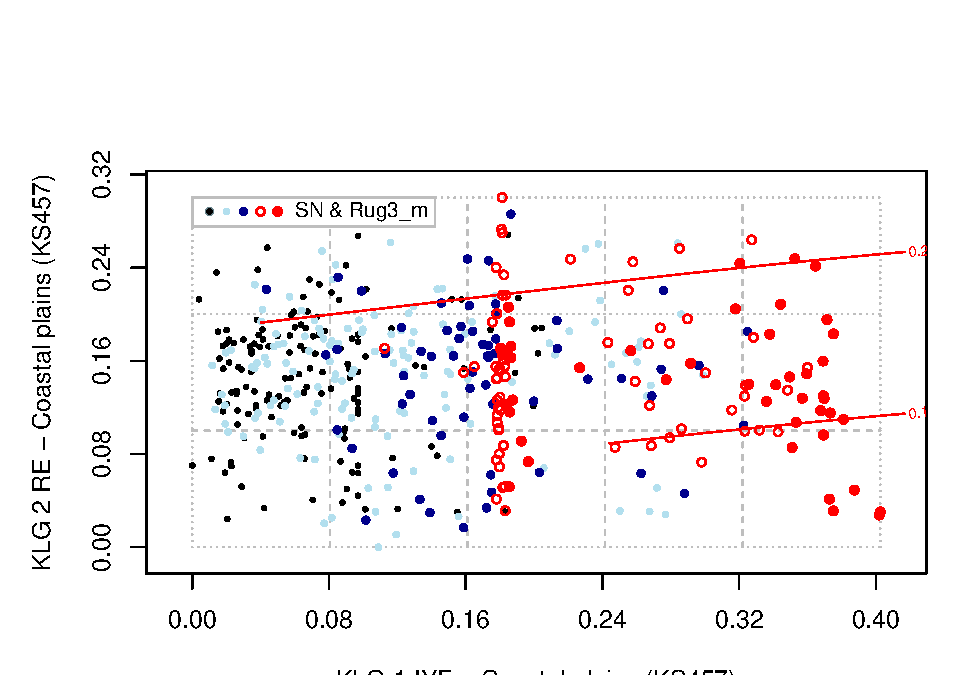
\includegraphics{Landscape_analysis_example_4_files/figure-latex/unnamed-chunk-47-1.pdf}

\begin{Shaded}
\begin{Highlighting}[]
\CommentTok{#Fig. 2. 1 IyK mot 3 VP; SN som symboler og isolinjer for Inns_s}

\CommentTok{#sONV'er som skal plottes mot hverandre}
\NormalTok{s1 <-}\StringTok{ }\NormalTok{sONV_IyK}
\NormalTok{s2 <-}\StringTok{ }\NormalTok{sONV_VP}

\CommentTok{#Finner koordinatene for hj?rner i det 'plotteomr?det' med koordinater (x1, x2, y1, y2) som gir}
\CommentTok{#like enheter p? begge akser. Vi holder x1, x2 og y1 faste og bestemmer y2 slik at (x2-x1)/(y2-y1) i plt=c(x1,x2,y1,y2)}
\CommentTok{#blir lik max(s1)/max(s2)}
\CommentTok{#Det krever at y2 = [(x2-x1)*max(s2) + y1*max(s1)]/max(s1) }
\CommentTok{#Setter vi x1, x2 og y1 konstante, f?r vi:}
\NormalTok{y2 <-}\StringTok{ }\NormalTok{(}\FloatTok{0.8}\OperatorTok{*}\KeywordTok{max}\NormalTok{(s2)}\OperatorTok{+}\FloatTok{0.15}\OperatorTok{*}\KeywordTok{max}\NormalTok{(s1))}\OperatorTok{/}\KeywordTok{max}\NormalTok{(s1)}
\CommentTok{#y2}

\KeywordTok{par}\NormalTok{(}\DataTypeTok{plt=}\KeywordTok{c}\NormalTok{(}\FloatTok{0.15}\NormalTok{, }\FloatTok{0.95}\NormalTok{, }\FloatTok{0.15}\NormalTok{, y2))}
\KeywordTok{plot}\NormalTok{(s1,s2,}\DataTypeTok{xlab=}\StringTok{"KLG 1 IYF - Coastal plains (KS457)"}\NormalTok{,}\DataTypeTok{ylab=}\StringTok{"KLG 3 VP - Coastal plains (KS457)"}\NormalTok{,}\DataTypeTok{xlim=}\KeywordTok{c}\NormalTok{(}\OperatorTok{-}\FloatTok{0.01}\NormalTok{,}\KeywordTok{max}\NormalTok{(s1)}\OperatorTok{+}\FloatTok{0.01}\NormalTok{),}\DataTypeTok{ylim=}\KeywordTok{c}\NormalTok{(}\OperatorTok{-}\FloatTok{0.01}\NormalTok{,}\KeywordTok{max}\NormalTok{(s2)}\OperatorTok{+}\FloatTok{0.01}\NormalTok{),}\DataTypeTok{xaxp=}\KeywordTok{c}\NormalTok{(}\DecValTok{0}\NormalTok{,}\FloatTok{0.4}\NormalTok{,}\DecValTok{5}\NormalTok{),}\DataTypeTok{yaxp=}\KeywordTok{c}\NormalTok{(}\DecValTok{0}\NormalTok{,}\FloatTok{0.4}\NormalTok{,}\DecValTok{5}\NormalTok{),}\DataTypeTok{type=}\StringTok{"n"}\NormalTok{) }\CommentTok{#Grunnlag for plotting av symboler etc.}
\KeywordTok{lines}\NormalTok{(}\KeywordTok{c}\NormalTok{(}\DecValTok{0}\NormalTok{,}\KeywordTok{max}\NormalTok{(s1)),}\KeywordTok{c}\NormalTok{(}\KeywordTok{max}\NormalTok{(s2),}\KeywordTok{max}\NormalTok{(s2)),}\DataTypeTok{lty=}\DecValTok{3}\NormalTok{,}\DataTypeTok{col=}\DecValTok{8}\NormalTok{)}
\KeywordTok{lines}\NormalTok{(}\KeywordTok{c}\NormalTok{(}\DecValTok{0}\NormalTok{,}\KeywordTok{max}\NormalTok{(s1)),}\KeywordTok{c}\NormalTok{(}\DecValTok{0}\NormalTok{,}\DecValTok{0}\NormalTok{),}\DataTypeTok{lty=}\DecValTok{3}\NormalTok{,}\DataTypeTok{col=}\DecValTok{8}\NormalTok{)}
\KeywordTok{lines}\NormalTok{(}\KeywordTok{c}\NormalTok{(}\DecValTok{0}\NormalTok{,}\DecValTok{0}\NormalTok{),}\KeywordTok{c}\NormalTok{(}\DecValTok{0}\NormalTok{,}\KeywordTok{max}\NormalTok{(s2)),}\DataTypeTok{lty=}\DecValTok{3}\NormalTok{,}\DataTypeTok{col=}\DecValTok{8}\NormalTok{)}
\KeywordTok{lines}\NormalTok{(}\KeywordTok{c}\NormalTok{(}\KeywordTok{max}\NormalTok{(s1),}\KeywordTok{max}\NormalTok{(s1)),}\KeywordTok{c}\NormalTok{(}\DecValTok{0}\NormalTok{,}\KeywordTok{max}\NormalTok{(s2)),}\DataTypeTok{lty=}\DecValTok{3}\NormalTok{,}\DataTypeTok{col=}\DecValTok{8}\NormalTok{)}

\KeywordTok{polygon}\NormalTok{(}\KeywordTok{c}\NormalTok{(}\DecValTok{4}\OperatorTok{*}\KeywordTok{max}\NormalTok{(s1)}\OperatorTok{/}\DecValTok{5}\NormalTok{,}\DecValTok{4}\OperatorTok{*}\KeywordTok{max}\NormalTok{(s1)}\OperatorTok{/}\DecValTok{5}\NormalTok{,}\KeywordTok{max}\NormalTok{(s1),}\KeywordTok{max}\NormalTok{(s1)),}\KeywordTok{c}\NormalTok{(}\KeywordTok{max}\NormalTok{(s2)}\OperatorTok{/}\DecValTok{2}\NormalTok{,}\KeywordTok{max}\NormalTok{(s2)}\OperatorTok{-}\FloatTok{0.025}\NormalTok{,}\KeywordTok{max}\NormalTok{(s2)}\OperatorTok{-}\FloatTok{0.025}\NormalTok{,}\KeywordTok{max}\NormalTok{(s2)}\OperatorTok{/}\DecValTok{2}\NormalTok{),}\DataTypeTok{col=}\StringTok{"lightgray"}\NormalTok{)}
\KeywordTok{polygon}\NormalTok{(}\KeywordTok{c}\NormalTok{(}\DecValTok{4}\OperatorTok{*}\KeywordTok{max}\NormalTok{(s1)}\OperatorTok{/}\DecValTok{5}\NormalTok{,}\DecValTok{4}\OperatorTok{*}\KeywordTok{max}\NormalTok{(s1)}\OperatorTok{/}\DecValTok{5}\NormalTok{,}\KeywordTok{max}\NormalTok{(s1),}\KeywordTok{max}\NormalTok{(s1)),}\KeywordTok{c}\NormalTok{(}\KeywordTok{max}\NormalTok{(s2)}\OperatorTok{/}\DecValTok{2}\NormalTok{,}\KeywordTok{max}\NormalTok{(s2)}\OperatorTok{-}\FloatTok{0.025}\NormalTok{,}\KeywordTok{max}\NormalTok{(s2)}\OperatorTok{-}\FloatTok{0.025}\NormalTok{,}\KeywordTok{max}\NormalTok{(s2)}\OperatorTok{/}\DecValTok{2}\NormalTok{),}\DataTypeTok{col=}\StringTok{"lightgray"}\NormalTok{,}\DataTypeTok{density=}\DecValTok{10}\NormalTok{) }\CommentTok{#legger egentlig et skr?tt raster opp?, og fjerner streken rundt}

\KeywordTok{lines}\NormalTok{(}\KeywordTok{c}\NormalTok{(}\DecValTok{0}\NormalTok{,}\KeywordTok{max}\NormalTok{(s1)),}\KeywordTok{c}\NormalTok{(}\KeywordTok{max}\NormalTok{(s2)}\OperatorTok{/}\DecValTok{2}\NormalTok{,}\KeywordTok{max}\NormalTok{(s2)}\OperatorTok{/}\DecValTok{2}\NormalTok{),}\DataTypeTok{lty=}\DecValTok{2}\NormalTok{,}\DataTypeTok{col=}\DecValTok{8}\NormalTok{)}
\KeywordTok{lines}\NormalTok{(}\KeywordTok{c}\NormalTok{(}\FloatTok{0.2}\OperatorTok{*}\KeywordTok{max}\NormalTok{(s1),}\FloatTok{0.2}\OperatorTok{*}\KeywordTok{max}\NormalTok{(s1)),}\KeywordTok{c}\NormalTok{(}\DecValTok{0}\NormalTok{,}\KeywordTok{max}\NormalTok{(s2)),}\DataTypeTok{lty=}\DecValTok{2}\NormalTok{,}\DataTypeTok{col=}\DecValTok{8}\NormalTok{)}
\KeywordTok{lines}\NormalTok{(}\KeywordTok{c}\NormalTok{(}\FloatTok{0.4}\OperatorTok{*}\KeywordTok{max}\NormalTok{(s1),}\FloatTok{0.4}\OperatorTok{*}\KeywordTok{max}\NormalTok{(s1)),}\KeywordTok{c}\NormalTok{(}\DecValTok{0}\NormalTok{,}\KeywordTok{max}\NormalTok{(s2)),}\DataTypeTok{lty=}\DecValTok{2}\NormalTok{,}\DataTypeTok{col=}\DecValTok{8}\NormalTok{)}
\KeywordTok{lines}\NormalTok{(}\KeywordTok{c}\NormalTok{(}\FloatTok{0.6}\OperatorTok{*}\KeywordTok{max}\NormalTok{(s1),}\FloatTok{0.6}\OperatorTok{*}\KeywordTok{max}\NormalTok{(s1)),}\KeywordTok{c}\NormalTok{(}\DecValTok{0}\NormalTok{,}\KeywordTok{max}\NormalTok{(s2)),}\DataTypeTok{lty=}\DecValTok{2}\NormalTok{,}\DataTypeTok{col=}\DecValTok{8}\NormalTok{)}
\KeywordTok{lines}\NormalTok{(}\KeywordTok{c}\NormalTok{(}\FloatTok{0.8}\OperatorTok{*}\KeywordTok{max}\NormalTok{(s1),}\FloatTok{0.8}\OperatorTok{*}\KeywordTok{max}\NormalTok{(s1)),}\KeywordTok{c}\NormalTok{(}\DecValTok{0}\NormalTok{,}\KeywordTok{max}\NormalTok{(s2)}\OperatorTok{-}\FloatTok{0.025}\NormalTok{),}\DataTypeTok{lty=}\DecValTok{2}\NormalTok{,}\DataTypeTok{col=}\DecValTok{8}\NormalTok{)}

\KeywordTok{lines}\NormalTok{(}\KeywordTok{c}\NormalTok{(}\KeywordTok{max}\NormalTok{(s1)}\OperatorTok{-}\FloatTok{0.14}\NormalTok{,}\KeywordTok{max}\NormalTok{(s1)),}\KeywordTok{c}\NormalTok{(}\KeywordTok{max}\NormalTok{(s2),}\KeywordTok{max}\NormalTok{(s2)),}\DataTypeTok{col=}\DecValTok{8}\NormalTok{)}
\KeywordTok{lines}\NormalTok{(}\KeywordTok{c}\NormalTok{(}\KeywordTok{max}\NormalTok{(s1)}\OperatorTok{-}\FloatTok{0.14}\NormalTok{,}\KeywordTok{max}\NormalTok{(s1)),}\KeywordTok{c}\NormalTok{(}\KeywordTok{max}\NormalTok{(s2)}\OperatorTok{-}\FloatTok{0.025}\NormalTok{,}\KeywordTok{max}\NormalTok{(s2)}\OperatorTok{-}\FloatTok{0.025}\NormalTok{),}\DataTypeTok{col=}\DecValTok{8}\NormalTok{)}
\KeywordTok{lines}\NormalTok{(}\KeywordTok{c}\NormalTok{(}\KeywordTok{max}\NormalTok{(s1)}\OperatorTok{-}\FloatTok{0.14}\NormalTok{,}\KeywordTok{max}\NormalTok{(s1)}\OperatorTok{-}\FloatTok{0.14}\NormalTok{),}\KeywordTok{c}\NormalTok{(}\KeywordTok{max}\NormalTok{(s2)}\OperatorTok{-}\FloatTok{0.025}\NormalTok{,}\KeywordTok{max}\NormalTok{(s2)),}\DataTypeTok{col=}\DecValTok{8}\NormalTok{)}
\KeywordTok{lines}\NormalTok{(}\KeywordTok{c}\NormalTok{(}\KeywordTok{max}\NormalTok{(s1),}\KeywordTok{max}\NormalTok{(s1)),}\KeywordTok{c}\NormalTok{(}\KeywordTok{max}\NormalTok{(s2)}\OperatorTok{-}\FloatTok{0.025}\NormalTok{,}\KeywordTok{max}\NormalTok{(s2)),}\DataTypeTok{col=}\DecValTok{8}\NormalTok{)}

\KeywordTok{text}\NormalTok{(}\KeywordTok{max}\NormalTok{(s1)}\OperatorTok{-}\FloatTok{0.075}\NormalTok{,}\KeywordTok{max}\NormalTok{(s2)}\OperatorTok{-}\FloatTok{0.012}\NormalTok{,}\StringTok{"SN & Inns_s"}\NormalTok{,}\DataTypeTok{adj=}\DecValTok{0}\NormalTok{,}\DataTypeTok{cex=}\FloatTok{0.8}\NormalTok{)}
\KeywordTok{points}\NormalTok{(}\KeywordTok{max}\NormalTok{(s1)}\OperatorTok{-}\FloatTok{0.13}\NormalTok{,}\KeywordTok{max}\NormalTok{(s2)}\OperatorTok{-}\FloatTok{0.012}\NormalTok{,}\DataTypeTok{pch=}\DecValTok{16}\NormalTok{,}\DataTypeTok{cex=}\FloatTok{0.5}\NormalTok{,}\DataTypeTok{col=}\StringTok{"black"}\NormalTok{)}
\KeywordTok{points}\NormalTok{(}\KeywordTok{max}\NormalTok{(s1)}\OperatorTok{-}\FloatTok{0.12}\NormalTok{,}\KeywordTok{max}\NormalTok{(s2)}\OperatorTok{-}\FloatTok{0.012}\NormalTok{,}\DataTypeTok{pch=}\DecValTok{16}\NormalTok{,}\DataTypeTok{cex=}\FloatTok{0.6}\NormalTok{,}\DataTypeTok{col=}\StringTok{"lightblue2"}\NormalTok{)}
\KeywordTok{points}\NormalTok{(}\KeywordTok{max}\NormalTok{(s1)}\OperatorTok{-}\FloatTok{0.11}\NormalTok{,}\KeywordTok{max}\NormalTok{(s2)}\OperatorTok{-}\FloatTok{0.012}\NormalTok{,}\DataTypeTok{pch=}\DecValTok{16}\NormalTok{,}\DataTypeTok{cex=}\FloatTok{0.75}\NormalTok{,}\DataTypeTok{col=}\StringTok{"darkblue"}\NormalTok{)}
\KeywordTok{points}\NormalTok{(}\KeywordTok{max}\NormalTok{(s1)}\OperatorTok{-}\FloatTok{0.10}\NormalTok{,}\KeywordTok{max}\NormalTok{(s2)}\OperatorTok{-}\FloatTok{0.012}\NormalTok{,}\DataTypeTok{pch=}\DecValTok{1}\NormalTok{,}\DataTypeTok{cex=}\FloatTok{0.75}\NormalTok{,}\DataTypeTok{col=}\StringTok{"red"}\NormalTok{)}
\KeywordTok{points}\NormalTok{(}\KeywordTok{max}\NormalTok{(s1)}\OperatorTok{-}\FloatTok{0.09}\NormalTok{,}\KeywordTok{max}\NormalTok{(s2)}\OperatorTok{-}\FloatTok{0.012}\NormalTok{,}\DataTypeTok{pch=}\DecValTok{16}\NormalTok{,}\DataTypeTok{cex=}\FloatTok{0.9}\NormalTok{,}\DataTypeTok{col=}\StringTok{"red"}\NormalTok{)}

\KeywordTok{points}\NormalTok{(s1[SN}\OperatorTok{==}\DecValTok{1}\NormalTok{],s2[SN}\OperatorTok{==}\DecValTok{1}\NormalTok{],}\DataTypeTok{pch=}\DecValTok{16}\NormalTok{,}\DataTypeTok{cex=}\FloatTok{0.5}\NormalTok{,}\DataTypeTok{col=}\DecValTok{1}\NormalTok{)}
\KeywordTok{points}\NormalTok{(s1[SN}\OperatorTok{==}\DecValTok{2}\NormalTok{],s2[SN}\OperatorTok{==}\DecValTok{2}\NormalTok{],}\DataTypeTok{pch=}\DecValTok{16}\NormalTok{,}\DataTypeTok{cex=}\FloatTok{0.6}\NormalTok{,}\DataTypeTok{col=}\StringTok{"lightblue2"}\NormalTok{)}
\KeywordTok{points}\NormalTok{(s1[SN}\OperatorTok{==}\DecValTok{3}\NormalTok{],s2[SN}\OperatorTok{==}\DecValTok{3}\NormalTok{],}\DataTypeTok{pch=}\DecValTok{16}\NormalTok{,}\DataTypeTok{cex=}\FloatTok{0.75}\NormalTok{,}\DataTypeTok{col=}\StringTok{"darkblue"}\NormalTok{)}
\KeywordTok{points}\NormalTok{(s1[SN}\OperatorTok{==}\DecValTok{4}\NormalTok{],s2[SN}\OperatorTok{==}\DecValTok{4}\NormalTok{],}\DataTypeTok{pch=}\DecValTok{1}\NormalTok{,}\DataTypeTok{cex=}\FloatTok{0.75}\NormalTok{,}\DataTypeTok{col=}\StringTok{"red"}\NormalTok{)}
\KeywordTok{points}\NormalTok{(s1[SN}\OperatorTok{==}\DecValTok{5}\NormalTok{],s2[SN}\OperatorTok{==}\DecValTok{5}\NormalTok{],}\DataTypeTok{pch=}\DecValTok{16}\NormalTok{,}\DataTypeTok{cex=}\FloatTok{0.9}\NormalTok{,}\DataTypeTok{col=}\StringTok{"red"}\NormalTok{)}

\NormalTok{os <-}\StringTok{ }\KeywordTok{ordisurf}\NormalTok{(snv[,}\KeywordTok{c}\NormalTok{(}\DecValTok{1}\NormalTok{,}\DecValTok{3}\NormalTok{)],Inns_s,}\DataTypeTok{display=}\StringTok{"sites"}\NormalTok{,}\DataTypeTok{levels=}\KeywordTok{c}\NormalTok{(}\FloatTok{0.1}\NormalTok{,}\FloatTok{0.2}\NormalTok{,}\FloatTok{0.3}\NormalTok{,}\FloatTok{0.4}\NormalTok{,}\FloatTok{0.5}\NormalTok{,}\FloatTok{0.6}\NormalTok{), }\DataTypeTok{col=}\StringTok{"red"}\NormalTok{,}\DataTypeTok{add=}\NormalTok{T) }\CommentTok{#inkluderer plotting p? eksisterende ordinasjonsdiagram}
\end{Highlighting}
\end{Shaded}

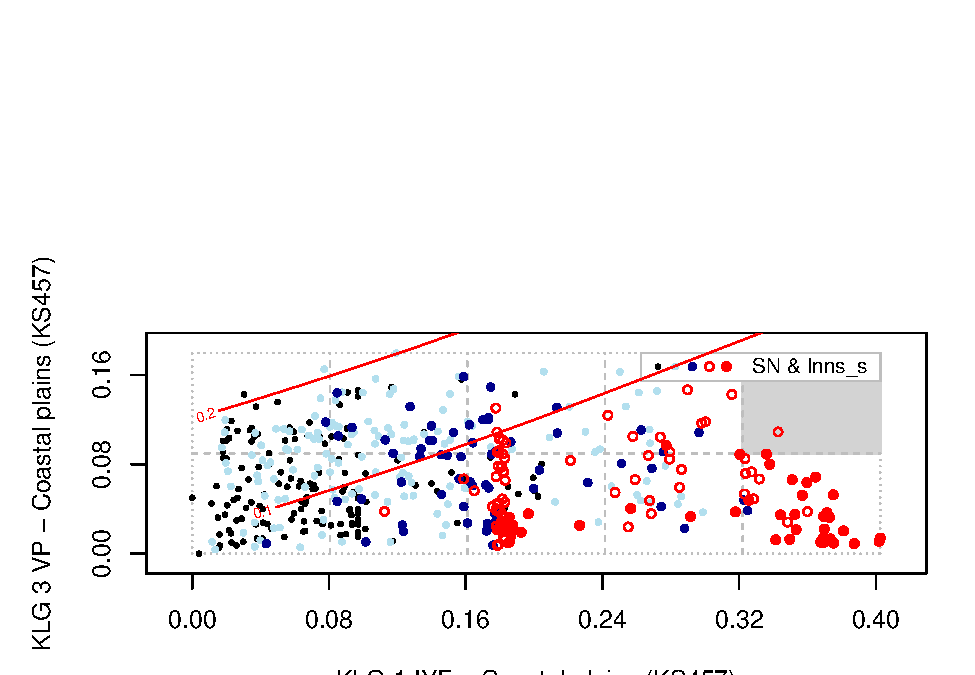
\includegraphics{Landscape_analysis_example_4_files/figure-latex/unnamed-chunk-48-1.pdf}

\begin{Shaded}
\begin{Highlighting}[]
\CommentTok{###}

\CommentTok{#1 IyK mot 3 VP; SN som symboler og isolinjer for Mire_a}

\KeywordTok{par}\NormalTok{(}\DataTypeTok{plt=}\KeywordTok{c}\NormalTok{(}\FloatTok{0.15}\NormalTok{, }\FloatTok{0.95}\NormalTok{, }\FloatTok{0.15}\NormalTok{, y2))}
\KeywordTok{plot}\NormalTok{(s1,s2,}\DataTypeTok{xlab=}\StringTok{"KLG 1 IYF - Coastal plains (KS457)"}\NormalTok{,}\DataTypeTok{ylab=}\StringTok{"KLG 3 VP - Coastal plains (KS457)"}\NormalTok{,}\DataTypeTok{xlim=}\KeywordTok{c}\NormalTok{(}\OperatorTok{-}\FloatTok{0.01}\NormalTok{,}\KeywordTok{max}\NormalTok{(s1)}\OperatorTok{+}\FloatTok{0.01}\NormalTok{),}\DataTypeTok{ylim=}\KeywordTok{c}\NormalTok{(}\OperatorTok{-}\FloatTok{0.01}\NormalTok{,}\KeywordTok{max}\NormalTok{(s2)}\OperatorTok{+}\FloatTok{0.01}\NormalTok{),}\DataTypeTok{xaxp=}\KeywordTok{c}\NormalTok{(}\DecValTok{0}\NormalTok{,}\FloatTok{0.4}\NormalTok{,}\DecValTok{5}\NormalTok{),}\DataTypeTok{yaxp=}\KeywordTok{c}\NormalTok{(}\DecValTok{0}\NormalTok{,}\FloatTok{0.4}\NormalTok{,}\DecValTok{5}\NormalTok{),}\DataTypeTok{type=}\StringTok{"n"}\NormalTok{) }\CommentTok{#Grunnlag for plotting av symboler etc.}
\KeywordTok{lines}\NormalTok{(}\KeywordTok{c}\NormalTok{(}\DecValTok{0}\NormalTok{,}\KeywordTok{max}\NormalTok{(s1)),}\KeywordTok{c}\NormalTok{(}\KeywordTok{max}\NormalTok{(s2),}\KeywordTok{max}\NormalTok{(s2)),}\DataTypeTok{lty=}\DecValTok{3}\NormalTok{,}\DataTypeTok{col=}\DecValTok{8}\NormalTok{)}
\KeywordTok{lines}\NormalTok{(}\KeywordTok{c}\NormalTok{(}\DecValTok{0}\NormalTok{,}\KeywordTok{max}\NormalTok{(s1)),}\KeywordTok{c}\NormalTok{(}\DecValTok{0}\NormalTok{,}\DecValTok{0}\NormalTok{),}\DataTypeTok{lty=}\DecValTok{3}\NormalTok{,}\DataTypeTok{col=}\DecValTok{8}\NormalTok{)}
\KeywordTok{lines}\NormalTok{(}\KeywordTok{c}\NormalTok{(}\DecValTok{0}\NormalTok{,}\DecValTok{0}\NormalTok{),}\KeywordTok{c}\NormalTok{(}\DecValTok{0}\NormalTok{,}\KeywordTok{max}\NormalTok{(s2)),}\DataTypeTok{lty=}\DecValTok{3}\NormalTok{,}\DataTypeTok{col=}\DecValTok{8}\NormalTok{)}
\KeywordTok{lines}\NormalTok{(}\KeywordTok{c}\NormalTok{(}\KeywordTok{max}\NormalTok{(s1),}\KeywordTok{max}\NormalTok{(s1)),}\KeywordTok{c}\NormalTok{(}\DecValTok{0}\NormalTok{,}\KeywordTok{max}\NormalTok{(s2)),}\DataTypeTok{lty=}\DecValTok{3}\NormalTok{,}\DataTypeTok{col=}\DecValTok{8}\NormalTok{)}

\KeywordTok{polygon}\NormalTok{(}\KeywordTok{c}\NormalTok{(}\DecValTok{4}\OperatorTok{*}\KeywordTok{max}\NormalTok{(s1)}\OperatorTok{/}\DecValTok{5}\NormalTok{,}\DecValTok{4}\OperatorTok{*}\KeywordTok{max}\NormalTok{(s1)}\OperatorTok{/}\DecValTok{5}\NormalTok{,}\KeywordTok{max}\NormalTok{(s1),}\KeywordTok{max}\NormalTok{(s1)),}\KeywordTok{c}\NormalTok{(}\KeywordTok{max}\NormalTok{(s2)}\OperatorTok{/}\DecValTok{2}\NormalTok{,}\KeywordTok{max}\NormalTok{(s2)}\OperatorTok{-}\FloatTok{0.025}\NormalTok{,}\KeywordTok{max}\NormalTok{(s2)}\OperatorTok{-}\FloatTok{0.025}\NormalTok{,}\KeywordTok{max}\NormalTok{(s2)}\OperatorTok{/}\DecValTok{2}\NormalTok{),}\DataTypeTok{col=}\StringTok{"lightgray"}\NormalTok{)}
\KeywordTok{polygon}\NormalTok{(}\KeywordTok{c}\NormalTok{(}\DecValTok{4}\OperatorTok{*}\KeywordTok{max}\NormalTok{(s1)}\OperatorTok{/}\DecValTok{5}\NormalTok{,}\DecValTok{4}\OperatorTok{*}\KeywordTok{max}\NormalTok{(s1)}\OperatorTok{/}\DecValTok{5}\NormalTok{,}\KeywordTok{max}\NormalTok{(s1),}\KeywordTok{max}\NormalTok{(s1)),}\KeywordTok{c}\NormalTok{(}\KeywordTok{max}\NormalTok{(s2)}\OperatorTok{/}\DecValTok{2}\NormalTok{,}\KeywordTok{max}\NormalTok{(s2)}\OperatorTok{-}\FloatTok{0.025}\NormalTok{,}\KeywordTok{max}\NormalTok{(s2)}\OperatorTok{-}\FloatTok{0.025}\NormalTok{,}\KeywordTok{max}\NormalTok{(s2)}\OperatorTok{/}\DecValTok{2}\NormalTok{),}\DataTypeTok{col=}\StringTok{"lightgray"}\NormalTok{,}\DataTypeTok{density=}\DecValTok{10}\NormalTok{) }\CommentTok{#legger egentlig et skr?tt raster opp?, og fjerner streken rundt}

\KeywordTok{lines}\NormalTok{(}\KeywordTok{c}\NormalTok{(}\DecValTok{0}\NormalTok{,}\KeywordTok{max}\NormalTok{(s1)),}\KeywordTok{c}\NormalTok{(}\KeywordTok{max}\NormalTok{(s2)}\OperatorTok{/}\DecValTok{2}\NormalTok{,}\KeywordTok{max}\NormalTok{(s2)}\OperatorTok{/}\DecValTok{2}\NormalTok{),}\DataTypeTok{lty=}\DecValTok{2}\NormalTok{,}\DataTypeTok{col=}\DecValTok{8}\NormalTok{)}
\KeywordTok{lines}\NormalTok{(}\KeywordTok{c}\NormalTok{(}\FloatTok{0.2}\OperatorTok{*}\KeywordTok{max}\NormalTok{(s1),}\FloatTok{0.2}\OperatorTok{*}\KeywordTok{max}\NormalTok{(s1)),}\KeywordTok{c}\NormalTok{(}\DecValTok{0}\NormalTok{,}\KeywordTok{max}\NormalTok{(s2)),}\DataTypeTok{lty=}\DecValTok{2}\NormalTok{,}\DataTypeTok{col=}\DecValTok{8}\NormalTok{)}
\KeywordTok{lines}\NormalTok{(}\KeywordTok{c}\NormalTok{(}\FloatTok{0.4}\OperatorTok{*}\KeywordTok{max}\NormalTok{(s1),}\FloatTok{0.4}\OperatorTok{*}\KeywordTok{max}\NormalTok{(s1)),}\KeywordTok{c}\NormalTok{(}\DecValTok{0}\NormalTok{,}\KeywordTok{max}\NormalTok{(s2)),}\DataTypeTok{lty=}\DecValTok{2}\NormalTok{,}\DataTypeTok{col=}\DecValTok{8}\NormalTok{)}
\KeywordTok{lines}\NormalTok{(}\KeywordTok{c}\NormalTok{(}\FloatTok{0.6}\OperatorTok{*}\KeywordTok{max}\NormalTok{(s1),}\FloatTok{0.6}\OperatorTok{*}\KeywordTok{max}\NormalTok{(s1)),}\KeywordTok{c}\NormalTok{(}\DecValTok{0}\NormalTok{,}\KeywordTok{max}\NormalTok{(s2)),}\DataTypeTok{lty=}\DecValTok{2}\NormalTok{,}\DataTypeTok{col=}\DecValTok{8}\NormalTok{)}
\KeywordTok{lines}\NormalTok{(}\KeywordTok{c}\NormalTok{(}\FloatTok{0.8}\OperatorTok{*}\KeywordTok{max}\NormalTok{(s1),}\FloatTok{0.8}\OperatorTok{*}\KeywordTok{max}\NormalTok{(s1)),}\KeywordTok{c}\NormalTok{(}\DecValTok{0}\NormalTok{,}\KeywordTok{max}\NormalTok{(s2)}\OperatorTok{-}\FloatTok{0.025}\NormalTok{),}\DataTypeTok{lty=}\DecValTok{2}\NormalTok{,}\DataTypeTok{col=}\DecValTok{8}\NormalTok{)}

\KeywordTok{lines}\NormalTok{(}\KeywordTok{c}\NormalTok{(}\KeywordTok{max}\NormalTok{(s1)}\OperatorTok{-}\FloatTok{0.14}\NormalTok{,}\KeywordTok{max}\NormalTok{(s1)),}\KeywordTok{c}\NormalTok{(}\KeywordTok{max}\NormalTok{(s2),}\KeywordTok{max}\NormalTok{(s2)),}\DataTypeTok{col=}\DecValTok{8}\NormalTok{)}
\KeywordTok{lines}\NormalTok{(}\KeywordTok{c}\NormalTok{(}\KeywordTok{max}\NormalTok{(s1)}\OperatorTok{-}\FloatTok{0.14}\NormalTok{,}\KeywordTok{max}\NormalTok{(s1)),}\KeywordTok{c}\NormalTok{(}\KeywordTok{max}\NormalTok{(s2)}\OperatorTok{-}\FloatTok{0.025}\NormalTok{,}\KeywordTok{max}\NormalTok{(s2)}\OperatorTok{-}\FloatTok{0.025}\NormalTok{),}\DataTypeTok{col=}\DecValTok{8}\NormalTok{)}
\KeywordTok{lines}\NormalTok{(}\KeywordTok{c}\NormalTok{(}\KeywordTok{max}\NormalTok{(s1)}\OperatorTok{-}\FloatTok{0.14}\NormalTok{,}\KeywordTok{max}\NormalTok{(s1)}\OperatorTok{-}\FloatTok{0.14}\NormalTok{),}\KeywordTok{c}\NormalTok{(}\KeywordTok{max}\NormalTok{(s2)}\OperatorTok{-}\FloatTok{0.025}\NormalTok{,}\KeywordTok{max}\NormalTok{(s2)),}\DataTypeTok{col=}\DecValTok{8}\NormalTok{)}
\KeywordTok{lines}\NormalTok{(}\KeywordTok{c}\NormalTok{(}\KeywordTok{max}\NormalTok{(s1),}\KeywordTok{max}\NormalTok{(s1)),}\KeywordTok{c}\NormalTok{(}\KeywordTok{max}\NormalTok{(s2)}\OperatorTok{-}\FloatTok{0.025}\NormalTok{,}\KeywordTok{max}\NormalTok{(s2)),}\DataTypeTok{col=}\DecValTok{8}\NormalTok{)}

\KeywordTok{text}\NormalTok{(}\KeywordTok{max}\NormalTok{(s1)}\OperatorTok{-}\FloatTok{0.075}\NormalTok{,}\KeywordTok{max}\NormalTok{(s2)}\OperatorTok{-}\FloatTok{0.012}\NormalTok{,}\StringTok{"SN & Mire_a"}\NormalTok{,}\DataTypeTok{adj=}\DecValTok{0}\NormalTok{,}\DataTypeTok{cex=}\FloatTok{0.8}\NormalTok{)}
\KeywordTok{points}\NormalTok{(}\KeywordTok{max}\NormalTok{(s1)}\OperatorTok{-}\FloatTok{0.13}\NormalTok{,}\KeywordTok{max}\NormalTok{(s2)}\OperatorTok{-}\FloatTok{0.012}\NormalTok{,}\DataTypeTok{pch=}\DecValTok{16}\NormalTok{,}\DataTypeTok{cex=}\FloatTok{0.5}\NormalTok{,}\DataTypeTok{col=}\StringTok{"black"}\NormalTok{)}
\KeywordTok{points}\NormalTok{(}\KeywordTok{max}\NormalTok{(s1)}\OperatorTok{-}\FloatTok{0.12}\NormalTok{,}\KeywordTok{max}\NormalTok{(s2)}\OperatorTok{-}\FloatTok{0.012}\NormalTok{,}\DataTypeTok{pch=}\DecValTok{16}\NormalTok{,}\DataTypeTok{cex=}\FloatTok{0.6}\NormalTok{,}\DataTypeTok{col=}\StringTok{"lightblue2"}\NormalTok{)}
\KeywordTok{points}\NormalTok{(}\KeywordTok{max}\NormalTok{(s1)}\OperatorTok{-}\FloatTok{0.11}\NormalTok{,}\KeywordTok{max}\NormalTok{(s2)}\OperatorTok{-}\FloatTok{0.012}\NormalTok{,}\DataTypeTok{pch=}\DecValTok{16}\NormalTok{,}\DataTypeTok{cex=}\FloatTok{0.75}\NormalTok{,}\DataTypeTok{col=}\StringTok{"darkblue"}\NormalTok{)}
\KeywordTok{points}\NormalTok{(}\KeywordTok{max}\NormalTok{(s1)}\OperatorTok{-}\FloatTok{0.10}\NormalTok{,}\KeywordTok{max}\NormalTok{(s2)}\OperatorTok{-}\FloatTok{0.012}\NormalTok{,}\DataTypeTok{pch=}\DecValTok{1}\NormalTok{,}\DataTypeTok{cex=}\FloatTok{0.75}\NormalTok{,}\DataTypeTok{col=}\StringTok{"red"}\NormalTok{)}
\KeywordTok{points}\NormalTok{(}\KeywordTok{max}\NormalTok{(s1)}\OperatorTok{-}\FloatTok{0.09}\NormalTok{,}\KeywordTok{max}\NormalTok{(s2)}\OperatorTok{-}\FloatTok{0.012}\NormalTok{,}\DataTypeTok{pch=}\DecValTok{16}\NormalTok{,}\DataTypeTok{cex=}\FloatTok{0.9}\NormalTok{,}\DataTypeTok{col=}\StringTok{"red"}\NormalTok{)}

\KeywordTok{points}\NormalTok{(s1[SN}\OperatorTok{==}\DecValTok{1}\NormalTok{],s2[SN}\OperatorTok{==}\DecValTok{1}\NormalTok{],}\DataTypeTok{pch=}\DecValTok{16}\NormalTok{,}\DataTypeTok{cex=}\FloatTok{0.5}\NormalTok{,}\DataTypeTok{col=}\DecValTok{1}\NormalTok{)}
\KeywordTok{points}\NormalTok{(s1[SN}\OperatorTok{==}\DecValTok{2}\NormalTok{],s2[SN}\OperatorTok{==}\DecValTok{2}\NormalTok{],}\DataTypeTok{pch=}\DecValTok{16}\NormalTok{,}\DataTypeTok{cex=}\FloatTok{0.6}\NormalTok{,}\DataTypeTok{col=}\StringTok{"lightblue2"}\NormalTok{)}
\KeywordTok{points}\NormalTok{(s1[SN}\OperatorTok{==}\DecValTok{3}\NormalTok{],s2[SN}\OperatorTok{==}\DecValTok{3}\NormalTok{],}\DataTypeTok{pch=}\DecValTok{16}\NormalTok{,}\DataTypeTok{cex=}\FloatTok{0.75}\NormalTok{,}\DataTypeTok{col=}\StringTok{"darkblue"}\NormalTok{)}
\KeywordTok{points}\NormalTok{(s1[SN}\OperatorTok{==}\DecValTok{4}\NormalTok{],s2[SN}\OperatorTok{==}\DecValTok{4}\NormalTok{],}\DataTypeTok{pch=}\DecValTok{1}\NormalTok{,}\DataTypeTok{cex=}\FloatTok{0.75}\NormalTok{,}\DataTypeTok{col=}\StringTok{"red"}\NormalTok{)}
\KeywordTok{points}\NormalTok{(s1[SN}\OperatorTok{==}\DecValTok{5}\NormalTok{],s2[SN}\OperatorTok{==}\DecValTok{5}\NormalTok{],}\DataTypeTok{pch=}\DecValTok{16}\NormalTok{,}\DataTypeTok{cex=}\FloatTok{0.9}\NormalTok{,}\DataTypeTok{col=}\StringTok{"red"}\NormalTok{)}

\NormalTok{os <-}\StringTok{ }\KeywordTok{ordisurf}\NormalTok{(snv[,}\KeywordTok{c}\NormalTok{(}\DecValTok{1}\NormalTok{,}\DecValTok{3}\NormalTok{)],Mire_a,}\DataTypeTok{display=}\StringTok{"sites"}\NormalTok{,}\DataTypeTok{levels=}\KeywordTok{c}\NormalTok{(}\FloatTok{0.05}\NormalTok{,}\FloatTok{0.1}\NormalTok{,}\FloatTok{0.2}\NormalTok{,}\FloatTok{0.3}\NormalTok{,}\FloatTok{0.4}\NormalTok{,}\FloatTok{0.5}\NormalTok{,}\FloatTok{0.6}\NormalTok{), }\DataTypeTok{col=}\StringTok{"red"}\NormalTok{,}\DataTypeTok{add=}\NormalTok{T) }\CommentTok{#inkluderer plotting p? eksisterende ordinasjonsdiagram}
\end{Highlighting}
\end{Shaded}

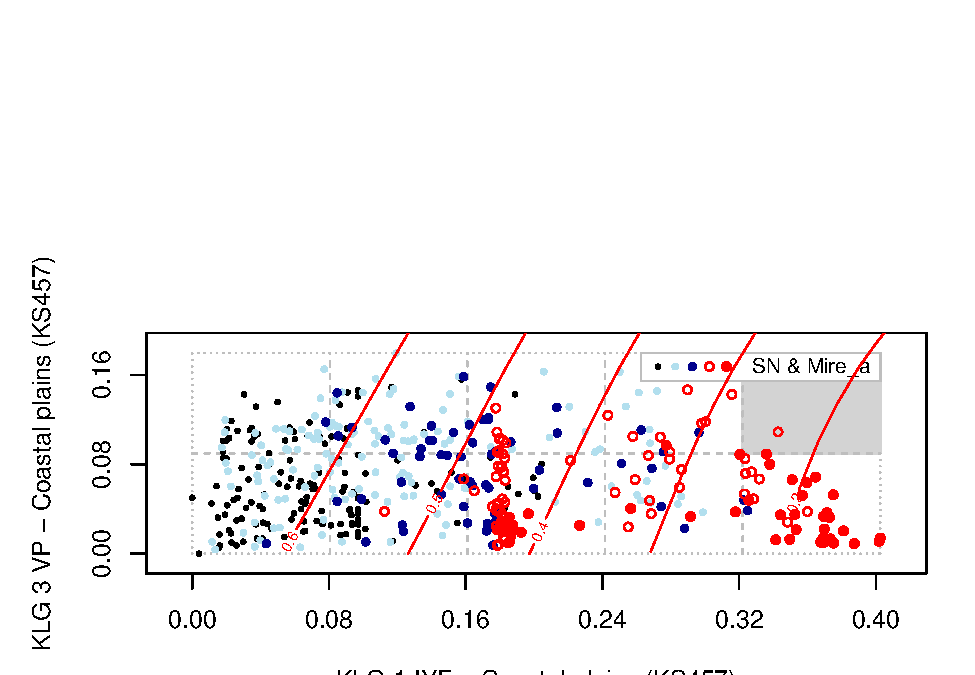
\includegraphics{Landscape_analysis_example_4_files/figure-latex/unnamed-chunk-49-1.pdf}

\begin{Shaded}
\begin{Highlighting}[]
\CommentTok{#Fig. 3. 2 RE mot 3 VP; SN som symboler og isolinjer for Inns_s}
\CommentTok{##Ikke relevant for siste gangs analyse}

\CommentTok{#sONV'er som skal plottes mot hverandre}
\NormalTok{s1 <-}\StringTok{ }\NormalTok{sONV_RE}
\NormalTok{s2 <-}\StringTok{ }\NormalTok{sONV_VP}

\CommentTok{#Finner koordinatene for hj?rner i det 'plotteomr?det' med koordinater (x1, x2, y1, y2) som gir}
\CommentTok{#like enheter p? begge akser. Vi holder x1, x2 og y1 faste og bestemmer y2 slik at (x2-x1)/(y2-y1) i plt=c(x1,x2,y1,y2)}
\CommentTok{#blir lik max(s1)/max(s2)}
\CommentTok{#Det krever at y2 = [(x2-x1)*max(s2) + y1*max(s1)]/max(s1) }
\CommentTok{#Setter vi x1, x2 og y1 konstante, f?r vi:}
\NormalTok{y2 <-}\StringTok{ }\NormalTok{(}\FloatTok{0.8}\OperatorTok{*}\KeywordTok{max}\NormalTok{(s2)}\OperatorTok{+}\FloatTok{0.15}\OperatorTok{*}\KeywordTok{max}\NormalTok{(s1))}\OperatorTok{/}\KeywordTok{max}\NormalTok{(s1)}
\NormalTok{y2}
\end{Highlighting}
\end{Shaded}

\begin{verbatim}
## [1] 0.6279221
\end{verbatim}

\begin{Shaded}
\begin{Highlighting}[]
\KeywordTok{par}\NormalTok{(}\DataTypeTok{plt=}\KeywordTok{c}\NormalTok{(}\FloatTok{0.15}\NormalTok{, }\FloatTok{0.95}\NormalTok{, }\FloatTok{0.15}\NormalTok{, y2))}
\KeywordTok{plot}\NormalTok{(s1,s2,}\DataTypeTok{xlab=}\StringTok{"KLG 2 RE - Coastal plains (KS457)"}\NormalTok{,}\DataTypeTok{ylab=}\StringTok{"KLG 3 VP - Coastal plains (KS457)"}\NormalTok{,}\DataTypeTok{xlim=}\KeywordTok{c}\NormalTok{(}\OperatorTok{-}\FloatTok{0.01}\NormalTok{,}\KeywordTok{max}\NormalTok{(s1)}\OperatorTok{+}\FloatTok{0.01}\NormalTok{),}\DataTypeTok{ylim=}\KeywordTok{c}\NormalTok{(}\OperatorTok{-}\FloatTok{0.01}\NormalTok{,}\KeywordTok{max}\NormalTok{(s2)}\OperatorTok{+}\FloatTok{0.01}\NormalTok{),}\DataTypeTok{xaxp=}\KeywordTok{c}\NormalTok{(}\DecValTok{0}\NormalTok{,}\FloatTok{0.4}\NormalTok{,}\DecValTok{5}\NormalTok{),}\DataTypeTok{yaxp=}\KeywordTok{c}\NormalTok{(}\DecValTok{0}\NormalTok{,}\FloatTok{0.4}\NormalTok{,}\DecValTok{5}\NormalTok{),}\DataTypeTok{type=}\StringTok{"n"}\NormalTok{) }\CommentTok{#Grunnlag for plotting av symboler etc.}
\KeywordTok{lines}\NormalTok{(}\KeywordTok{c}\NormalTok{(}\DecValTok{0}\NormalTok{,}\KeywordTok{max}\NormalTok{(s1)),}\KeywordTok{c}\NormalTok{(}\KeywordTok{max}\NormalTok{(s2),}\KeywordTok{max}\NormalTok{(s2)),}\DataTypeTok{lty=}\DecValTok{3}\NormalTok{,}\DataTypeTok{col=}\DecValTok{8}\NormalTok{)}
\KeywordTok{lines}\NormalTok{(}\KeywordTok{c}\NormalTok{(}\DecValTok{0}\NormalTok{,}\KeywordTok{max}\NormalTok{(s1)),}\KeywordTok{c}\NormalTok{(}\DecValTok{0}\NormalTok{,}\DecValTok{0}\NormalTok{),}\DataTypeTok{lty=}\DecValTok{3}\NormalTok{,}\DataTypeTok{col=}\DecValTok{8}\NormalTok{)}
\KeywordTok{lines}\NormalTok{(}\KeywordTok{c}\NormalTok{(}\DecValTok{0}\NormalTok{,}\DecValTok{0}\NormalTok{),}\KeywordTok{c}\NormalTok{(}\DecValTok{0}\NormalTok{,}\KeywordTok{max}\NormalTok{(s2)),}\DataTypeTok{lty=}\DecValTok{3}\NormalTok{,}\DataTypeTok{col=}\DecValTok{8}\NormalTok{)}
\KeywordTok{lines}\NormalTok{(}\KeywordTok{c}\NormalTok{(}\KeywordTok{max}\NormalTok{(s1),}\KeywordTok{max}\NormalTok{(s1)),}\KeywordTok{c}\NormalTok{(}\DecValTok{0}\NormalTok{,}\KeywordTok{max}\NormalTok{(s2)),}\DataTypeTok{lty=}\DecValTok{3}\NormalTok{,}\DataTypeTok{col=}\DecValTok{8}\NormalTok{)}

\KeywordTok{polygon}\NormalTok{(}\KeywordTok{c}\NormalTok{(}\KeywordTok{max}\NormalTok{(s1)}\OperatorTok{/}\DecValTok{2}\NormalTok{,}\KeywordTok{max}\NormalTok{(s1),}\KeywordTok{max}\NormalTok{(s1),}\KeywordTok{max}\NormalTok{(s1)}\OperatorTok{/}\DecValTok{2}\NormalTok{),}\KeywordTok{c}\NormalTok{(}\KeywordTok{max}\NormalTok{(s2)}\OperatorTok{/}\DecValTok{2}\NormalTok{,}\KeywordTok{max}\NormalTok{(s2)}\OperatorTok{/}\DecValTok{2}\NormalTok{,}\KeywordTok{max}\NormalTok{(s2),}\KeywordTok{max}\NormalTok{(s2)),}\DataTypeTok{col=}\StringTok{"lightgray"}\NormalTok{)}
\KeywordTok{polygon}\NormalTok{(}\KeywordTok{c}\NormalTok{(}\KeywordTok{max}\NormalTok{(s1)}\OperatorTok{/}\DecValTok{2}\NormalTok{,}\KeywordTok{max}\NormalTok{(s1),}\KeywordTok{max}\NormalTok{(s1),}\KeywordTok{max}\NormalTok{(s1)}\OperatorTok{/}\DecValTok{2}\NormalTok{),}\KeywordTok{c}\NormalTok{(}\KeywordTok{max}\NormalTok{(s2)}\OperatorTok{/}\DecValTok{2}\NormalTok{,}\KeywordTok{max}\NormalTok{(s2)}\OperatorTok{/}\DecValTok{2}\NormalTok{,}\KeywordTok{max}\NormalTok{(s2),}\KeywordTok{max}\NormalTok{(s2)),}\DataTypeTok{col=}\StringTok{"lightgray"}\NormalTok{,}\DataTypeTok{density=}\DecValTok{10}\NormalTok{) }\CommentTok{#legger egentlig et skr?tt raster opp?, og fjerner streken rundt}

\KeywordTok{lines}\NormalTok{(}\KeywordTok{c}\NormalTok{(}\DecValTok{0}\NormalTok{,}\KeywordTok{max}\NormalTok{(s1)),}\KeywordTok{c}\NormalTok{(}\KeywordTok{max}\NormalTok{(s2)}\OperatorTok{/}\DecValTok{2}\NormalTok{,}\KeywordTok{max}\NormalTok{(s2)}\OperatorTok{/}\DecValTok{2}\NormalTok{),}\DataTypeTok{lty=}\DecValTok{2}\NormalTok{,}\DataTypeTok{col=}\DecValTok{8}\NormalTok{)}
\KeywordTok{lines}\NormalTok{(}\KeywordTok{c}\NormalTok{(}\KeywordTok{max}\NormalTok{(s1)}\OperatorTok{/}\DecValTok{2}\NormalTok{,}\KeywordTok{max}\NormalTok{(s1)}\OperatorTok{/}\DecValTok{2}\NormalTok{),}\KeywordTok{c}\NormalTok{(}\DecValTok{0}\NormalTok{,}\KeywordTok{max}\NormalTok{(s2)),}\DataTypeTok{lty=}\DecValTok{2}\NormalTok{,}\DataTypeTok{col=}\DecValTok{8}\NormalTok{)}

\KeywordTok{lines}\NormalTok{(}\KeywordTok{c}\NormalTok{(}\DecValTok{0}\NormalTok{,}\FloatTok{0.095}\NormalTok{),}\KeywordTok{c}\NormalTok{(}\KeywordTok{max}\NormalTok{(s2),}\KeywordTok{max}\NormalTok{(s2)),}\DataTypeTok{col=}\DecValTok{8}\NormalTok{)}
\KeywordTok{lines}\NormalTok{(}\KeywordTok{c}\NormalTok{(}\DecValTok{0}\NormalTok{,}\FloatTok{0.095}\NormalTok{),}\KeywordTok{c}\NormalTok{(}\KeywordTok{max}\NormalTok{(s2)}\OperatorTok{-}\FloatTok{0.02}\NormalTok{,}\KeywordTok{max}\NormalTok{(s2)}\OperatorTok{-}\FloatTok{0.02}\NormalTok{),}\DataTypeTok{col=}\DecValTok{8}\NormalTok{)}
\KeywordTok{lines}\NormalTok{(}\KeywordTok{c}\NormalTok{(}\FloatTok{0.095}\NormalTok{,}\FloatTok{0.095}\NormalTok{),}\KeywordTok{c}\NormalTok{(}\KeywordTok{max}\NormalTok{(s2)}\OperatorTok{-}\FloatTok{0.02}\NormalTok{,}\KeywordTok{max}\NormalTok{(s2)),}\DataTypeTok{col=}\DecValTok{8}\NormalTok{)}
\KeywordTok{lines}\NormalTok{(}\KeywordTok{c}\NormalTok{(}\DecValTok{0}\NormalTok{,}\DecValTok{0}\NormalTok{),}\KeywordTok{c}\NormalTok{(}\KeywordTok{max}\NormalTok{(s2)}\OperatorTok{-}\FloatTok{0.02}\NormalTok{,}\KeywordTok{max}\NormalTok{(s2)),}\DataTypeTok{col=}\DecValTok{8}\NormalTok{)}

\KeywordTok{points}\NormalTok{(}\FloatTok{0.007}\NormalTok{,}\KeywordTok{max}\NormalTok{(s2)}\OperatorTok{-}\FloatTok{0.01}\NormalTok{,}\DataTypeTok{pch=}\DecValTok{16}\NormalTok{,}\DataTypeTok{cex=}\FloatTok{0.5}\NormalTok{,}\DataTypeTok{col=}\StringTok{"black"}\NormalTok{)}
\KeywordTok{points}\NormalTok{(}\FloatTok{0.014}\NormalTok{,}\KeywordTok{max}\NormalTok{(s2)}\OperatorTok{-}\FloatTok{0.01}\NormalTok{,}\DataTypeTok{pch=}\DecValTok{16}\NormalTok{,}\DataTypeTok{cex=}\FloatTok{0.6}\NormalTok{,}\DataTypeTok{col=}\StringTok{"lightblue2"}\NormalTok{)}
\KeywordTok{points}\NormalTok{(}\FloatTok{0.021}\NormalTok{,}\KeywordTok{max}\NormalTok{(s2)}\OperatorTok{-}\FloatTok{0.01}\NormalTok{,}\DataTypeTok{pch=}\DecValTok{16}\NormalTok{,}\DataTypeTok{cex=}\FloatTok{0.75}\NormalTok{,}\DataTypeTok{col=}\StringTok{"darkblue"}\NormalTok{)}
\KeywordTok{points}\NormalTok{(}\FloatTok{0.028}\NormalTok{,}\KeywordTok{max}\NormalTok{(s2)}\OperatorTok{-}\FloatTok{0.01}\NormalTok{,}\DataTypeTok{pch=}\DecValTok{1}\NormalTok{,}\DataTypeTok{cex=}\FloatTok{0.75}\NormalTok{,}\DataTypeTok{col=}\StringTok{"red"}\NormalTok{)}
\KeywordTok{points}\NormalTok{(}\FloatTok{0.035}\NormalTok{,}\KeywordTok{max}\NormalTok{(s2)}\OperatorTok{-}\FloatTok{0.01}\NormalTok{,}\DataTypeTok{pch=}\DecValTok{16}\NormalTok{,}\DataTypeTok{cex=}\FloatTok{0.9}\NormalTok{,}\DataTypeTok{col=}\StringTok{"red"}\NormalTok{)}

\KeywordTok{text}\NormalTok{(}\FloatTok{0.045}\NormalTok{,}\KeywordTok{max}\NormalTok{(s2)}\OperatorTok{-}\FloatTok{0.01}\NormalTok{,}\StringTok{"SN & Inns_s"}\NormalTok{,}\DataTypeTok{adj=}\DecValTok{0}\NormalTok{,}\DataTypeTok{cex=}\FloatTok{0.8}\NormalTok{)}
\KeywordTok{points}\NormalTok{(s1[SN}\OperatorTok{==}\DecValTok{1}\NormalTok{],s2[SN}\OperatorTok{==}\DecValTok{1}\NormalTok{],}\DataTypeTok{pch=}\DecValTok{16}\NormalTok{,}\DataTypeTok{cex=}\FloatTok{0.5}\NormalTok{,}\DataTypeTok{col=}\DecValTok{1}\NormalTok{)}
\KeywordTok{points}\NormalTok{(s1[SN}\OperatorTok{==}\DecValTok{2}\NormalTok{],s2[SN}\OperatorTok{==}\DecValTok{2}\NormalTok{],}\DataTypeTok{pch=}\DecValTok{16}\NormalTok{,}\DataTypeTok{cex=}\FloatTok{0.6}\NormalTok{,}\DataTypeTok{col=}\StringTok{"lightblue2"}\NormalTok{)}
\KeywordTok{points}\NormalTok{(s1[SN}\OperatorTok{==}\DecValTok{3}\NormalTok{],s2[SN}\OperatorTok{==}\DecValTok{3}\NormalTok{],}\DataTypeTok{pch=}\DecValTok{16}\NormalTok{,}\DataTypeTok{cex=}\FloatTok{0.75}\NormalTok{,}\DataTypeTok{col=}\StringTok{"darkblue"}\NormalTok{)}
\KeywordTok{points}\NormalTok{(s1[SN}\OperatorTok{==}\DecValTok{4}\NormalTok{],s2[SN}\OperatorTok{==}\DecValTok{4}\NormalTok{],}\DataTypeTok{pch=}\DecValTok{1}\NormalTok{,}\DataTypeTok{cex=}\FloatTok{0.75}\NormalTok{,}\DataTypeTok{col=}\StringTok{"red"}\NormalTok{)}
\KeywordTok{points}\NormalTok{(s1[SN}\OperatorTok{==}\DecValTok{5}\NormalTok{],s2[SN}\OperatorTok{==}\DecValTok{5}\NormalTok{],}\DataTypeTok{pch=}\DecValTok{16}\NormalTok{,}\DataTypeTok{cex=}\FloatTok{0.9}\NormalTok{,}\DataTypeTok{col=}\StringTok{"red"}\NormalTok{)}

\NormalTok{os <-}\StringTok{ }\KeywordTok{ordisurf}\NormalTok{(snv[,}\KeywordTok{c}\NormalTok{(}\DecValTok{1}\NormalTok{,}\DecValTok{2}\NormalTok{)],Inns_s,}\DataTypeTok{display=}\StringTok{"sites"}\NormalTok{,}\DataTypeTok{levels=}\KeywordTok{c}\NormalTok{(}\FloatTok{0.1}\NormalTok{,}\FloatTok{0.2}\NormalTok{,}\FloatTok{0.3}\NormalTok{,}\FloatTok{0.4}\NormalTok{,}\FloatTok{0.5}\NormalTok{,}\FloatTok{0.6}\NormalTok{,}\FloatTok{0.7}\NormalTok{), }\DataTypeTok{col=}\StringTok{"red"}\NormalTok{,}\DataTypeTok{add=}\NormalTok{T) }\CommentTok{#inkluderer plotting p? eksisterende ordinasjonsdiagram}
\end{Highlighting}
\end{Shaded}

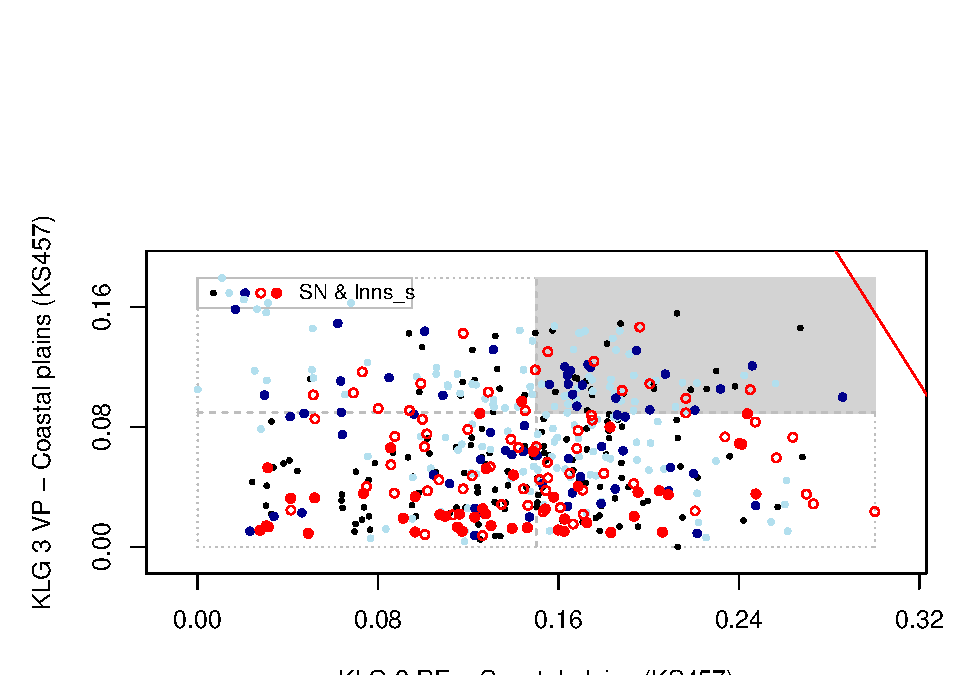
\includegraphics{Landscape_analysis_example_4_files/figure-latex/unnamed-chunk-50-1.pdf}

\begin{Shaded}
\begin{Highlighting}[]
\CommentTok{###}

\CommentTok{#Fig. 4. 1 IyK mot 4 SgP; SN som symboler og isolinjer for Maro_s ##Ikke relevant for siste gangs analyse}

\CommentTok{#sONV'er som skal plottes mot hverandre}
\NormalTok{s1 <-}\StringTok{ }\NormalTok{sONV_IyK}
\CommentTok{#s2 <- sONV_SgP}

\CommentTok{#Finner koordinatene for hj?rner i det 'plotteomr?det' med koordinater (x1, x2, y1, y2) som gir}
\CommentTok{#like enheter p? begge akser. Vi holder x1, x2 og y1 faste og bestemmer y2 slik at (x2-x1)/(y2-y1) i plt=c(x1,x2,y1,y2)}
\CommentTok{#blir lik max(s1)/max(s2)}
\CommentTok{#Det krever at y2 = [(x2-x1)*max(s2) + y1*max(s1)]/max(s1) }
\CommentTok{#Setter vi x1, x2 og y1 konstante, f?r vi:}
\NormalTok{y2 <-}\StringTok{ }\NormalTok{(}\FloatTok{0.8}\OperatorTok{*}\KeywordTok{max}\NormalTok{(s2)}\OperatorTok{+}\FloatTok{0.15}\OperatorTok{*}\KeywordTok{max}\NormalTok{(s1))}\OperatorTok{/}\KeywordTok{max}\NormalTok{(s1)}
\CommentTok{#y2}

\KeywordTok{par}\NormalTok{(}\DataTypeTok{plt=}\KeywordTok{c}\NormalTok{(}\FloatTok{0.15}\NormalTok{, }\FloatTok{0.95}\NormalTok{, }\FloatTok{0.15}\NormalTok{, y2))}
\KeywordTok{plot}\NormalTok{(s1,s2,}\DataTypeTok{xlab=}\StringTok{"KLG 1 IYF - Coastal plains (KS457)"}\NormalTok{,}\DataTypeTok{ylab=}\StringTok{"KLG 4 SgP - Coastal plains (KS457)"}\NormalTok{,}\DataTypeTok{xlim=}\KeywordTok{c}\NormalTok{(}\OperatorTok{-}\FloatTok{0.01}\NormalTok{,}\KeywordTok{max}\NormalTok{(s1)}\OperatorTok{+}\FloatTok{0.01}\NormalTok{),}\DataTypeTok{ylim=}\KeywordTok{c}\NormalTok{(}\OperatorTok{-}\FloatTok{0.01}\NormalTok{,}\KeywordTok{max}\NormalTok{(s2)}\OperatorTok{+}\FloatTok{0.01}\NormalTok{),}\DataTypeTok{xaxp=}\KeywordTok{c}\NormalTok{(}\DecValTok{0}\NormalTok{,}\FloatTok{0.4}\NormalTok{,}\DecValTok{5}\NormalTok{),}\DataTypeTok{yaxp=}\KeywordTok{c}\NormalTok{(}\DecValTok{0}\NormalTok{,}\FloatTok{0.4}\NormalTok{,}\DecValTok{5}\NormalTok{),}\DataTypeTok{type=}\StringTok{"n"}\NormalTok{) }\CommentTok{#Grunnlag for plotting av symboler etc.}
\KeywordTok{lines}\NormalTok{(}\KeywordTok{c}\NormalTok{(}\DecValTok{0}\NormalTok{,}\KeywordTok{max}\NormalTok{(s1)),}\KeywordTok{c}\NormalTok{(}\KeywordTok{max}\NormalTok{(s2),}\KeywordTok{max}\NormalTok{(s2)),}\DataTypeTok{lty=}\DecValTok{3}\NormalTok{,}\DataTypeTok{col=}\DecValTok{8}\NormalTok{)}
\KeywordTok{lines}\NormalTok{(}\KeywordTok{c}\NormalTok{(}\DecValTok{0}\NormalTok{,}\KeywordTok{max}\NormalTok{(s1)),}\KeywordTok{c}\NormalTok{(}\DecValTok{0}\NormalTok{,}\DecValTok{0}\NormalTok{),}\DataTypeTok{lty=}\DecValTok{3}\NormalTok{,}\DataTypeTok{col=}\DecValTok{8}\NormalTok{)}
\KeywordTok{lines}\NormalTok{(}\KeywordTok{c}\NormalTok{(}\DecValTok{0}\NormalTok{,}\DecValTok{0}\NormalTok{),}\KeywordTok{c}\NormalTok{(}\DecValTok{0}\NormalTok{,}\KeywordTok{max}\NormalTok{(s2)),}\DataTypeTok{lty=}\DecValTok{3}\NormalTok{,}\DataTypeTok{col=}\DecValTok{8}\NormalTok{)}
\KeywordTok{lines}\NormalTok{(}\KeywordTok{c}\NormalTok{(}\KeywordTok{max}\NormalTok{(s1),}\KeywordTok{max}\NormalTok{(s1)),}\KeywordTok{c}\NormalTok{(}\DecValTok{0}\NormalTok{,}\KeywordTok{max}\NormalTok{(s2)),}\DataTypeTok{lty=}\DecValTok{3}\NormalTok{,}\DataTypeTok{col=}\DecValTok{8}\NormalTok{)}

\KeywordTok{polygon}\NormalTok{(}\KeywordTok{c}\NormalTok{(}\DecValTok{0}\NormalTok{,}\DecValTok{0}\NormalTok{,}\FloatTok{0.8}\OperatorTok{*}\KeywordTok{max}\NormalTok{(s1),}\FloatTok{0.8}\OperatorTok{*}\KeywordTok{max}\NormalTok{(s1)),}\KeywordTok{c}\NormalTok{(}\DecValTok{0}\NormalTok{,}\KeywordTok{max}\NormalTok{(s2)}\OperatorTok{/}\DecValTok{2}\NormalTok{,}\KeywordTok{max}\NormalTok{(s2)}\OperatorTok{/}\DecValTok{2}\NormalTok{,}\DecValTok{0}\NormalTok{),}\DataTypeTok{col=}\StringTok{"lightgray"}\NormalTok{)}
\KeywordTok{polygon}\NormalTok{(}\KeywordTok{c}\NormalTok{(}\DecValTok{0}\NormalTok{,}\DecValTok{0}\NormalTok{,}\FloatTok{0.8}\OperatorTok{*}\KeywordTok{max}\NormalTok{(s1),}\FloatTok{0.8}\OperatorTok{*}\KeywordTok{max}\NormalTok{(s1)),}\KeywordTok{c}\NormalTok{(}\DecValTok{0}\NormalTok{,}\KeywordTok{max}\NormalTok{(s2)}\OperatorTok{/}\DecValTok{2}\NormalTok{,}\KeywordTok{max}\NormalTok{(s2)}\OperatorTok{/}\DecValTok{2}\NormalTok{,}\DecValTok{0}\NormalTok{),}\DataTypeTok{col=}\StringTok{"lightgray"}\NormalTok{,}\DataTypeTok{density=}\DecValTok{10}\NormalTok{) }\CommentTok{#legger egentlig et skr?tt raster opp?, og fjerner streken rundt}

\KeywordTok{lines}\NormalTok{(}\KeywordTok{c}\NormalTok{(}\DecValTok{0}\NormalTok{,}\KeywordTok{max}\NormalTok{(s1)),}\KeywordTok{c}\NormalTok{(}\KeywordTok{max}\NormalTok{(s2)}\OperatorTok{/}\DecValTok{2}\NormalTok{,}\KeywordTok{max}\NormalTok{(s2)}\OperatorTok{/}\DecValTok{2}\NormalTok{),}\DataTypeTok{lty=}\DecValTok{2}\NormalTok{,}\DataTypeTok{col=}\DecValTok{8}\NormalTok{)}
\KeywordTok{lines}\NormalTok{(}\KeywordTok{c}\NormalTok{(}\FloatTok{0.2}\OperatorTok{*}\KeywordTok{max}\NormalTok{(s1),}\FloatTok{0.2}\OperatorTok{*}\KeywordTok{max}\NormalTok{(s1)),}\KeywordTok{c}\NormalTok{(}\FloatTok{0.025}\NormalTok{,}\KeywordTok{max}\NormalTok{(s2)),}\DataTypeTok{lty=}\DecValTok{2}\NormalTok{,}\DataTypeTok{col=}\DecValTok{8}\NormalTok{)}
\KeywordTok{lines}\NormalTok{(}\KeywordTok{c}\NormalTok{(}\FloatTok{0.4}\OperatorTok{*}\KeywordTok{max}\NormalTok{(s1),}\FloatTok{0.4}\OperatorTok{*}\KeywordTok{max}\NormalTok{(s1)),}\KeywordTok{c}\NormalTok{(}\DecValTok{0}\NormalTok{,}\KeywordTok{max}\NormalTok{(s2)),}\DataTypeTok{lty=}\DecValTok{2}\NormalTok{,}\DataTypeTok{col=}\DecValTok{8}\NormalTok{)}
\KeywordTok{lines}\NormalTok{(}\KeywordTok{c}\NormalTok{(}\FloatTok{0.6}\OperatorTok{*}\KeywordTok{max}\NormalTok{(s1),}\FloatTok{0.6}\OperatorTok{*}\KeywordTok{max}\NormalTok{(s1)),}\KeywordTok{c}\NormalTok{(}\DecValTok{0}\NormalTok{,}\KeywordTok{max}\NormalTok{(s2)),}\DataTypeTok{lty=}\DecValTok{2}\NormalTok{,}\DataTypeTok{col=}\DecValTok{8}\NormalTok{)}
\KeywordTok{lines}\NormalTok{(}\KeywordTok{c}\NormalTok{(}\FloatTok{0.8}\OperatorTok{*}\KeywordTok{max}\NormalTok{(s1),}\FloatTok{0.8}\OperatorTok{*}\KeywordTok{max}\NormalTok{(s1)),}\KeywordTok{c}\NormalTok{(}\DecValTok{0}\NormalTok{,}\KeywordTok{max}\NormalTok{(s2)),}\DataTypeTok{lty=}\DecValTok{2}\NormalTok{,}\DataTypeTok{col=}\DecValTok{8}\NormalTok{)}

\KeywordTok{polygon}\NormalTok{(}\KeywordTok{c}\NormalTok{(}\DecValTok{0}\NormalTok{,}\DecValTok{0}\NormalTok{,}\FloatTok{0.142}\NormalTok{,}\FloatTok{0.142}\NormalTok{),}\KeywordTok{c}\NormalTok{(}\DecValTok{0}\NormalTok{,}\FloatTok{0.025}\NormalTok{,}\FloatTok{0.025}\NormalTok{,}\DecValTok{0}\NormalTok{),}\DataTypeTok{col=}\StringTok{"white"}\NormalTok{)}
\KeywordTok{polygon}\NormalTok{(}\KeywordTok{c}\NormalTok{(}\DecValTok{0}\NormalTok{,}\DecValTok{0}\NormalTok{,}\FloatTok{0.142}\NormalTok{,}\FloatTok{0.142}\NormalTok{),}\KeywordTok{c}\NormalTok{(}\DecValTok{0}\NormalTok{,}\FloatTok{0.025}\NormalTok{,}\FloatTok{0.025}\NormalTok{,}\DecValTok{0}\NormalTok{),}\DataTypeTok{col=}\StringTok{"white"}\NormalTok{,}\DataTypeTok{density=}\DecValTok{10}\NormalTok{) }\CommentTok{#legger egentlig et skr?tt raster opp?, og fjerner streken rundt}

\KeywordTok{lines}\NormalTok{(}\KeywordTok{c}\NormalTok{(}\DecValTok{0}\NormalTok{,}\FloatTok{0.142}\NormalTok{),}\KeywordTok{c}\NormalTok{(}\DecValTok{0}\NormalTok{,}\DecValTok{0}\NormalTok{),}\DataTypeTok{col=}\DecValTok{8}\NormalTok{)}
\KeywordTok{lines}\NormalTok{(}\KeywordTok{c}\NormalTok{(}\DecValTok{0}\NormalTok{,}\FloatTok{0.142}\NormalTok{),}\KeywordTok{c}\NormalTok{(}\FloatTok{0.025}\NormalTok{,}\FloatTok{0.025}\NormalTok{),}\DataTypeTok{col=}\DecValTok{8}\NormalTok{)}
\KeywordTok{lines}\NormalTok{(}\KeywordTok{c}\NormalTok{(}\DecValTok{0}\NormalTok{,}\DecValTok{0}\NormalTok{),}\KeywordTok{c}\NormalTok{(}\DecValTok{0}\NormalTok{,}\FloatTok{0.025}\NormalTok{),}\DataTypeTok{col=}\DecValTok{8}\NormalTok{)}
\KeywordTok{lines}\NormalTok{(}\KeywordTok{c}\NormalTok{(}\FloatTok{0.142}\NormalTok{,}\FloatTok{0.142}\NormalTok{),}\KeywordTok{c}\NormalTok{(}\DecValTok{0}\NormalTok{,}\FloatTok{0.025}\NormalTok{),}\DataTypeTok{col=}\DecValTok{8}\NormalTok{)}

\KeywordTok{points}\NormalTok{(}\FloatTok{0.01}\NormalTok{,}\FloatTok{0.012}\NormalTok{,}\DataTypeTok{pch=}\DecValTok{16}\NormalTok{,}\DataTypeTok{cex=}\FloatTok{0.5}\NormalTok{,}\DataTypeTok{col=}\StringTok{"black"}\NormalTok{)}
\KeywordTok{points}\NormalTok{(}\FloatTok{0.02}\NormalTok{,}\FloatTok{0.012}\NormalTok{,}\DataTypeTok{pch=}\DecValTok{16}\NormalTok{,}\DataTypeTok{cex=}\FloatTok{0.6}\NormalTok{,}\DataTypeTok{col=}\StringTok{"lightblue2"}\NormalTok{)}
\KeywordTok{points}\NormalTok{(}\FloatTok{0.03}\NormalTok{,}\FloatTok{0.012}\NormalTok{,}\DataTypeTok{pch=}\DecValTok{16}\NormalTok{,}\DataTypeTok{cex=}\FloatTok{0.75}\NormalTok{,}\DataTypeTok{col=}\StringTok{"darkblue"}\NormalTok{)}
\KeywordTok{points}\NormalTok{(}\FloatTok{0.04}\NormalTok{,}\FloatTok{0.012}\NormalTok{,}\DataTypeTok{pch=}\DecValTok{1}\NormalTok{,}\DataTypeTok{cex=}\FloatTok{0.75}\NormalTok{,}\DataTypeTok{col=}\StringTok{"red"}\NormalTok{)}
\KeywordTok{points}\NormalTok{(}\FloatTok{0.05}\NormalTok{,}\FloatTok{0.012}\NormalTok{,}\DataTypeTok{pch=}\DecValTok{16}\NormalTok{,}\DataTypeTok{cex=}\FloatTok{0.9}\NormalTok{,}\DataTypeTok{col=}\StringTok{"red"}\NormalTok{)}

\KeywordTok{text}\NormalTok{(}\FloatTok{0.06}\NormalTok{,}\FloatTok{0.012}\NormalTok{,}\StringTok{"SN & Maro_s"}\NormalTok{,}\DataTypeTok{adj=}\DecValTok{0}\NormalTok{,}\DataTypeTok{cex=}\FloatTok{0.8}\NormalTok{)}
\KeywordTok{points}\NormalTok{(s1[SN}\OperatorTok{==}\DecValTok{1}\NormalTok{],s2[SN}\OperatorTok{==}\DecValTok{1}\NormalTok{],}\DataTypeTok{pch=}\DecValTok{16}\NormalTok{,}\DataTypeTok{cex=}\FloatTok{0.5}\NormalTok{,}\DataTypeTok{col=}\DecValTok{1}\NormalTok{)}
\KeywordTok{points}\NormalTok{(s1[SN}\OperatorTok{==}\DecValTok{2}\NormalTok{],s2[SN}\OperatorTok{==}\DecValTok{2}\NormalTok{],}\DataTypeTok{pch=}\DecValTok{16}\NormalTok{,}\DataTypeTok{cex=}\FloatTok{0.6}\NormalTok{,}\DataTypeTok{col=}\StringTok{"lightblue2"}\NormalTok{)}
\KeywordTok{points}\NormalTok{(s1[SN}\OperatorTok{==}\DecValTok{3}\NormalTok{],s2[SN}\OperatorTok{==}\DecValTok{3}\NormalTok{],}\DataTypeTok{pch=}\DecValTok{16}\NormalTok{,}\DataTypeTok{cex=}\FloatTok{0.75}\NormalTok{,}\DataTypeTok{col=}\StringTok{"darkblue"}\NormalTok{)}
\KeywordTok{points}\NormalTok{(s1[SN}\OperatorTok{==}\DecValTok{4}\NormalTok{],s2[SN}\OperatorTok{==}\DecValTok{4}\NormalTok{],}\DataTypeTok{pch=}\DecValTok{1}\NormalTok{,}\DataTypeTok{cex=}\FloatTok{0.75}\NormalTok{,}\DataTypeTok{col=}\StringTok{"red"}\NormalTok{)}
\KeywordTok{points}\NormalTok{(s1[SN}\OperatorTok{==}\DecValTok{5}\NormalTok{],s2[SN}\OperatorTok{==}\DecValTok{5}\NormalTok{],}\DataTypeTok{pch=}\DecValTok{16}\NormalTok{,}\DataTypeTok{cex=}\FloatTok{0.9}\NormalTok{,}\DataTypeTok{col=}\StringTok{"red"}\NormalTok{)}

\NormalTok{os <-}\StringTok{ }\KeywordTok{ordisurf}\NormalTok{(snv[,}\KeywordTok{c}\NormalTok{(}\DecValTok{1}\NormalTok{,}\DecValTok{4}\NormalTok{)],Maro_s,}\DataTypeTok{display=}\StringTok{"sites"}\NormalTok{,}\DataTypeTok{levels=}\KeywordTok{c}\NormalTok{(}\FloatTok{0.1}\NormalTok{,}\FloatTok{0.2}\NormalTok{,}\FloatTok{0.3}\NormalTok{,}\FloatTok{0.4}\NormalTok{,}\FloatTok{0.5}\NormalTok{,}\FloatTok{0.6}\NormalTok{,}\FloatTok{0.7}\NormalTok{), }\DataTypeTok{col=}\StringTok{"red"}\NormalTok{,}\DataTypeTok{add=}\NormalTok{T) }\CommentTok{#inkluderer plotting p? eksisterende ordinasjonsdiagram}
\end{Highlighting}
\end{Shaded}

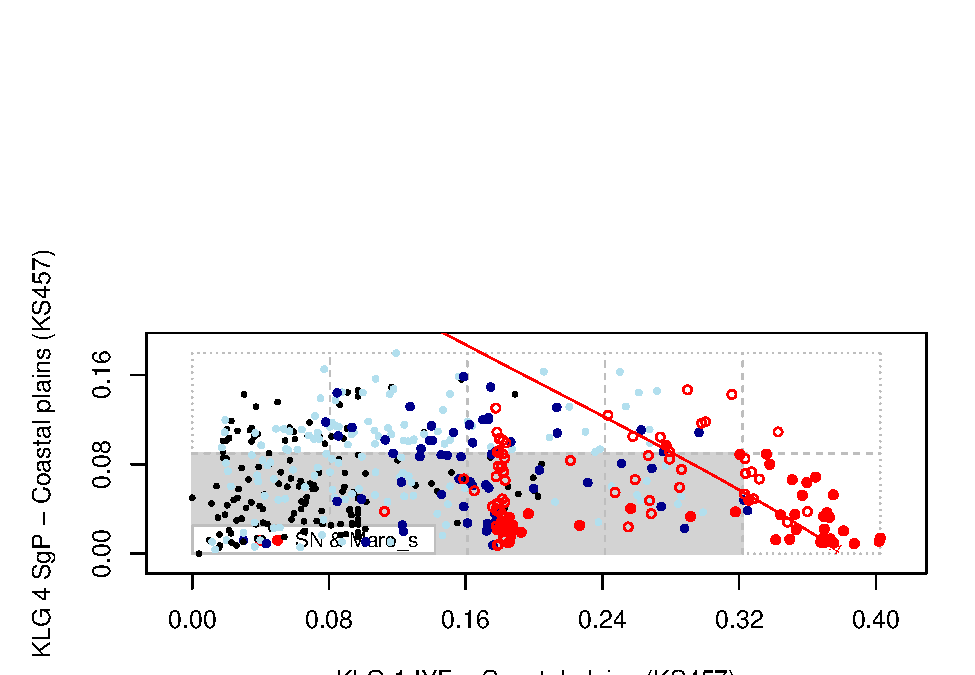
\includegraphics{Landscape_analysis_example_4_files/figure-latex/unnamed-chunk-51-1.pdf}

\begin{Shaded}
\begin{Highlighting}[]
\CommentTok{###}

\CommentTok{#Fig. 5. 1 IyK mot 4 SkP; SN som symboler og isolinjer for Arbla_a}

\CommentTok{#sONV'er som skal plottes mot hverandre}
\NormalTok{s1 <-}\StringTok{ }\NormalTok{sONV_IyK}
\NormalTok{s2 <-}\StringTok{ }\NormalTok{sONV_SkP}

\CommentTok{#Finner koordinatene for hj?rner i det 'plotteomr?det' med koordinater (x1, x2, y1, y2) som gir}
\CommentTok{#like enheter p? begge akser. Vi holder x1, x2 og y1 faste og bestemmer y2 slik at (x2-x1)/(y2-y1) i plt=c(x1,x2,y1,y2)}
\CommentTok{#blir lik max(s1)/max(s2)}
\CommentTok{#Det krever at y2 = [(x2-x1)*max(s2) + y1*max(s1)]/max(s1) }
\CommentTok{#Setter vi x1, x2 og y1 konstante, f?r vi:}
\NormalTok{y2 <-}\StringTok{ }\NormalTok{(}\FloatTok{0.8}\OperatorTok{*}\KeywordTok{max}\NormalTok{(s2)}\OperatorTok{+}\FloatTok{0.15}\OperatorTok{*}\KeywordTok{max}\NormalTok{(s1))}\OperatorTok{/}\KeywordTok{max}\NormalTok{(s1)}
\NormalTok{y2}
\end{Highlighting}
\end{Shaded}

\begin{verbatim}
## [1] 0.4929707
\end{verbatim}

\begin{Shaded}
\begin{Highlighting}[]
\KeywordTok{par}\NormalTok{(}\DataTypeTok{plt=}\KeywordTok{c}\NormalTok{(}\FloatTok{0.15}\NormalTok{, }\FloatTok{0.95}\NormalTok{, }\FloatTok{0.15}\NormalTok{, y2))}
\KeywordTok{plot}\NormalTok{(s1,s2,}\DataTypeTok{xlab=}\StringTok{"KLG 1 IYF - Coastal plains (KS457)"}\NormalTok{,}\DataTypeTok{ylab=}\StringTok{"KLG 4 SkP - Coastal plains (KS457)"}\NormalTok{,}\DataTypeTok{xlim=}\KeywordTok{c}\NormalTok{(}\OperatorTok{-}\FloatTok{0.01}\NormalTok{,}\KeywordTok{max}\NormalTok{(s1)}\OperatorTok{+}\FloatTok{0.01}\NormalTok{),}\DataTypeTok{ylim=}\KeywordTok{c}\NormalTok{(}\OperatorTok{-}\FloatTok{0.01}\NormalTok{,}\KeywordTok{max}\NormalTok{(s2)}\OperatorTok{+}\FloatTok{0.01}\NormalTok{),}\DataTypeTok{xaxp=}\KeywordTok{c}\NormalTok{(}\DecValTok{0}\NormalTok{,}\FloatTok{0.4}\NormalTok{,}\DecValTok{5}\NormalTok{),}\DataTypeTok{yaxp=}\KeywordTok{c}\NormalTok{(}\DecValTok{0}\NormalTok{,}\FloatTok{0.4}\NormalTok{,}\DecValTok{5}\NormalTok{),}\DataTypeTok{type=}\StringTok{"n"}\NormalTok{) }\CommentTok{#Grunnlag for plotting av symboler etc.}
\KeywordTok{lines}\NormalTok{(}\KeywordTok{c}\NormalTok{(}\DecValTok{0}\NormalTok{,}\KeywordTok{max}\NormalTok{(s1)),}\KeywordTok{c}\NormalTok{(}\KeywordTok{max}\NormalTok{(s2),}\KeywordTok{max}\NormalTok{(s2)),}\DataTypeTok{lty=}\DecValTok{3}\NormalTok{,}\DataTypeTok{col=}\DecValTok{8}\NormalTok{)}
\KeywordTok{lines}\NormalTok{(}\KeywordTok{c}\NormalTok{(}\DecValTok{0}\NormalTok{,}\KeywordTok{max}\NormalTok{(s1)),}\KeywordTok{c}\NormalTok{(}\DecValTok{0}\NormalTok{,}\DecValTok{0}\NormalTok{),}\DataTypeTok{lty=}\DecValTok{3}\NormalTok{,}\DataTypeTok{col=}\DecValTok{8}\NormalTok{)}
\KeywordTok{lines}\NormalTok{(}\KeywordTok{c}\NormalTok{(}\DecValTok{0}\NormalTok{,}\DecValTok{0}\NormalTok{),}\KeywordTok{c}\NormalTok{(}\DecValTok{0}\NormalTok{,}\KeywordTok{max}\NormalTok{(s2)),}\DataTypeTok{lty=}\DecValTok{3}\NormalTok{,}\DataTypeTok{col=}\DecValTok{8}\NormalTok{)}
\KeywordTok{lines}\NormalTok{(}\KeywordTok{c}\NormalTok{(}\KeywordTok{max}\NormalTok{(s1),}\KeywordTok{max}\NormalTok{(s1)),}\KeywordTok{c}\NormalTok{(}\DecValTok{0}\NormalTok{,}\KeywordTok{max}\NormalTok{(s2)),}\DataTypeTok{lty=}\DecValTok{3}\NormalTok{,}\DataTypeTok{col=}\DecValTok{8}\NormalTok{)}

\KeywordTok{polygon}\NormalTok{(}\KeywordTok{c}\NormalTok{(}\DecValTok{4}\OperatorTok{*}\KeywordTok{max}\NormalTok{(s1)}\OperatorTok{/}\DecValTok{5}\NormalTok{,}\DecValTok{4}\OperatorTok{*}\KeywordTok{max}\NormalTok{(s1)}\OperatorTok{/}\DecValTok{5}\NormalTok{,}\KeywordTok{max}\NormalTok{(s1),}\KeywordTok{max}\NormalTok{(s1)),}\KeywordTok{c}\NormalTok{(}\FloatTok{0.025}\NormalTok{,}\KeywordTok{max}\NormalTok{(s2),}\KeywordTok{max}\NormalTok{(s2),}\FloatTok{0.025}\NormalTok{),}\DataTypeTok{col=}\StringTok{"lightgray"}\NormalTok{)}
\KeywordTok{polygon}\NormalTok{(}\KeywordTok{c}\NormalTok{(}\DecValTok{4}\OperatorTok{*}\KeywordTok{max}\NormalTok{(s1)}\OperatorTok{/}\DecValTok{5}\NormalTok{,}\DecValTok{4}\OperatorTok{*}\KeywordTok{max}\NormalTok{(s1)}\OperatorTok{/}\DecValTok{5}\NormalTok{,}\KeywordTok{max}\NormalTok{(s1),}\KeywordTok{max}\NormalTok{(s1)),}\KeywordTok{c}\NormalTok{(}\FloatTok{0.025}\NormalTok{,}\KeywordTok{max}\NormalTok{(s2),}\KeywordTok{max}\NormalTok{(s2),}\FloatTok{0.025}\NormalTok{),}\DataTypeTok{col=}\StringTok{"lightgray"}\NormalTok{,}\DataTypeTok{density=}\DecValTok{10}\NormalTok{) }\CommentTok{#legger egentlig et skr?tt raster opp?, og fjerner streken rundt}

\KeywordTok{polygon}\NormalTok{(}\KeywordTok{c}\NormalTok{(}\KeywordTok{max}\NormalTok{(s1)}\OperatorTok{-}\FloatTok{0.142}\NormalTok{,}\KeywordTok{max}\NormalTok{(s1)}\OperatorTok{-}\FloatTok{0.142}\NormalTok{,}\DecValTok{4}\OperatorTok{*}\KeywordTok{max}\NormalTok{(s1)}\OperatorTok{/}\DecValTok{5}\NormalTok{,}\DecValTok{4}\OperatorTok{*}\KeywordTok{max}\NormalTok{(s1)}\OperatorTok{/}\DecValTok{5}\NormalTok{),}\KeywordTok{c}\NormalTok{(}\FloatTok{0.025}\NormalTok{,}\KeywordTok{max}\NormalTok{(s2)}\OperatorTok{/}\DecValTok{2}\NormalTok{,}\KeywordTok{max}\NormalTok{(s2)}\OperatorTok{/}\DecValTok{2}\NormalTok{,}\FloatTok{0.025}\NormalTok{),}\DataTypeTok{col=}\StringTok{"lightgray"}\NormalTok{)}
\KeywordTok{polygon}\NormalTok{(}\KeywordTok{c}\NormalTok{(}\KeywordTok{max}\NormalTok{(s1)}\OperatorTok{-}\FloatTok{0.142}\NormalTok{,}\KeywordTok{max}\NormalTok{(s1)}\OperatorTok{-}\FloatTok{0.142}\NormalTok{,}\DecValTok{4}\OperatorTok{*}\KeywordTok{max}\NormalTok{(s1)}\OperatorTok{/}\DecValTok{5}\NormalTok{,}\DecValTok{4}\OperatorTok{*}\KeywordTok{max}\NormalTok{(s1)}\OperatorTok{/}\DecValTok{5}\NormalTok{),}\KeywordTok{c}\NormalTok{(}\FloatTok{0.025}\NormalTok{,}\KeywordTok{max}\NormalTok{(s2)}\OperatorTok{/}\DecValTok{2}\NormalTok{,}\KeywordTok{max}\NormalTok{(s2)}\OperatorTok{/}\DecValTok{2}\NormalTok{,}\FloatTok{0.025}\NormalTok{),}\DataTypeTok{col=}\StringTok{"lightgray"}\NormalTok{,}\DataTypeTok{density=}\DecValTok{10}\NormalTok{) }\CommentTok{#legger egentlig et skr?tt raster opp?, og fjerner streken rundt}

\KeywordTok{polygon}\NormalTok{(}\KeywordTok{c}\NormalTok{(}\DecValTok{3}\OperatorTok{*}\KeywordTok{max}\NormalTok{(s1)}\OperatorTok{/}\DecValTok{5}\NormalTok{,}\DecValTok{3}\OperatorTok{*}\KeywordTok{max}\NormalTok{(s1)}\OperatorTok{/}\DecValTok{5}\NormalTok{,}\KeywordTok{max}\NormalTok{(s1)}\OperatorTok{-}\FloatTok{0.142}\NormalTok{,}\KeywordTok{max}\NormalTok{(s1)}\OperatorTok{-}\FloatTok{0.142}\NormalTok{),}\KeywordTok{c}\NormalTok{(}\DecValTok{0}\NormalTok{,}\KeywordTok{max}\NormalTok{(s2)}\OperatorTok{/}\DecValTok{2}\NormalTok{,}\KeywordTok{max}\NormalTok{(s2)}\OperatorTok{/}\DecValTok{2}\NormalTok{,}\DecValTok{0}\NormalTok{),}\DataTypeTok{col=}\StringTok{"lightgray"}\NormalTok{)}
\KeywordTok{polygon}\NormalTok{(}\KeywordTok{c}\NormalTok{(}\DecValTok{3}\OperatorTok{*}\KeywordTok{max}\NormalTok{(s1)}\OperatorTok{/}\DecValTok{5}\NormalTok{,}\DecValTok{3}\OperatorTok{*}\KeywordTok{max}\NormalTok{(s1)}\OperatorTok{/}\DecValTok{5}\NormalTok{,}\KeywordTok{max}\NormalTok{(s1)}\OperatorTok{-}\FloatTok{0.142}\NormalTok{,}\KeywordTok{max}\NormalTok{(s1)}\OperatorTok{-}\FloatTok{0.142}\NormalTok{),}\KeywordTok{c}\NormalTok{(}\DecValTok{0}\NormalTok{,}\KeywordTok{max}\NormalTok{(s2)}\OperatorTok{/}\DecValTok{2}\NormalTok{,}\KeywordTok{max}\NormalTok{(s2)}\OperatorTok{/}\DecValTok{2}\NormalTok{,}\DecValTok{0}\NormalTok{),}\DataTypeTok{col=}\StringTok{"lightgray"}\NormalTok{,}\DataTypeTok{density=}\DecValTok{10}\NormalTok{) }\CommentTok{#legger egentlig et skr?tt raster opp?, og fjerner streken rundt}

\KeywordTok{lines}\NormalTok{(}\KeywordTok{c}\NormalTok{(}\DecValTok{0}\NormalTok{,}\KeywordTok{max}\NormalTok{(s1)),}\KeywordTok{c}\NormalTok{(}\KeywordTok{max}\NormalTok{(s2)}\OperatorTok{/}\DecValTok{2}\NormalTok{,}\KeywordTok{max}\NormalTok{(s2)}\OperatorTok{/}\DecValTok{2}\NormalTok{),}\DataTypeTok{lty=}\DecValTok{2}\NormalTok{,}\DataTypeTok{col=}\DecValTok{8}\NormalTok{)}
\KeywordTok{lines}\NormalTok{(}\KeywordTok{c}\NormalTok{(}\FloatTok{0.2}\OperatorTok{*}\KeywordTok{max}\NormalTok{(s1),}\FloatTok{0.2}\OperatorTok{*}\KeywordTok{max}\NormalTok{(s1)),}\KeywordTok{c}\NormalTok{(}\DecValTok{0}\NormalTok{,}\KeywordTok{max}\NormalTok{(s2)),}\DataTypeTok{lty=}\DecValTok{2}\NormalTok{,}\DataTypeTok{col=}\DecValTok{8}\NormalTok{)}
\KeywordTok{lines}\NormalTok{(}\KeywordTok{c}\NormalTok{(}\FloatTok{0.4}\OperatorTok{*}\KeywordTok{max}\NormalTok{(s1),}\FloatTok{0.4}\OperatorTok{*}\KeywordTok{max}\NormalTok{(s1)),}\KeywordTok{c}\NormalTok{(}\DecValTok{0}\NormalTok{,}\KeywordTok{max}\NormalTok{(s2)),}\DataTypeTok{lty=}\DecValTok{2}\NormalTok{,}\DataTypeTok{col=}\DecValTok{8}\NormalTok{)}
\KeywordTok{lines}\NormalTok{(}\KeywordTok{c}\NormalTok{(}\FloatTok{0.6}\OperatorTok{*}\KeywordTok{max}\NormalTok{(s1),}\FloatTok{0.6}\OperatorTok{*}\KeywordTok{max}\NormalTok{(s1)),}\KeywordTok{c}\NormalTok{(}\DecValTok{0}\NormalTok{,}\KeywordTok{max}\NormalTok{(s2)),}\DataTypeTok{lty=}\DecValTok{2}\NormalTok{,}\DataTypeTok{col=}\DecValTok{8}\NormalTok{)}
\KeywordTok{lines}\NormalTok{(}\KeywordTok{c}\NormalTok{(}\FloatTok{0.8}\OperatorTok{*}\KeywordTok{max}\NormalTok{(s1),}\FloatTok{0.8}\OperatorTok{*}\KeywordTok{max}\NormalTok{(s1)),}\KeywordTok{c}\NormalTok{(}\DecValTok{0}\NormalTok{,}\KeywordTok{max}\NormalTok{(s2)}\OperatorTok{-}\FloatTok{0.025}\NormalTok{),}\DataTypeTok{lty=}\DecValTok{2}\NormalTok{,}\DataTypeTok{col=}\DecValTok{8}\NormalTok{)}

\KeywordTok{lines}\NormalTok{(}\KeywordTok{c}\NormalTok{(}\KeywordTok{max}\NormalTok{(s1)}\OperatorTok{-}\FloatTok{0.142}\NormalTok{,}\KeywordTok{max}\NormalTok{(s1)),}\KeywordTok{c}\NormalTok{(}\DecValTok{0}\NormalTok{,}\DecValTok{0}\NormalTok{),}\DataTypeTok{col=}\DecValTok{8}\NormalTok{)}
\KeywordTok{lines}\NormalTok{(}\KeywordTok{c}\NormalTok{(}\KeywordTok{max}\NormalTok{(s1)}\OperatorTok{-}\FloatTok{0.142}\NormalTok{,}\KeywordTok{max}\NormalTok{(s1)),}\KeywordTok{c}\NormalTok{(}\FloatTok{0.025}\NormalTok{,}\FloatTok{0.025}\NormalTok{),}\DataTypeTok{col=}\DecValTok{8}\NormalTok{)}
\KeywordTok{lines}\NormalTok{(}\KeywordTok{c}\NormalTok{(}\KeywordTok{max}\NormalTok{(s1)}\OperatorTok{-}\FloatTok{0.142}\NormalTok{,}\KeywordTok{max}\NormalTok{(s1)}\OperatorTok{-}\FloatTok{0.142}\NormalTok{),}\KeywordTok{c}\NormalTok{(}\DecValTok{0}\NormalTok{,}\FloatTok{0.025}\NormalTok{),}\DataTypeTok{col=}\DecValTok{8}\NormalTok{)}
\KeywordTok{lines}\NormalTok{(}\KeywordTok{c}\NormalTok{(}\KeywordTok{max}\NormalTok{(s1),}\KeywordTok{max}\NormalTok{(s1)),}\KeywordTok{c}\NormalTok{(}\DecValTok{0}\NormalTok{,}\FloatTok{0.025}\NormalTok{),}\DataTypeTok{col=}\DecValTok{8}\NormalTok{)}

\KeywordTok{points}\NormalTok{(}\KeywordTok{max}\NormalTok{(s1)}\OperatorTok{-}\FloatTok{0.142+0.01}\NormalTok{,}\FloatTok{0.012}\NormalTok{,}\DataTypeTok{pch=}\DecValTok{16}\NormalTok{,}\DataTypeTok{cex=}\FloatTok{0.5}\NormalTok{,}\DataTypeTok{col=}\StringTok{"black"}\NormalTok{)}
\KeywordTok{points}\NormalTok{(}\KeywordTok{max}\NormalTok{(s1)}\OperatorTok{-}\FloatTok{0.142+0.02}\NormalTok{,}\FloatTok{0.012}\NormalTok{,}\DataTypeTok{pch=}\DecValTok{16}\NormalTok{,}\DataTypeTok{cex=}\FloatTok{0.6}\NormalTok{,}\DataTypeTok{col=}\StringTok{"lightblue2"}\NormalTok{)}
\KeywordTok{points}\NormalTok{(}\KeywordTok{max}\NormalTok{(s1)}\OperatorTok{-}\FloatTok{0.142+0.03}\NormalTok{,}\FloatTok{0.012}\NormalTok{,}\DataTypeTok{pch=}\DecValTok{16}\NormalTok{,}\DataTypeTok{cex=}\FloatTok{0.75}\NormalTok{,}\DataTypeTok{col=}\StringTok{"darkblue"}\NormalTok{)}
\KeywordTok{points}\NormalTok{(}\KeywordTok{max}\NormalTok{(s1)}\OperatorTok{-}\FloatTok{0.142+0.04}\NormalTok{,}\FloatTok{0.012}\NormalTok{,}\DataTypeTok{pch=}\DecValTok{1}\NormalTok{,}\DataTypeTok{cex=}\FloatTok{0.75}\NormalTok{,}\DataTypeTok{col=}\StringTok{"red"}\NormalTok{)}
\KeywordTok{points}\NormalTok{(}\KeywordTok{max}\NormalTok{(s1)}\OperatorTok{-}\FloatTok{0.142+0.05}\NormalTok{,}\FloatTok{0.012}\NormalTok{,}\DataTypeTok{pch=}\DecValTok{16}\NormalTok{,}\DataTypeTok{cex=}\FloatTok{0.9}\NormalTok{,}\DataTypeTok{col=}\StringTok{"red"}\NormalTok{)}

\KeywordTok{text}\NormalTok{(}\KeywordTok{max}\NormalTok{(s1)}\OperatorTok{-}\FloatTok{0.142+0.06}\NormalTok{,}\FloatTok{0.012}\NormalTok{,}\StringTok{"SN & Arbla_a"}\NormalTok{,}\DataTypeTok{adj=}\DecValTok{0}\NormalTok{,}\DataTypeTok{cex=}\FloatTok{0.8}\NormalTok{)}
\KeywordTok{points}\NormalTok{(s1[SN}\OperatorTok{==}\DecValTok{1}\NormalTok{],s2[SN}\OperatorTok{==}\DecValTok{1}\NormalTok{],}\DataTypeTok{pch=}\DecValTok{16}\NormalTok{,}\DataTypeTok{cex=}\FloatTok{0.5}\NormalTok{,}\DataTypeTok{col=}\DecValTok{1}\NormalTok{)}
\KeywordTok{points}\NormalTok{(s1[SN}\OperatorTok{==}\DecValTok{2}\NormalTok{],s2[SN}\OperatorTok{==}\DecValTok{2}\NormalTok{],}\DataTypeTok{pch=}\DecValTok{16}\NormalTok{,}\DataTypeTok{cex=}\FloatTok{0.6}\NormalTok{,}\DataTypeTok{col=}\StringTok{"lightblue2"}\NormalTok{)}
\KeywordTok{points}\NormalTok{(s1[SN}\OperatorTok{==}\DecValTok{3}\NormalTok{],s2[SN}\OperatorTok{==}\DecValTok{3}\NormalTok{],}\DataTypeTok{pch=}\DecValTok{16}\NormalTok{,}\DataTypeTok{cex=}\FloatTok{0.75}\NormalTok{,}\DataTypeTok{col=}\StringTok{"darkblue"}\NormalTok{)}
\KeywordTok{points}\NormalTok{(s1[SN}\OperatorTok{==}\DecValTok{4}\NormalTok{],s2[SN}\OperatorTok{==}\DecValTok{4}\NormalTok{],}\DataTypeTok{pch=}\DecValTok{1}\NormalTok{,}\DataTypeTok{cex=}\FloatTok{0.75}\NormalTok{,}\DataTypeTok{col=}\StringTok{"red"}\NormalTok{)}
\KeywordTok{points}\NormalTok{(s1[SN}\OperatorTok{==}\DecValTok{5}\NormalTok{],s2[SN}\OperatorTok{==}\DecValTok{5}\NormalTok{],}\DataTypeTok{pch=}\DecValTok{16}\NormalTok{,}\DataTypeTok{cex=}\FloatTok{0.9}\NormalTok{,}\DataTypeTok{col=}\StringTok{"red"}\NormalTok{)}

\NormalTok{os <-}\StringTok{ }\KeywordTok{ordisurf}\NormalTok{(snv[,}\KeywordTok{c}\NormalTok{(}\DecValTok{1}\NormalTok{,}\DecValTok{4}\NormalTok{)],Arbla_a,}\DataTypeTok{display=}\StringTok{"sites"}\NormalTok{,}\DataTypeTok{levels=}\KeywordTok{c}\NormalTok{(}\FloatTok{0.1}\NormalTok{,}\FloatTok{0.2}\NormalTok{,}\FloatTok{0.3}\NormalTok{,}\FloatTok{0.4}\NormalTok{,}\FloatTok{0.5}\NormalTok{,}\FloatTok{0.6}\NormalTok{,}\FloatTok{0.7}\NormalTok{), }\DataTypeTok{col=}\StringTok{"red"}\NormalTok{,}\DataTypeTok{add=}\NormalTok{T) }\CommentTok{#inkluderer plotting p? eksisterende ordinasjonsdiagram}
\end{Highlighting}
\end{Shaded}

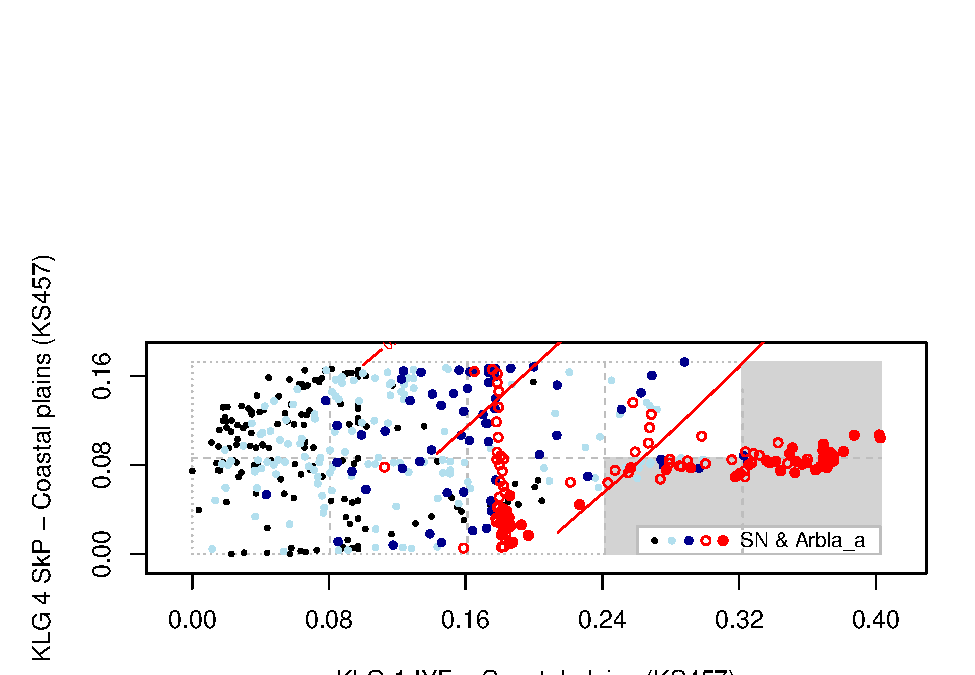
\includegraphics{Landscape_analysis_example_4_files/figure-latex/unnamed-chunk-52-1.pdf}

\begin{Shaded}
\begin{Highlighting}[]
\CommentTok{###}

\CommentTok{#Fig. 6. 1 IyK mot 6 OI; OI som symboler og isolinjer for Gab_a}

\CommentTok{#sONV'er som skal plottes mot hverandre}
\NormalTok{s1 <-}\StringTok{ }\NormalTok{sONV_IyK}
\NormalTok{s2 <-}\StringTok{ }\NormalTok{sONV_OI}

\CommentTok{#Finner koordinatene for hj?rner i det 'plotteomr?det' med koordinater (x1, x2, y1, y2) som gir}
\CommentTok{#like enheter p? begge akser. Vi holder x1, x2 og y1 faste og bestemmer y2 slik at (x2-x1)/(y2-y1) i plt=c(x1,x2,y1,y2)}
\CommentTok{#blir lik max(s1)/max(s2)}
\CommentTok{#Det krever at y2 = [(x2-x1)*max(s2) + y1*max(s1)]/max(s1) }
\CommentTok{#Setter vi x1, x2 og y1 konstante, f?r vi:}
\NormalTok{y2 <-}\StringTok{ }\NormalTok{(}\FloatTok{0.8}\OperatorTok{*}\KeywordTok{max}\NormalTok{(s2)}\OperatorTok{+}\FloatTok{0.15}\OperatorTok{*}\KeywordTok{max}\NormalTok{(s1))}\OperatorTok{/}\KeywordTok{max}\NormalTok{(s1)}
\NormalTok{y2}
\end{Highlighting}
\end{Shaded}

\begin{verbatim}
## [1] 0.4170641
\end{verbatim}

\begin{Shaded}
\begin{Highlighting}[]
\CommentTok{#Plotter OI-klasser p? figuren, og legger p? isolinjer for Gab_a}
\KeywordTok{par}\NormalTok{(}\DataTypeTok{plt=}\KeywordTok{c}\NormalTok{(}\FloatTok{0.15}\NormalTok{, }\FloatTok{0.95}\NormalTok{, }\FloatTok{0.15}\NormalTok{, y2))}
\KeywordTok{plot}\NormalTok{(s1,s2,}\DataTypeTok{xlab=}\StringTok{"KLG 1 IYF - Coastal plains (KS457)"}\NormalTok{,}\DataTypeTok{ylab=}\StringTok{"KLG 6 Gab_a - Coastal plains (KS457)"}\NormalTok{,}\DataTypeTok{xlim=}\KeywordTok{c}\NormalTok{(}\OperatorTok{-}\FloatTok{0.01}\NormalTok{,}\KeywordTok{max}\NormalTok{(s1)}\OperatorTok{+}\FloatTok{0.01}\NormalTok{),}\DataTypeTok{ylim=}\KeywordTok{c}\NormalTok{(}\OperatorTok{-}\FloatTok{0.01}\NormalTok{,}\KeywordTok{max}\NormalTok{(s2)}\OperatorTok{+}\FloatTok{0.01}\NormalTok{),}\DataTypeTok{xaxp=}\KeywordTok{c}\NormalTok{(}\DecValTok{0}\NormalTok{,}\FloatTok{0.4}\NormalTok{,}\DecValTok{5}\NormalTok{),}\DataTypeTok{yaxp=}\KeywordTok{c}\NormalTok{(}\DecValTok{0}\NormalTok{,}\FloatTok{0.4}\NormalTok{,}\DecValTok{5}\NormalTok{),}\DataTypeTok{type=}\StringTok{"n"}\NormalTok{) }\CommentTok{#Grunnlag for plotting av symboler etc.}
\KeywordTok{lines}\NormalTok{(}\KeywordTok{c}\NormalTok{(}\DecValTok{0}\NormalTok{,}\KeywordTok{max}\NormalTok{(s1)),}\KeywordTok{c}\NormalTok{(}\KeywordTok{max}\NormalTok{(s2),}\KeywordTok{max}\NormalTok{(s2)),}\DataTypeTok{lty=}\DecValTok{3}\NormalTok{,}\DataTypeTok{col=}\DecValTok{8}\NormalTok{)}
\KeywordTok{lines}\NormalTok{(}\KeywordTok{c}\NormalTok{(}\DecValTok{0}\NormalTok{,}\KeywordTok{max}\NormalTok{(s1)),}\KeywordTok{c}\NormalTok{(}\DecValTok{0}\NormalTok{,}\DecValTok{0}\NormalTok{),}\DataTypeTok{lty=}\DecValTok{3}\NormalTok{,}\DataTypeTok{col=}\DecValTok{8}\NormalTok{)}
\KeywordTok{lines}\NormalTok{(}\KeywordTok{c}\NormalTok{(}\DecValTok{0}\NormalTok{,}\DecValTok{0}\NormalTok{),}\KeywordTok{c}\NormalTok{(}\DecValTok{0}\NormalTok{,}\KeywordTok{max}\NormalTok{(s2)),}\DataTypeTok{lty=}\DecValTok{3}\NormalTok{,}\DataTypeTok{col=}\DecValTok{8}\NormalTok{)}
\KeywordTok{lines}\NormalTok{(}\KeywordTok{c}\NormalTok{(}\KeywordTok{max}\NormalTok{(s1),}\KeywordTok{max}\NormalTok{(s1)),}\KeywordTok{c}\NormalTok{(}\DecValTok{0}\NormalTok{,}\KeywordTok{max}\NormalTok{(s2)),}\DataTypeTok{lty=}\DecValTok{3}\NormalTok{,}\DataTypeTok{col=}\DecValTok{8}\NormalTok{)}

\KeywordTok{lines}\NormalTok{(}\KeywordTok{c}\NormalTok{(}\DecValTok{0}\NormalTok{,}\KeywordTok{max}\NormalTok{(s1)),}\KeywordTok{c}\NormalTok{(}\KeywordTok{max}\NormalTok{(s2)}\OperatorTok{/}\DecValTok{2}\NormalTok{,}\KeywordTok{max}\NormalTok{(s2)}\OperatorTok{/}\DecValTok{2}\NormalTok{),}\DataTypeTok{lty=}\DecValTok{2}\NormalTok{,}\DataTypeTok{col=}\DecValTok{8}\NormalTok{)}
\KeywordTok{lines}\NormalTok{(}\KeywordTok{c}\NormalTok{(}\FloatTok{0.2}\OperatorTok{*}\KeywordTok{max}\NormalTok{(s1),}\FloatTok{0.2}\OperatorTok{*}\KeywordTok{max}\NormalTok{(s1)),}\KeywordTok{c}\NormalTok{(}\DecValTok{0}\NormalTok{,}\KeywordTok{max}\NormalTok{(s2)}\OperatorTok{-}\FloatTok{0.025}\NormalTok{),}\DataTypeTok{lty=}\DecValTok{2}\NormalTok{,}\DataTypeTok{col=}\DecValTok{8}\NormalTok{)}
\KeywordTok{lines}\NormalTok{(}\KeywordTok{c}\NormalTok{(}\FloatTok{0.4}\OperatorTok{*}\KeywordTok{max}\NormalTok{(s1),}\FloatTok{0.4}\OperatorTok{*}\KeywordTok{max}\NormalTok{(s1)),}\KeywordTok{c}\NormalTok{(}\DecValTok{0}\NormalTok{,}\KeywordTok{max}\NormalTok{(s2)),}\DataTypeTok{lty=}\DecValTok{2}\NormalTok{,}\DataTypeTok{col=}\DecValTok{8}\NormalTok{)}
\KeywordTok{lines}\NormalTok{(}\KeywordTok{c}\NormalTok{(}\FloatTok{0.6}\OperatorTok{*}\KeywordTok{max}\NormalTok{(s1),}\FloatTok{0.6}\OperatorTok{*}\KeywordTok{max}\NormalTok{(s1)),}\KeywordTok{c}\NormalTok{(}\DecValTok{0}\NormalTok{,}\KeywordTok{max}\NormalTok{(s2)),}\DataTypeTok{lty=}\DecValTok{2}\NormalTok{,}\DataTypeTok{col=}\DecValTok{8}\NormalTok{)}
\KeywordTok{lines}\NormalTok{(}\KeywordTok{c}\NormalTok{(}\FloatTok{0.8}\OperatorTok{*}\KeywordTok{max}\NormalTok{(s1),}\FloatTok{0.8}\OperatorTok{*}\KeywordTok{max}\NormalTok{(s1)),}\KeywordTok{c}\NormalTok{(}\DecValTok{0}\NormalTok{,}\KeywordTok{max}\NormalTok{(s2)),}\DataTypeTok{lty=}\DecValTok{2}\NormalTok{,}\DataTypeTok{col=}\DecValTok{8}\NormalTok{)}

\KeywordTok{lines}\NormalTok{(}\KeywordTok{c}\NormalTok{(}\DecValTok{0}\NormalTok{,}\FloatTok{0.142}\NormalTok{),}\KeywordTok{c}\NormalTok{(}\DecValTok{0}\NormalTok{,}\DecValTok{0}\NormalTok{),}\DataTypeTok{col=}\DecValTok{8}\NormalTok{)}
\KeywordTok{lines}\NormalTok{(}\KeywordTok{c}\NormalTok{(}\DecValTok{0}\NormalTok{,}\FloatTok{0.142}\NormalTok{),}\KeywordTok{c}\NormalTok{(}\FloatTok{0.025}\NormalTok{,}\FloatTok{0.025}\NormalTok{),}\DataTypeTok{col=}\DecValTok{8}\NormalTok{)}
\KeywordTok{lines}\NormalTok{(}\KeywordTok{c}\NormalTok{(}\FloatTok{0.142}\NormalTok{,}\FloatTok{0.142}\NormalTok{),}\KeywordTok{c}\NormalTok{(}\DecValTok{0}\NormalTok{,}\FloatTok{0.025}\NormalTok{),}\DataTypeTok{col=}\DecValTok{8}\NormalTok{)}
\KeywordTok{lines}\NormalTok{(}\KeywordTok{c}\NormalTok{(}\DecValTok{0}\NormalTok{,}\DecValTok{0}\NormalTok{),}\KeywordTok{c}\NormalTok{(}\DecValTok{0}\NormalTok{,}\FloatTok{0.025}\NormalTok{),}\DataTypeTok{col=}\DecValTok{8}\NormalTok{)}

\KeywordTok{points}\NormalTok{(}\FloatTok{0.01}\NormalTok{,}\FloatTok{0.012}\NormalTok{,}\DataTypeTok{pch=}\DecValTok{1}\NormalTok{,}\DataTypeTok{cex=}\FloatTok{0.6}\NormalTok{,}\DataTypeTok{col=}\StringTok{"lightblue3"}\NormalTok{)}
\KeywordTok{points}\NormalTok{(}\FloatTok{0.02}\NormalTok{,}\FloatTok{0.012}\NormalTok{,}\DataTypeTok{pch=}\DecValTok{16}\NormalTok{,}\DataTypeTok{cex=}\FloatTok{0.6}\NormalTok{,}\DataTypeTok{col=}\StringTok{"lightblue3"}\NormalTok{)}
\KeywordTok{points}\NormalTok{(}\FloatTok{0.03}\NormalTok{,}\FloatTok{0.012}\NormalTok{,}\DataTypeTok{pch=}\DecValTok{1}\NormalTok{,}\DataTypeTok{cex=}\FloatTok{0.75}\NormalTok{,}\DataTypeTok{col=}\StringTok{"lightblue4"}\NormalTok{)}
\KeywordTok{points}\NormalTok{(}\FloatTok{0.04}\NormalTok{,}\FloatTok{0.012}\NormalTok{,}\DataTypeTok{pch=}\DecValTok{16}\NormalTok{,}\DataTypeTok{cex=}\FloatTok{0.75}\NormalTok{,}\DataTypeTok{col=}\StringTok{"lightblue4"}\NormalTok{)}
\KeywordTok{points}\NormalTok{(}\FloatTok{0.05}\NormalTok{,}\FloatTok{0.012}\NormalTok{,}\DataTypeTok{pch=}\DecValTok{1}\NormalTok{,}\DataTypeTok{cex=}\FloatTok{0.9}\NormalTok{,}\DataTypeTok{col=}\StringTok{"red"}\NormalTok{)}
\KeywordTok{points}\NormalTok{(}\FloatTok{0.06}\NormalTok{,}\FloatTok{0.012}\NormalTok{,}\DataTypeTok{pch=}\DecValTok{16}\NormalTok{,}\DataTypeTok{cex=}\FloatTok{0.9}\NormalTok{,}\DataTypeTok{col=}\StringTok{"red"}\NormalTok{)}

\KeywordTok{text}\NormalTok{(}\FloatTok{0.07}\NormalTok{,}\FloatTok{0.012}\NormalTok{,}\StringTok{"OI & Gab_a"}\NormalTok{,}\DataTypeTok{adj=}\DecValTok{0}\NormalTok{,}\DataTypeTok{cex=}\FloatTok{0.8}\NormalTok{)}
\KeywordTok{points}\NormalTok{(s1[OI}\OperatorTok{==}\DecValTok{1}\NormalTok{],s2[OI}\OperatorTok{==}\DecValTok{1}\NormalTok{],}\DataTypeTok{pch=}\DecValTok{1}\NormalTok{,}\DataTypeTok{cex=}\FloatTok{0.6}\NormalTok{,}\DataTypeTok{col=}\StringTok{"lightblue3"}\NormalTok{)}
\KeywordTok{points}\NormalTok{(s1[OI}\OperatorTok{==}\DecValTok{2}\NormalTok{],s2[OI}\OperatorTok{==}\DecValTok{2}\NormalTok{],}\DataTypeTok{pch=}\DecValTok{16}\NormalTok{,}\DataTypeTok{cex=}\FloatTok{0.6}\NormalTok{,}\DataTypeTok{col=}\StringTok{"lightblue3"}\NormalTok{)}
\KeywordTok{points}\NormalTok{(s1[OI}\OperatorTok{==}\DecValTok{3}\NormalTok{],s2[OI}\OperatorTok{==}\DecValTok{3}\NormalTok{],}\DataTypeTok{pch=}\DecValTok{1}\NormalTok{,}\DataTypeTok{cex=}\FloatTok{0.75}\NormalTok{,}\DataTypeTok{col=}\StringTok{"lightblue4"}\NormalTok{)}
\KeywordTok{points}\NormalTok{(s1[OI}\OperatorTok{==}\DecValTok{4}\NormalTok{],s2[OI}\OperatorTok{==}\DecValTok{4}\NormalTok{],}\DataTypeTok{pch=}\DecValTok{16}\NormalTok{,}\DataTypeTok{cex=}\FloatTok{0.75}\NormalTok{,}\DataTypeTok{col=}\StringTok{"lightblue4"}\NormalTok{)}
\KeywordTok{points}\NormalTok{(s1[OI}\OperatorTok{==}\DecValTok{5}\NormalTok{],s2[OI}\OperatorTok{==}\DecValTok{5}\NormalTok{],}\DataTypeTok{pch=}\DecValTok{1}\NormalTok{,}\DataTypeTok{cex=}\FloatTok{0.9}\NormalTok{,}\DataTypeTok{col=}\StringTok{"red"}\NormalTok{)}
\KeywordTok{points}\NormalTok{(s1[OI}\OperatorTok{==}\DecValTok{6}\NormalTok{],s2[OI}\OperatorTok{==}\DecValTok{6}\NormalTok{],}\DataTypeTok{pch=}\DecValTok{16}\NormalTok{,}\DataTypeTok{cex=}\FloatTok{0.9}\NormalTok{,}\DataTypeTok{col=}\StringTok{"red"}\NormalTok{)}

\NormalTok{os <-}\StringTok{ }\KeywordTok{ordisurf}\NormalTok{(snv[,}\KeywordTok{c}\NormalTok{(}\DecValTok{1}\NormalTok{,}\DecValTok{6}\NormalTok{)],Gab_a,}\DataTypeTok{display=}\StringTok{"sites"}\NormalTok{,}\DataTypeTok{levels=}\KeywordTok{c}\NormalTok{(}\FloatTok{0.1}\NormalTok{,}\FloatTok{0.2}\NormalTok{,}\FloatTok{0.4}\NormalTok{,}\FloatTok{0.6}\NormalTok{,}\FloatTok{0.8}\NormalTok{), }\DataTypeTok{col=}\StringTok{"red"}\NormalTok{,}\DataTypeTok{add=}\NormalTok{T) }\CommentTok{#inkluderer plotting p? eksisterende ordinasjonsdiagram}
\end{Highlighting}
\end{Shaded}

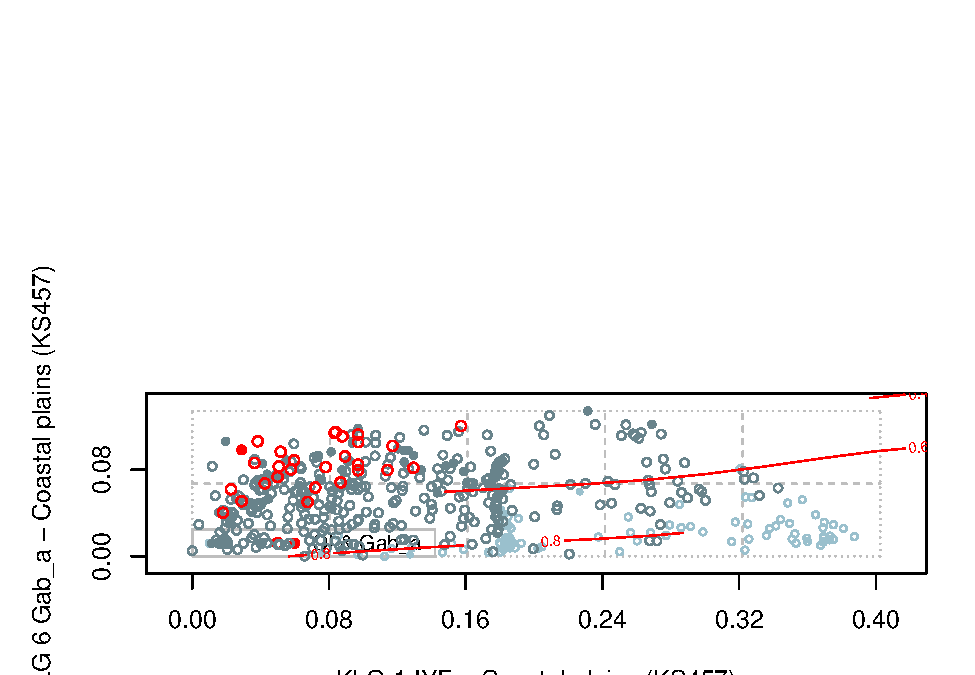
\includegraphics{Landscape_analysis_example_4_files/figure-latex/unnamed-chunk-53-1.pdf}

\begin{Shaded}
\begin{Highlighting}[]
\KeywordTok{library}\NormalTok{(goeveg)}
\end{Highlighting}
\end{Shaded}

\begin{verbatim}
## Welcome to the GoeVeg Package
\end{verbatim}

\begin{Shaded}
\begin{Highlighting}[]
\KeywordTok{library}\NormalTok{(vegan)}

\KeywordTok{palette}\NormalTok{(}\KeywordTok{c}\NormalTok{(}\StringTok{"#a6cee3"}\NormalTok{, }\StringTok{"#1f78b4"}\NormalTok{, }\StringTok{"#b2df8a"}\NormalTok{, }\StringTok{"#33a02c"}\NormalTok{, }\StringTok{"#fb9a99"}\NormalTok{, }\StringTok{"#e31a1c"}\NormalTok{, }
                    \StringTok{"#fdbf6f"}\NormalTok{, }\StringTok{"#ff7f00"}\NormalTok{, }\StringTok{"#cab2d6"}\NormalTok{, }\StringTok{"#6a3d9a"}\NormalTok{, }\StringTok{"#ffff99"}\NormalTok{, }\StringTok{"#b15928"}\NormalTok{))}
\CommentTok{#rgb( ramp(seq(0, 1, length = 5)), max = 255)}

\NormalTok{specresponse2 <-}\StringTok{ }\ControlFlowTok{function}\NormalTok{(species, var, main, xlab, }\DataTypeTok{model =} \StringTok{"auto"}\NormalTok{, }\DataTypeTok{method =} \StringTok{"env"}\NormalTok{, }\DataTypeTok{axis =} \DecValTok{1}\NormalTok{, }\DataTypeTok{points =} \OtherTok{FALSE}\NormalTok{, }\DataTypeTok{bw =} \OtherTok{FALSE}\NormalTok{) \{}
  
  \ControlFlowTok{if}\NormalTok{(}\OperatorTok{!}\KeywordTok{is.data.frame}\NormalTok{(species)) \{}
    
    \ControlFlowTok{if}\NormalTok{(}\KeywordTok{missing}\NormalTok{(main)) \{}
\NormalTok{      main <-}\StringTok{ }\KeywordTok{deparse}\NormalTok{(}\KeywordTok{substitute}\NormalTok{(species))}
\NormalTok{    \}}
    
\NormalTok{    specnames <-}\StringTok{ }\KeywordTok{deparse}\NormalTok{(}\KeywordTok{substitute}\NormalTok{(species))}
\NormalTok{    species <-}\StringTok{ }\KeywordTok{data.frame}\NormalTok{(species)}
\NormalTok{    ismat <-}\StringTok{ }\NormalTok{F}
    
\NormalTok{  \} }\ControlFlowTok{else}\NormalTok{ \{}
    \ControlFlowTok{if}\NormalTok{(}\KeywordTok{missing}\NormalTok{(main)) \{}
\NormalTok{      main <-}\StringTok{ " "}
\NormalTok{    \}}
\NormalTok{    specnames <-}\StringTok{ }\KeywordTok{names}\NormalTok{(species)}
\NormalTok{    ismat <-}\StringTok{ }\NormalTok{T}
\NormalTok{  \}}
  
\NormalTok{  species <-}\StringTok{ }\KeywordTok{decostand}\NormalTok{(species, }\DataTypeTok{method =} \StringTok{"pa"}\NormalTok{)}
  
  \ControlFlowTok{if}\NormalTok{(}\KeywordTok{length}\NormalTok{(species) }\OperatorTok{>=}\StringTok{ }\DecValTok{1}\NormalTok{) \{}
    
\NormalTok{    ls <-}\StringTok{ }\KeywordTok{length}\NormalTok{(species)}
    
    \ControlFlowTok{if}\NormalTok{(method }\OperatorTok{==}\StringTok{ "env"}\NormalTok{) \{}
      
      \ControlFlowTok{if}\NormalTok{(}\KeywordTok{missing}\NormalTok{(xlab)) \{}
\NormalTok{        xlab <-}\StringTok{ }\KeywordTok{deparse}\NormalTok{(}\KeywordTok{substitute}\NormalTok{(var))}
\NormalTok{      \}}
\NormalTok{    \} }\ControlFlowTok{else} \ControlFlowTok{if}\NormalTok{(method }\OperatorTok{==}\StringTok{ "ord"}\NormalTok{) \{}
      
      \CommentTok{# Extract site scores from ordination}
\NormalTok{      var <-}\StringTok{ }\KeywordTok{as.numeric}\NormalTok{(}\KeywordTok{scores}\NormalTok{(var, }\DataTypeTok{display=}\StringTok{"sites"}\NormalTok{, }\DataTypeTok{choices=}\NormalTok{axis))}
      
      \CommentTok{# X-axis labeling}
      \ControlFlowTok{if}\NormalTok{(}\KeywordTok{missing}\NormalTok{(xlab)) \{}
\NormalTok{        xlab <-}\StringTok{ }\KeywordTok{paste}\NormalTok{(}\StringTok{"Axis"}\NormalTok{, axis, }\StringTok{"sample scores"}\NormalTok{)}
\NormalTok{      \}}
\NormalTok{    \} }\ControlFlowTok{else}\NormalTok{ \{}
      \KeywordTok{stop}\NormalTok{(}\StringTok{"Method unknown."}\NormalTok{)}
\NormalTok{    \}}
    
    \KeywordTok{plot}\NormalTok{(var, species[,}\DecValTok{1}\NormalTok{], }\DataTypeTok{main =}\NormalTok{ main, }\DataTypeTok{type=}\StringTok{"n"}\NormalTok{, }\DataTypeTok{frame =} \OtherTok{FALSE}\NormalTok{, }
         \DataTypeTok{xlab =}\NormalTok{ xlab, }\DataTypeTok{ylab=}\StringTok{"Probability of occurrence"}\NormalTok{, }\DataTypeTok{ylim =} \KeywordTok{c}\NormalTok{(}\DecValTok{0}\NormalTok{,}\DecValTok{1}\NormalTok{))}
    
    \ControlFlowTok{for}\NormalTok{(i }\ControlFlowTok{in} \DecValTok{1}\OperatorTok{:}\NormalTok{ls) \{}
      
      \ControlFlowTok{if}\NormalTok{(}\KeywordTok{length}\NormalTok{(species[species[,i]}\OperatorTok{>}\DecValTok{0}\NormalTok{,i]) }\OperatorTok{<=}\StringTok{ }\DecValTok{5}\NormalTok{) \{}
        \CommentTok{# tried warning instead of print}
        \KeywordTok{warning}\NormalTok{(}\KeywordTok{paste}\NormalTok{(}\StringTok{"Only"}\NormalTok{, }\KeywordTok{length}\NormalTok{(species[species[,i]}\OperatorTok{>}\DecValTok{0}\NormalTok{,i]), }\StringTok{"occurrences of"}\NormalTok{, }\KeywordTok{names}\NormalTok{(species)[i], }\StringTok{"."}\NormalTok{))}
\NormalTok{      \}}
      
      \ControlFlowTok{if}\NormalTok{(model }\OperatorTok{==}\StringTok{ "unimodal"}\NormalTok{) \{}
        
\NormalTok{        specresponse <-}\StringTok{ }\KeywordTok{suppressWarnings}\NormalTok{(}\KeywordTok{glm}\NormalTok{(species[,i] }\OperatorTok{~}\StringTok{ }\KeywordTok{poly}\NormalTok{(var, }\DecValTok{2}\NormalTok{),}
                                             \DataTypeTok{family=}\StringTok{"binomial"}\NormalTok{))}
        
\NormalTok{      \} }\ControlFlowTok{else} \ControlFlowTok{if}\NormalTok{ (model }\OperatorTok{==}\StringTok{ "linear"}\NormalTok{) \{}
        
\NormalTok{        specresponse <-}\StringTok{ }\KeywordTok{suppressWarnings}\NormalTok{(}\KeywordTok{glm}\NormalTok{(species[,i] }\OperatorTok{~}\StringTok{ }\NormalTok{var,}
                                             \DataTypeTok{family=}\StringTok{"binomial"}\NormalTok{))}
        
\NormalTok{      \} }\ControlFlowTok{else} \ControlFlowTok{if}\NormalTok{ (model }\OperatorTok{==}\StringTok{ "bimodal"}\NormalTok{) \{}
        
\NormalTok{        specresponse <-}\StringTok{ }\KeywordTok{suppressWarnings}\NormalTok{(}\KeywordTok{glm}\NormalTok{(species[,i] }\OperatorTok{~}\StringTok{ }\KeywordTok{poly}\NormalTok{(var, }\DecValTok{4}\NormalTok{),}
                                             \DataTypeTok{family=}\StringTok{"binomial"}\NormalTok{))}
        
\NormalTok{      \}}
      \ControlFlowTok{else} \ControlFlowTok{if}\NormalTok{ (model }\OperatorTok{==}\StringTok{ "auto"}\NormalTok{) \{}
        
\NormalTok{        glm}\FloatTok{.1}\NormalTok{ <-}\StringTok{ }\KeywordTok{suppressWarnings}\NormalTok{(}\KeywordTok{glm}\NormalTok{(species[,i] }\OperatorTok{~}\StringTok{ }\KeywordTok{poly}\NormalTok{(var, }\DecValTok{1}\NormalTok{), }\DataTypeTok{family=}\StringTok{"binomial"}\NormalTok{))}
\NormalTok{        glm}\FloatTok{.2}\NormalTok{ <-}\StringTok{ }\KeywordTok{suppressWarnings}\NormalTok{(}\KeywordTok{glm}\NormalTok{(species[,i] }\OperatorTok{~}\StringTok{ }\KeywordTok{poly}\NormalTok{(var, }\DecValTok{2}\NormalTok{), }\DataTypeTok{family=}\StringTok{"binomial"}\NormalTok{))}
\NormalTok{        glm}\FloatTok{.3}\NormalTok{ <-}\StringTok{ }\KeywordTok{suppressWarnings}\NormalTok{(}\KeywordTok{glm}\NormalTok{(species[,i] }\OperatorTok{~}\StringTok{ }\KeywordTok{poly}\NormalTok{(var, }\DecValTok{3}\NormalTok{), }\DataTypeTok{family=}\StringTok{"binomial"}\NormalTok{))}
\NormalTok{        glm.AIC <-}\StringTok{ }\KeywordTok{c}\NormalTok{(}\KeywordTok{extractAIC}\NormalTok{ (glm}\FloatTok{.1}\NormalTok{)[}\DecValTok{2}\NormalTok{], }\KeywordTok{extractAIC}\NormalTok{ (glm}\FloatTok{.2}\NormalTok{)[}\DecValTok{2}\NormalTok{],}
                     \KeywordTok{extractAIC}\NormalTok{ (glm}\FloatTok{.3}\NormalTok{)[}\DecValTok{2}\NormalTok{])}
        
        \ControlFlowTok{switch}\NormalTok{(}\KeywordTok{c}\NormalTok{(}\DecValTok{1}\NormalTok{,}\DecValTok{2}\NormalTok{,}\DecValTok{3}\NormalTok{)[glm.AIC}\OperatorTok{==}\KeywordTok{min}\NormalTok{(glm.AIC)],}
\NormalTok{               \{specresponse <-}\StringTok{ }\NormalTok{glm}\FloatTok{.1}\NormalTok{; deg<-}\DecValTok{1}\NormalTok{\},}
\NormalTok{               \{specresponse <-}\StringTok{ }\NormalTok{glm}\FloatTok{.2}\NormalTok{; deg<-}\DecValTok{2}\NormalTok{\},}
\NormalTok{               \{specresponse <-}\StringTok{ }\NormalTok{glm}\FloatTok{.3}\NormalTok{; deg<-}\DecValTok{3}\NormalTok{\})}
        
        \CommentTok{#print(paste("GLM with", deg, "degrees fitted for", specnames[i]))}
        
\NormalTok{      \} }\ControlFlowTok{else} \ControlFlowTok{if}\NormalTok{ (model }\OperatorTok{==}\StringTok{ "gam"}\NormalTok{) \{}
        
\NormalTok{        gam.list <-}\StringTok{ }\KeywordTok{list}\NormalTok{()}
\NormalTok{        gam.AIC <-}\StringTok{ }\DecValTok{0}
        
        \ControlFlowTok{for}\NormalTok{(n }\ControlFlowTok{in} \DecValTok{1}\OperatorTok{:}\DecValTok{4}\NormalTok{) \{}
\NormalTok{          gam.list[[}\KeywordTok{paste}\NormalTok{(}\StringTok{"gam"}\NormalTok{, n, }\DataTypeTok{sep=}\StringTok{"."}\NormalTok{)]] <-}\StringTok{ }\NormalTok{mgcv}\OperatorTok{::}\KeywordTok{gam}\NormalTok{(species[,i] }\OperatorTok{~}\StringTok{ }\KeywordTok{s}\NormalTok{(var, }\DataTypeTok{k =}\NormalTok{ n}\OperatorTok{+}\DecValTok{2}\NormalTok{), }\DataTypeTok{family=}\StringTok{'binomial'}\NormalTok{)}
\NormalTok{          gam.AIC[n] <-}\StringTok{ }\KeywordTok{extractAIC}\NormalTok{(gam.list[[n]])[}\DecValTok{2}\NormalTok{]}
\NormalTok{        \}}
        
        \ControlFlowTok{switch}\NormalTok{(}\KeywordTok{c}\NormalTok{(}\DecValTok{1}\NormalTok{,}\DecValTok{2}\NormalTok{,}\DecValTok{3}\NormalTok{,}\DecValTok{4}\NormalTok{)[gam.AIC}\OperatorTok{==}\KeywordTok{min}\NormalTok{(gam.AIC)],}
\NormalTok{               \{specresponse <-}\StringTok{ }\NormalTok{gam.list[[}\DecValTok{1}\NormalTok{]]; deg<-}\DecValTok{3}\NormalTok{\},}
\NormalTok{               \{specresponse <-}\StringTok{ }\NormalTok{gam.list[[}\DecValTok{2}\NormalTok{]]; deg<-}\DecValTok{4}\NormalTok{\},}
\NormalTok{               \{specresponse <-}\StringTok{ }\NormalTok{gam.list[[}\DecValTok{3}\NormalTok{]]; deg<-}\DecValTok{5}\NormalTok{\},}
\NormalTok{               \{specresponse <-}\StringTok{ }\NormalTok{gam.list[[}\DecValTok{4}\NormalTok{]]; deg<-}\DecValTok{6}\NormalTok{\})}
        
        \KeywordTok{print}\NormalTok{(}\KeywordTok{paste}\NormalTok{(}\StringTok{"GAM with"}\NormalTok{, deg, }\StringTok{"knots fitted for"}\NormalTok{, specnames[i]))}
        
\NormalTok{      \} }\ControlFlowTok{else}\NormalTok{ \{}
        \KeywordTok{stop}\NormalTok{(}\StringTok{"Model unknown."}\NormalTok{)}
\NormalTok{      \}}
      
\NormalTok{      xneu <-}\StringTok{ }\KeywordTok{seq}\NormalTok{(}\KeywordTok{min}\NormalTok{(var), }\KeywordTok{max}\NormalTok{(var), }\DataTypeTok{len =} \DecValTok{101}\NormalTok{)}
\NormalTok{      preds <-}\StringTok{ }\KeywordTok{predict}\NormalTok{(specresponse, }\DataTypeTok{newdata =} \KeywordTok{data.frame}\NormalTok{(}\DataTypeTok{var =}\NormalTok{ xneu),}
                       \DataTypeTok{type=}\StringTok{"response"}\NormalTok{)}
      
      \ControlFlowTok{if}\NormalTok{(bw }\OperatorTok{==}\StringTok{ }\NormalTok{T) \{}
        \ControlFlowTok{if}\NormalTok{(points }\OperatorTok{==}\StringTok{ }\OtherTok{TRUE}\NormalTok{) \{}
          \ControlFlowTok{if}\NormalTok{(i }\OperatorTok{>}\StringTok{ }\DecValTok{1}\NormalTok{) \{}
\NormalTok{            species[,i][species[,i]}\OperatorTok{==}\DecValTok{1}\NormalTok{] <-}\StringTok{ }\NormalTok{species[,i][species[,i]}\OperatorTok{==}\DecValTok{1}\NormalTok{] }\OperatorTok{-}\StringTok{ }\FloatTok{0.02}\OperatorTok{*}\NormalTok{(i}\DecValTok{-1}\NormalTok{)}
\NormalTok{            species[,i][species[,i]}\OperatorTok{==}\DecValTok{0}\NormalTok{] <-}\StringTok{ }\NormalTok{species[,i][species[,i]}\OperatorTok{==}\DecValTok{0}\NormalTok{] }\OperatorTok{+}\StringTok{ }\FloatTok{0.02}\OperatorTok{*}\NormalTok{(i}\DecValTok{-1}\NormalTok{)}
\NormalTok{          \}}
          
\NormalTok{          col <-}\StringTok{ }\KeywordTok{col2rgb}\NormalTok{(i)}
          \KeywordTok{points}\NormalTok{(var, species[,i], }\DataTypeTok{pch =}\NormalTok{ i,}
                 \DataTypeTok{col =} \KeywordTok{rgb}\NormalTok{( }\KeywordTok{ramp}\NormalTok{(}\KeywordTok{seq}\NormalTok{(}\DecValTok{0}\NormalTok{, }\DecValTok{1}\NormalTok{, }\DataTypeTok{length =} \DecValTok{5}\NormalTok{)), }\DataTypeTok{maxColorValue =} \DecValTok{255}\NormalTok{))}
\NormalTok{        \}}
        
        \KeywordTok{lines}\NormalTok{(preds }\OperatorTok{~}\StringTok{ }\NormalTok{xneu, }\DataTypeTok{lty=}\NormalTok{i)}
\NormalTok{      \} }\ControlFlowTok{else}\NormalTok{ \{}
        
        \ControlFlowTok{if}\NormalTok{(points }\OperatorTok{==}\StringTok{ }\OtherTok{TRUE}\NormalTok{) \{}
          \ControlFlowTok{if}\NormalTok{(i }\OperatorTok{>}\StringTok{ }\DecValTok{1}\NormalTok{) \{}
\NormalTok{            species[,i][species[,i]}\OperatorTok{==}\DecValTok{1}\NormalTok{] <-}\StringTok{ }\NormalTok{species[,i][species[,i]}\OperatorTok{==}\DecValTok{1}\NormalTok{] }\OperatorTok{-}\StringTok{ }\FloatTok{0.02}\OperatorTok{*}\NormalTok{(i}\DecValTok{-1}\NormalTok{)}
\NormalTok{            species[,i][species[,i]}\OperatorTok{==}\DecValTok{0}\NormalTok{] <-}\StringTok{ }\NormalTok{species[,i][species[,i]}\OperatorTok{==}\DecValTok{0}\NormalTok{] }\OperatorTok{+}\StringTok{ }\FloatTok{0.02}\OperatorTok{*}\NormalTok{(i}\DecValTok{-1}\NormalTok{)}
\NormalTok{          \}}
          
\NormalTok{          col <-}\StringTok{ }\KeywordTok{col2rgb}\NormalTok{(i)}
          \KeywordTok{points}\NormalTok{(var, species[,i],}
                 \DataTypeTok{col =} \KeywordTok{rgb}\NormalTok{( }\KeywordTok{ramp}\NormalTok{(}\KeywordTok{seq}\NormalTok{(}\DecValTok{0}\NormalTok{, }\DecValTok{1}\NormalTok{, }\DataTypeTok{length =} \DecValTok{5}\NormalTok{)), }\DataTypeTok{maxColorValue =} \DecValTok{255}\NormalTok{),}
                 \DataTypeTok{pch =} \DecValTok{16}\NormalTok{)}
\NormalTok{        \}}
        
        \KeywordTok{lines}\NormalTok{(preds }\OperatorTok{~}\StringTok{ }\NormalTok{xneu, }\DataTypeTok{lty =}\NormalTok{ i, }\DataTypeTok{lwd=} \DecValTok{2}\NormalTok{, }\DataTypeTok{col =}\NormalTok{ i)}
\NormalTok{      \}}
\NormalTok{    \}}
    
    \ControlFlowTok{if}\NormalTok{(ismat }\OperatorTok{==}\StringTok{ }\NormalTok{T) \{}
      
      \ControlFlowTok{if}\NormalTok{(bw }\OperatorTok{==}\StringTok{ }\NormalTok{T)\{}
        \ControlFlowTok{if}\NormalTok{(points }\OperatorTok{==}\StringTok{ }\OtherTok{TRUE}\NormalTok{) \{}
          \KeywordTok{legend}\NormalTok{(}\FloatTok{0.70}\NormalTok{, }\FloatTok{0.75}\NormalTok{,}\DataTypeTok{legend=} \StringTok{"names(species)"}\NormalTok{, }\StringTok{"b"}\NormalTok{, }\DataTypeTok{lty=}\DecValTok{1}\OperatorTok{:}\NormalTok{ls, }\DataTypeTok{lwd =} \DecValTok{2}\NormalTok{, }\DataTypeTok{pch=}\DecValTok{1}\OperatorTok{:}\NormalTok{ls,}
                 \DataTypeTok{bty =} \StringTok{"n"}\NormalTok{, }\DataTypeTok{cex =} \FloatTok{0.85}\NormalTok{)}
\NormalTok{        \} }\ControlFlowTok{else}\NormalTok{ \{}
          \KeywordTok{legend}\NormalTok{(}\FloatTok{0.70}\NormalTok{, }\FloatTok{0.75}\NormalTok{, }\DataTypeTok{legend=} \StringTok{"names(spees)"}\NormalTok{, }\DataTypeTok{lty=}\DecValTok{1}\OperatorTok{:}\NormalTok{ls, }\DataTypeTok{lwd =} \DecValTok{2}\NormalTok{, }\DataTypeTok{pch=}\DecValTok{1}\OperatorTok{:}\NormalTok{ls,}
                 \DataTypeTok{bty =} \StringTok{"n"}\NormalTok{, }\DataTypeTok{cex =} \FloatTok{0.85}\NormalTok{)}
\NormalTok{        \}}
\NormalTok{      \} }\ControlFlowTok{else}\NormalTok{ \{}
        \KeywordTok{legend}\NormalTok{(}\FloatTok{0.70}\NormalTok{, }\FloatTok{0.75}\NormalTok{, }\DataTypeTok{legend=} \KeywordTok{c}\NormalTok{(}\StringTok{"Fishing-related buildings"}\NormalTok{, }\StringTok{"Built up area"}\NormalTok{, }\StringTok{"Town/city area"}\NormalTok{, }\StringTok{"Exposed coast"}\NormalTok{, }\StringTok{"Mire"}\NormalTok{, }\StringTok{"Technical heritage sites"}\NormalTok{, }\StringTok{"Steep coast"}\NormalTok{, }\StringTok{"Coniferous forest"}\NormalTok{, }\StringTok{"Impediment"}\NormalTok{, }\StringTok{"Open areas with heathland"}\NormalTok{), }\DataTypeTok{lty=}\DecValTok{1}\OperatorTok{:}\NormalTok{ls, }\DataTypeTok{lwd =} \DecValTok{2}\NormalTok{, }\DataTypeTok{col=}\DecValTok{1}\OperatorTok{:}\NormalTok{ls, }
               \DataTypeTok{bty =} \StringTok{"n"}\NormalTok{, }\DataTypeTok{cex =} \FloatTok{0.85}\NormalTok{)}
\NormalTok{      \}}
\NormalTok{    \}}
    
\NormalTok{  \}  }\ControlFlowTok{else}\NormalTok{ \{}
    \KeywordTok{stop}\NormalTok{(}\StringTok{"No species in matrix."}\NormalTok{)}
\NormalTok{  \}}
\NormalTok{\}}
\end{Highlighting}
\end{Shaded}

\begin{Shaded}
\begin{Highlighting}[]
\KeywordTok{par}\NormalTok{(}\DataTypeTok{mar=}\KeywordTok{c}\NormalTok{(}\FloatTok{5.1}\NormalTok{, }\FloatTok{4.1}\NormalTok{, }\FloatTok{4.1}\NormalTok{, }\FloatTok{12.1}\NormalTok{), }\DataTypeTok{xpd=}\OtherTok{TRUE}\NormalTok{)}

\KeywordTok{specresponse2}\NormalTok{ (av[ ,}\KeywordTok{c}\NormalTok{(}\DecValTok{2}\NormalTok{,}\DecValTok{3}\NormalTok{,}\DecValTok{31}\NormalTok{,}\DecValTok{44}\NormalTok{,}\DecValTok{32}\NormalTok{, }\DecValTok{49}\NormalTok{,}\DecValTok{54}\NormalTok{,}\DecValTok{68}\NormalTok{,}\DecValTok{78}\NormalTok{,}\DecValTok{82}\NormalTok{)], }\DataTypeTok{main =} \StringTok{" "}\NormalTok{, akse1, }\DataTypeTok{xlab =} \StringTok{"GNMDS 1 (Coastal plains, outer- inner coast)"}\NormalTok{)}
\end{Highlighting}
\end{Shaded}

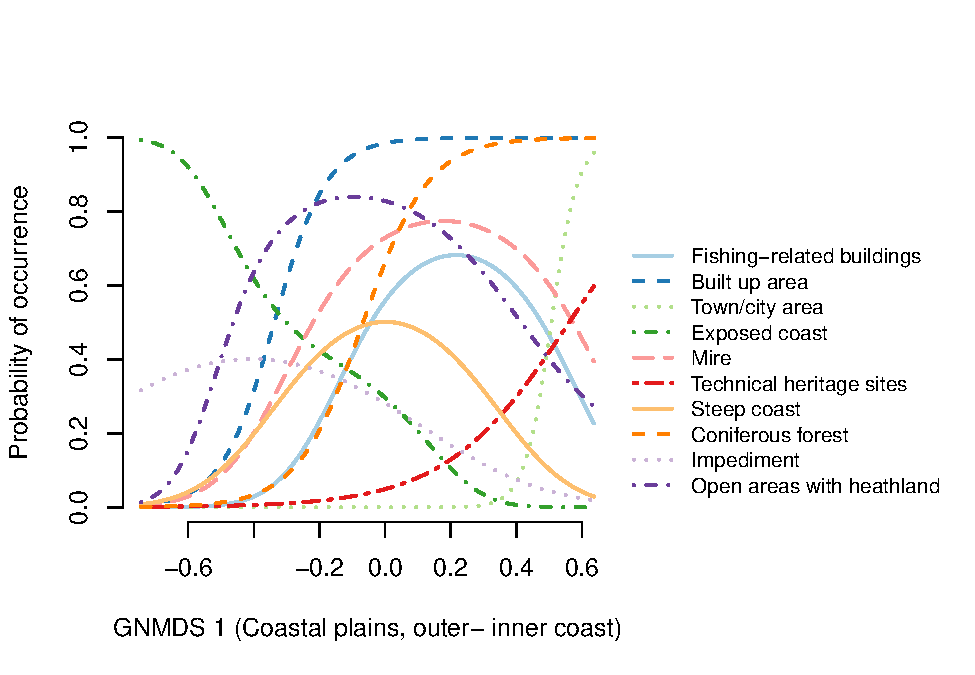
\includegraphics{Landscape_analysis_example_4_files/figure-latex/unnamed-chunk-55-1.pdf}

\begin{Shaded}
\begin{Highlighting}[]
\CommentTok{#2,3,31,44,32, 49,54,68,78,82)}
\end{Highlighting}
\end{Shaded}


\end{document}
